\documentclass[aspectratio=169,10pt]{beamer}

% ===================================================================
% PACKAGES
% ===================================================================
\usepackage[T1]{fontenc}
\usepackage{graphicx}
\usepackage{tikz}
\usepackage{pgfplots}
\usepackage{xcolor}
\usepackage{hyperref}
\usepackage{fontawesome5}
\usepackage{tabularx}
\usepackage{booktabs}
\usepackage{multicol}
\usepackage{calc}
\usepackage{etoolbox}

\usetikzlibrary{shapes.geometric, arrows.meta, positioning, calc, shadows.blur, decorations.markings, backgrounds, fit, patterns}
\pgfplotsset{compat=1.18}

% ===================================================================
% COLOR PALETTE — Modern Corporate + Government Trust
% ===================================================================
\definecolor{primary}{RGB}{10,36,72}        % Deep navy
\definecolor{secondary}{RGB}{0,102,179}     % Bright blue
\definecolor{accent}{RGB}{0,168,120}        % Teal green
\definecolor{accentlight}{RGB}{0,200,150}   % Light teal
\definecolor{warmgold}{RGB}{232,180,52}     % Gold accent
\definecolor{danger}{RGB}{220,53,69}        % Alert red
\definecolor{softgray}{RGB}{240,243,247}    % Background gray
\definecolor{medgray}{RGB}{140,150,165}     % Medium gray
\definecolor{darktext}{RGB}{30,40,55}       % Dark text
\definecolor{cardwhite}{RGB}{255,255,255}   % Card white
\definecolor{gradstart}{RGB}{10,36,72}      % Gradient start
\definecolor{gradend}{RGB}{0,102,179}       % Gradient end
\definecolor{bdgreen}{RGB}{0,106,78}        % Bangladesh green

% ===================================================================
% BEAMER THEME SETUP — Clean Minimal
% ===================================================================
\usetheme{default}
\setbeamertemplate{navigation symbols}{}
\setbeamertemplate{frametitle continuation}{}

% Fonts
\setbeamerfont{title}{size=\LARGE,series=\bfseries}
\setbeamerfont{subtitle}{size=\normalsize}
\setbeamerfont{frametitle}{size=\large,series=\bfseries}
\setbeamerfont{framesubtitle}{size=\small}
\setbeamerfont{footline}{size=\tiny}

% Colors
\setbeamercolor{normal text}{fg=darktext,bg=white}
\setbeamercolor{frametitle}{fg=primary,bg=white}
\setbeamercolor{title}{fg=white}
\setbeamercolor{subtitle}{fg=softgray}
\setbeamercolor{itemize item}{fg=secondary}
\setbeamercolor{itemize subitem}{fg=accent}
\setbeamercolor{block title}{fg=white,bg=secondary}
\setbeamercolor{block body}{fg=darktext,bg=softgray}
\setbeamercolor{alerted text}{fg=danger}

% Itemize style
\setbeamertemplate{itemize item}{\small\raisebox{0.12ex}{\color{secondary}$\blacktriangleright$}}
\setbeamertemplate{itemize subitem}{\scriptsize\raisebox{0.1ex}{\color{accent}\textbullet}}

\hypersetup{colorlinks=true, linkcolor=secondary, urlcolor=secondary}

% ===================================================================
% CUSTOM FRAME TITLE with accent bar
% ===================================================================
\setbeamertemplate{frametitle}{%
  \vspace{0.3cm}%
  \noindent\textcolor{primary}{\insertframetitle}%
  \par\vspace{2pt}%
  \noindent
\begin{tikzpicture}
    \fill[accent] (0,0) rectangle (2.5cm,2pt);
    \fill[secondary!30] (2.5cm,0) rectangle (\textwidth,0.5pt);
  \end{tikzpicture}%
  \vspace{0.15cm}%
}

% ===================================================================
% FOOTER
% ===================================================================
\setbeamertemplate{footline}{%
  \leavevmode%
  \hbox{%
    \begin{beamercolorbox}[wd=0.02\paperwidth,ht=2.5ex,dp=1.2ex]{footline}%
    \end{beamercolorbox}%
    \begin{beamercolorbox}[wd=0.5\paperwidth,ht=2.5ex,dp=1.2ex,left]{footline}%
      \hspace*{0.5em}{\color{medgray}\faIcon{building}~FinkOps UG (Germany) \textbar{} DPE Bangladesh}%
    \end{beamercolorbox}%
    \begin{beamercolorbox}[wd=0.46\paperwidth,ht=2.5ex,dp=1.2ex,right]{footline}%
      {\color{medgray}\insertframenumber{}\,/\,\inserttotalframenumber}\hspace*{1em}%
    \end{beamercolorbox}%
    \begin{beamercolorbox}[wd=0.02\paperwidth,ht=2.5ex,dp=1.2ex]{footline}%
    \end{beamercolorbox}%
  }%
  \vskip0pt%
}

% ===================================================================
% REUSABLE TIKZ COMPONENTS
% ===================================================================
% Stat card
\newcommand{\statcard}[4][secondary]{%
  \begin{tikzpicture}
    \node[rounded corners=6pt, fill=#1!8, draw=#1!25, line width=0.4pt,
          minimum width=3.2cm, minimum height=1.8cm, inner sep=6pt] (box) {%
      \begin{minipage}{2.8cm}\centering
        {\color{#1}\Large #2}\\[3pt]
        {\color{primary}\fontsize{16}{18}\selectfont\bfseries #3}\\[2pt]
        {\color{medgray}\scriptsize #4}
      \end{minipage}
    };
  \end{tikzpicture}%
}

% Icon bullet
\newcommand{\iconbullet}[3][secondary]{{\color{#1}#2}~{#3}}

% Section divider page
\newcommand{\sectionpage}[2]{%
  \begin{frame}[plain]
    \begin{tikzpicture}[remember picture, overlay]
      \fill[primary] (current page.south west) rectangle (current page.north east);
      \fill[secondary, opacity=0.15] ([xshift=-2cm]current page.north east) circle (6cm);
      \fill[accent, opacity=0.08] ([xshift=3cm, yshift=-1cm]current page.south west) circle (5cm);
      \node[anchor=center, text=white] at ([yshift=0.5cm]current page.center) {%
        \begin{minipage}{0.7\textwidth}\centering
          {\fontsize{28}{32}\selectfont\bfseries #1}\\[12pt]
          {\large\color{softgray} #2}
        \end{minipage}
      };
      \draw[accent, line width=2pt] ([xshift=-3cm, yshift=-0.8cm]current page.center) -- ([xshift=3cm, yshift=-0.8cm]current page.center);
    \end{tikzpicture}
  \end{frame}
}

\begin{document}

% ===================================================================
% SLIDE 1 — TITLE PAGE
% ===================================================================
\begin{frame}[plain]
\begin{tikzpicture}[remember picture, overlay]
  % Background gradient
  \fill[left color=gradstart, right color=gradend] (current page.south west) rectangle (current page.north east);
  % Decorative circles
  \fill[white, opacity=0.04] ([xshift=5cm, yshift=2cm]current page.south west) circle (7cm);
  \fill[accent, opacity=0.06] ([xshift=-3cm, yshift=-2cm]current page.north east) circle (5cm);
  \fill[warmgold, opacity=0.05] ([xshift=8cm, yshift=-1cm]current page.north east) circle (3cm);
  % Accent line
  \draw[accent, line width=2.5pt] ([xshift=2cm, yshift=3.2cm]current page.south west) -- ([xshift=7cm, yshift=3.2cm]current page.south west);

  % Logo area
  \node[anchor=north west] at ([xshift=1.5cm, yshift=-1cm]current page.north west) {%
    
\includegraphics[height=1.2cm]{images/government-bangladesh-logo.png}
  };
  % Title content
  \node[anchor=west, text=white] at ([xshift=2cm, yshift=1cm]current page.west) {%
    \begin{minipage}{0.75\textwidth}
      {\fontsize{9}{11}\selectfont\color{accentlight}\textbf{DIRECTORATE OF PRIMARY EDUCATION (DPE) \textbar{} BANGLADESH}}\\[10pt]
      {\fontsize{22}{26}\selectfont\bfseries Transforming Bangladesh's National\\Primary Education Supply System}\\[12pt]
      {\color{softgray}\normalsize Automated Inventory \& Supply Chain Management Platform}\\[6pt]
      {\color{warmgold}\small\faIcon{calendar-alt}~\today}
    \end{minipage}
  };
  % Company badge
  \node[anchor=south east, rounded corners=4pt, fill=white, fill opacity=0.12, text opacity=1] at ([xshift=-1.5cm, yshift=1.5cm]current page.south east) {%
    \begin{minipage}{5cm}\raggedleft
      {\color{white}\small\bfseries FinkOps UG (haftungsbeschr\"ankt)}\\
      {\color{accentlight}\scriptsize German Engineering for National-Scale Impact}
    \end{minipage}
  };
\end{tikzpicture}
\end{frame}

% ===================================================================
% SLIDE 2 — AGENDA
% ===================================================================
\begin{frame}{Presentation Overview}
\begin{columns}[T]
\column{0.55\textwidth}
\vspace{0.3cm}
\begin{tikzpicture}[
  agendaitem/.style={rounded corners=4pt, fill=#1!8, draw=#1!30, line width=0.3pt,
    minimum height=0.7cm, text width=5.5cm, inner sep=5pt, font=\small},
  every node/.style={anchor=west}
]
  \node[agendaitem=secondary] at (0,0)    {\color{secondary}\faIcon{globe-asia}~~\textbf{The Opportunity} — Scale of the Mission};
  \node[agendaitem=danger]    at (0,-1)   {\color{danger}\faIcon{exclamation-triangle}~~\textbf{The Problem} — Current Challenges};
  \node[agendaitem=accent]    at (0,-2)   {\color{accent}\faIcon{lightbulb}~~\textbf{Our Solution} — FinkOps Platform};
  \node[agendaitem=secondary] at (0,-3)   {\color{secondary}\faIcon{shield-alt}~~\textbf{Security} — RBAC + FBAC};
  \node[agendaitem=warmgold]  at (0,-4)   {\color{warmgold}\faIcon{chart-line}~~\textbf{Impact} — Workload \& Outcomes};
  \node[agendaitem=primary]   at (0,-5)   {\color{primary}\faIcon{server}~~\textbf{Architecture \& Technology}};
  \node[agendaitem=accent]    at (0,-6)   {\color{accent}\faIcon{road}~~\textbf{Roadmap \& Next Steps}};
\end{tikzpicture}

\column{0.42\textwidth}
\vspace{0.2cm}
\begin{tikzpicture}
  \node[rounded corners=8pt, draw=softgray, line width=0.5pt, inner sep=0pt, drop shadow={shadow xshift=1pt, shadow yshift=-1pt, opacity=0.1}] {%
    
\includegraphics[width=\textwidth]{images/DPE_cover.png}
  };
\end{tikzpicture}
\end{columns}
\end{frame}

% ===================================================================
% SECTION: THE OPPORTUNITY
% ===================================================================
\sectionpage{The Opportunity}{One of the World's Largest Education Ecosystems}

% ===================================================================
% SLIDE 3 — NATIONAL SCALE
% ===================================================================
\begin{frame}{A National System of Unprecedented Scale}
\vspace{0.1cm}
\begin{center}
\statcard[secondary]{\faIcon{school}}{66,000+}{Primary Schools}
\hspace{0.3cm}
\statcard[accent]{\faIcon{user-graduate}}{20.5M}{Students}
\hspace{0.3cm}
\statcard[warmgold]{\faIcon{users}}{500,000+}{Staff Members}
\hspace{0.3cm}
\statcard[primary]{\faIcon{sitemap}}{8 / 64 / 514}{Div / Dist / Upazila}
\end{center}

\vspace{0.3cm}
\begin{columns}[T]
\column{0.48\textwidth}
\textbf{\color{primary}Administrative Network:}
\begin{itemize}
  \item 8 Divisions with main warehouses
  \item 64 District Primary Education Offices
  \item 514 Upazila Education Offices
  \item 505 Upazila Resource Centers (URCs)
  \item 67 Primary Teachers Training Institutes
\end{itemize}

\column{0.48\textwidth}
\textbf{\color{primary}Supply Categories Managed:}
\begin{itemize}
  \item Stationery \& teaching materials
  \item ICT equipment (PCs, SSDs, RAM, peripherals)
  \item Printer consumables (HP/Brother/Samsung)
  \item Furniture \& maintenance items
  \item Photocopier supplies \& training materials
\end{itemize}
\end{columns}

\vspace{0.2cm}
\begin{center}

\begin{tikzpicture}
  \node[rounded corners=4pt, fill=accent!10, inner sep=6pt] {%
    {\color{accent}\faIcon{check-circle}~\textbf{One of the world's largest education ecosystems — requiring industrial-grade logistics.}}
  };
\end{tikzpicture}
\end{center}
\end{frame}

% ===================================================================
% SECTION: THE PROBLEM
% ===================================================================
\sectionpage{The Problem}{Why the Current System Cannot Scale}

% ===================================================================
% SLIDE 4 — CHALLENGES
% ===================================================================
\begin{frame}{System Challenges Today}
\begin{columns}[T]
\column{0.48\textwidth}
\begin{tikzpicture}
  \node[rounded corners=6pt, fill=danger!6, draw=danger!20, line width=0.3pt,
        inner sep=8pt, text width=6cm] {%
    \textbf{\color{danger}\faIcon{times-circle}~Operational Pain Points}\\[6pt]
    \begin{minipage}{5.5cm}\small
    \iconbullet[danger]{\faIcon{file-alt}}{Manual, paper-based workflows}\\[3pt]
    \iconbullet[danger]{\faIcon{clock}}{Slow requisition \& approval cycles}\\[3pt]
    \iconbullet[danger]{\faIcon{eye-slash}}{No real-time visibility across tiers}\\[3pt]
    \iconbullet[danger]{\faIcon{keyboard}}{High data entry error rates}\\[3pt]
    \iconbullet[danger]{\faIcon{search}}{Difficult \& time-consuming audits}\\[3pt]
    \iconbullet[danger]{\faIcon{chart-bar}}{Zero forecasting capability}
    \end{minipage}
  };
\end{tikzpicture}

\column{0.48\textwidth}
\begin{tikzpicture}
  \node[rounded corners=6pt, fill=primary!5, draw=primary!15, line width=0.3pt,
        inner sep=8pt, text width=6cm] {%
    \textbf{\color{primary}\faIcon{exclamation-triangle}~Impact on DPE}\\[6pt]
    \begin{minipage}{5.5cm}\small
    \iconbullet[primary]{\faIcon{money-bill-wave}}{Resource misuse \& financial loss}\\[3pt]
    \iconbullet[primary]{\faIcon{boxes}}{Overstocking / critical stockouts}\\[3pt]
    \iconbullet[primary]{\faIcon{user-shield}}{Lack of accountability}\\[3pt]
    \iconbullet[primary]{\faIcon{briefcase}}{Excessive officer workload}\\[3pt]
    \iconbullet[primary]{\faIcon{hourglass-half}}{Delayed reporting to HQ}\\[3pt]
    \iconbullet[primary]{\faIcon{balance-scale}}{Governance \& compliance risk}
    \end{minipage}
  };
\end{tikzpicture}
\end{columns}

\vspace{0.4cm}
\begin{center}

\begin{tikzpicture}
  \node[rounded corners=4pt, fill=danger!8, inner sep=6pt] {%
    {\color{danger}\faIcon{arrow-right}~\textbf{Manual complexity leads to loss, delays, misuse, and heavy officer workload across 66,000+ nodes.}}
  };
\end{tikzpicture}
\end{center}
\end{frame}

% ===================================================================
% SECTION: OUR SOLUTION
% ===================================================================
\sectionpage{Our Solution}{FinkOps — A Single National Digital Platform}

% ===================================================================
% SLIDE 5 — PLATFORM OVERVIEW
% ===================================================================
\begin{frame}{FinkOps: One Platform for the Entire Nation}
\begin{center}
\begin{tikzpicture}
  \node[rounded corners=8pt, draw=softgray, line width=0.5pt, inner sep=0pt,
        drop shadow={shadow xshift=1pt, shadow yshift=-1pt, opacity=0.08}] {%
    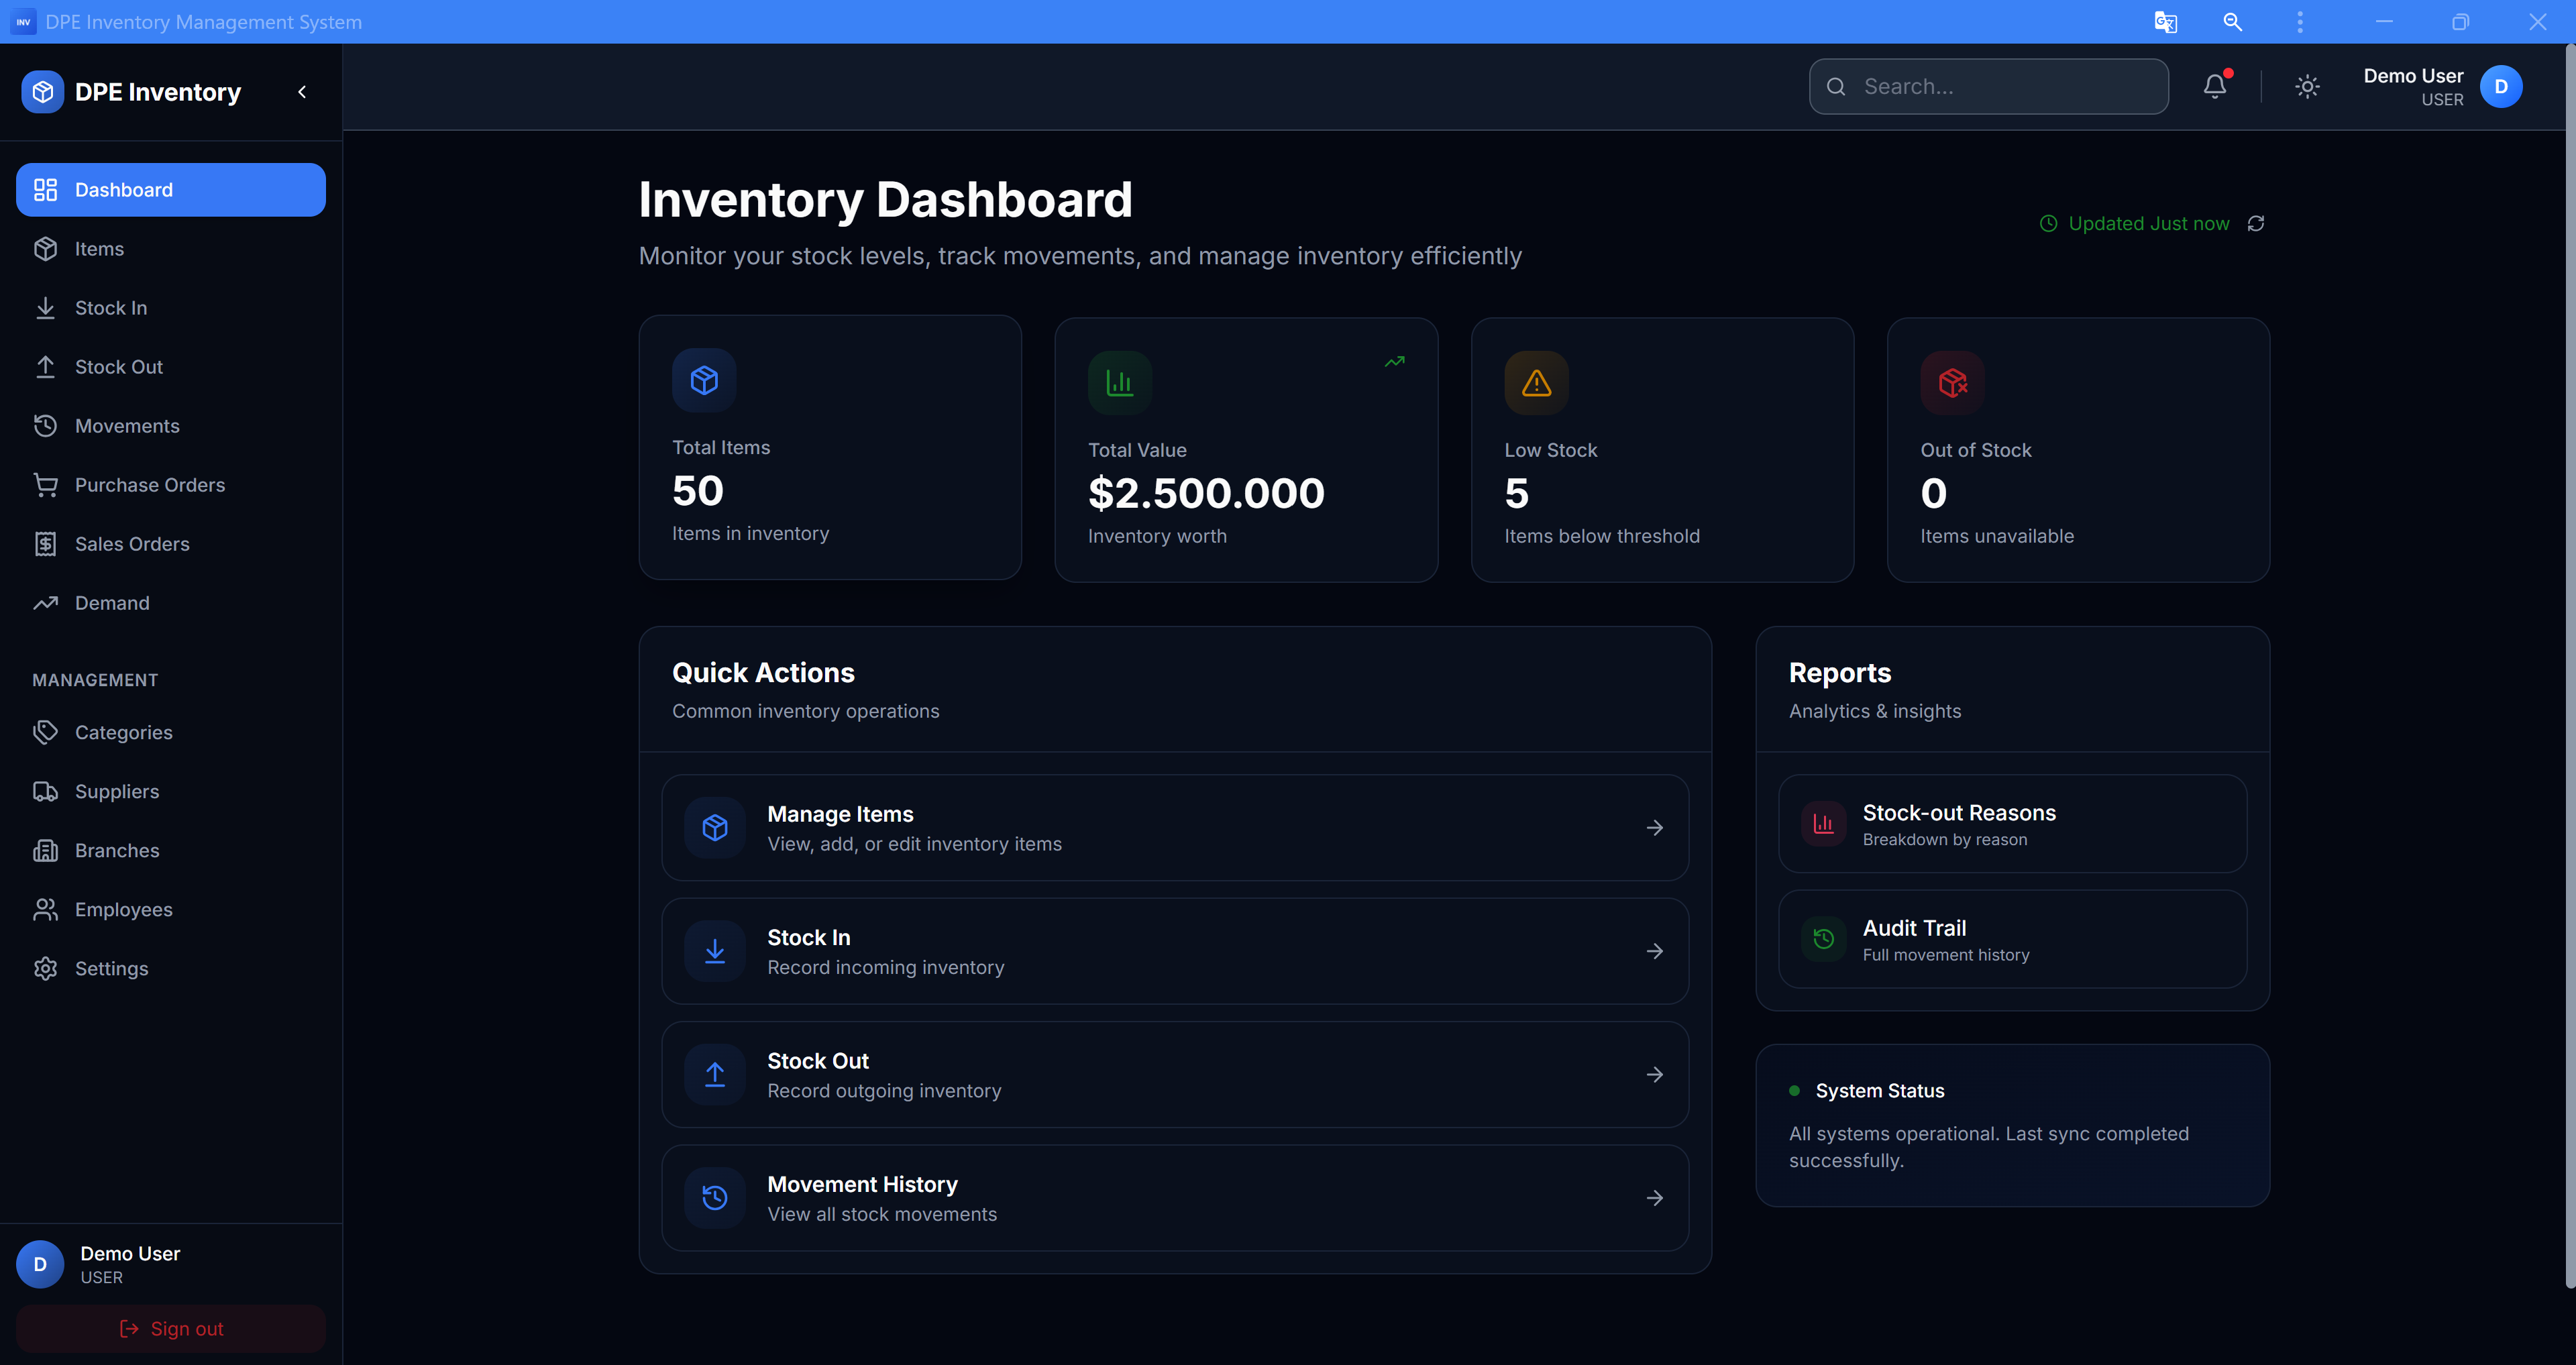
\includegraphics[width=0.82\textwidth, height=3.5cm, keepaspectratio]{images/dashboard-home.png}
  };
\end{tikzpicture}
\end{center}

\vspace{0.15cm}
\begin{columns}[T]
\column{0.48\textwidth}
\begin{itemize}\small
  \item[\color{accent}\faIcon{check}] Real-time visibility from HQ to School
  \item[\color{accent}\faIcon{check}] Automated procurement with forecasting
  \item[\color{accent}\faIcon{check}] RBAC + FBAC (Feature-Based Access Control)
\end{itemize}

\column{0.48\textwidth}
\begin{itemize}\small
  \item[\color{accent}\faIcon{check}] Fully digital \& immutable audit trails
  \item[\color{accent}\faIcon{check}] Offline-first PWA for field operations
  \item[\color{accent}\faIcon{check}] \textbf{80--90\% reduction in officer workload}
\end{itemize}
\end{columns}
\end{frame}

% ===================================================================
% SLIDE 6 — CORE MODULES (6-card grid)
% ===================================================================
\begin{frame}{Core System Modules}
\vspace{0.1cm}
\begin{center}
\begin{tikzpicture}[
  modcard/.style={rounded corners=6pt, fill=#1!7, draw=#1!25, line width=0.3pt,
    minimum width=4.6cm, minimum height=1.6cm, inner sep=5pt}
]
  % Row 1
  \node[modcard=secondary] (m1) at (0,0) {%
    \begin{minipage}{4.2cm}
      {\color{secondary}\faIcon{chart-line}~\textbf{\small Demand \& Planning}}\\
      {\scriptsize Forecasts per school using historical data \& academic calendars}
    \end{minipage}};
  \node[modcard=accent] (m2) at (5.2,0) {%
    \begin{minipage}{4.2cm}
      {\color{accent}\faIcon{shopping-cart}~\textbf{\small Procurement}}\\
      {\scriptsize Auto-PO suggestions, tender alignment, budget guardrails}
    \end{minipage}};
  \node[modcard=warmgold] (m3) at (10.4,0) {%
    \begin{minipage}{4.2cm}
      {\color{warmgold}\faIcon{warehouse}~\textbf{\small Warehouse \& Inventory}}\\
      {\scriptsize GRN, stock levels, expiry monitoring, cycle counts}
    \end{minipage}};
  % Row 2
  \node[modcard=primary] (m4) at (0,-2.2) {%
    \begin{minipage}{4.2cm}
      {\color{primary}\faIcon{truck}~\textbf{\small Distribution}}\\
      {\scriptsize Allocation, routing, proof of delivery via QR/OTP}
    \end{minipage}};
  \node[modcard=danger] (m5) at (5.2,-2.2) {%
    \begin{minipage}{4.2cm}
      {\color{danger}\faIcon{tags}~\textbf{\small Asset Management}}\\
      {\scriptsize Asset tags, warranty tracking, consumable cycles}
    \end{minipage}};
  \node[modcard=secondary] (m6) at (10.4,-2.2) {%
    \begin{minipage}{4.2cm}
      {\color{secondary}\faIcon{chart-pie}~\textbf{\small Insights \& Compliance}}\\
      {\scriptsize Dashboards, audit exports, exception alerts}
    \end{minipage}};
\end{tikzpicture}
\end{center}

\vspace{0.2cm}
\begin{center}

\begin{tikzpicture}
  \node[rounded corners=4pt, fill=secondary!8, inner sep=5pt] {%
    {\color{secondary}\small\faIcon{puzzle-piece}~All modules work together as a unified national platform — not isolated tools.}
  };
\end{tikzpicture}
\end{center}
\end{frame}

% ===================================================================
% SLIDE 7 — FBAC (Feature-Based Access Control)
% ===================================================================
\begin{frame}{Feature-Based Access Control (FBAC)}
\begin{columns}[T]
\column{0.45\textwidth}
\vspace{0.2cm}
\textbf{\color{primary}Why FBAC Matters for DPE:}
\begin{itemize}\small
  \item Prevents unauthorized modifications at feature level
  \item Enforces zero-trust across 66,000+ schools
  \item Essential for multi-tier approval workflows
  \item Stronger governance \& audit readiness
  \item Goes beyond RBAC — controls every button, action, data field
\end{itemize}

\vspace{0.3cm}

\begin{tikzpicture}
  \node[rounded corners=4pt, fill=accent!8, inner sep=5pt, text width=5.5cm] {%
    {\color{accent}\scriptsize\faIcon{shield-alt}~\textbf{FBAC is our competitive advantage} — most vendors only offer basic RBAC. FinkOps provides feature-granular security.}
  };
\end{tikzpicture}

\column{0.52\textwidth}
\vspace{0.1cm}
\begin{center}
\begin{tikzpicture}[
  node distance=1cm,
  flowbox/.style={rounded corners=5pt, minimum width=4.5cm, minimum height=0.65cm,
    font=\small\bfseries, text=white, drop shadow={shadow xshift=0.5pt, shadow yshift=-0.5pt, opacity=0.15}},
  arr/.style={-{Stealth[length=5pt]}, thick, color=medgray}
]
  \node[flowbox, fill=secondary] (login) {\faIcon{sign-in-alt}~User Login};
  \node[flowbox, fill=accent, below=of login] (auth) {\faIcon{fingerprint}~Identity \& 2FA};
  \node[flowbox, fill=primary, below=of auth] (fbac) {\faIcon{shield-alt}~FBAC Permission Engine};
  \node[flowbox, fill=warmgold, text=primary, below=of fbac] (ui) {\faIcon{desktop}~Application UI};

  \draw[arr] (login) -- (auth);
  \draw[arr] (auth) -- (fbac);
  \draw[arr] (fbac) -- (ui);

  % Side annotations
  \node[right=0.4cm of fbac, font=\scriptsize, text=medgray, text width=2.8cm] {%
    Checks:\\
    \textbullet~Feature access?\\
    \textbullet~Action permitted?\\
    \textbullet~Data scope?
  };
\end{tikzpicture}
\end{center}
\end{columns}
\end{frame}

% ===================================================================
% SLIDE 8 — FBAC PERMISSION MATRIX
% ===================================================================
\begin{frame}{FBAC Permission Matrix}
\vspace{0.1cm}
\begin{center}
\small
\renewcommand{\arraystretch}{1.3}
\begin{tabularx}{0.95\textwidth}{l *{6}{>{\centering\arraybackslash}X}}
\toprule
\textbf{\color{primary}Feature} & \textbf{School} & \textbf{URC} & \textbf{Upazila} & \textbf{District} & \textbf{HQ/DPE} & \textbf{Auditor} \\
\midrule
Create Requisition    & \color{accent}\faIcon{check} & \color{accent}\faIcon{check} & \color{accent}\faIcon{check} & \color{medgray}\faIcon{times} & \color{medgray}\faIcon{times} & \color{medgray}\faIcon{times} \\
Approve Requisition   & \color{medgray}\faIcon{times} & \color{medgray}\faIcon{times} & \color{accent}\faIcon{check} & \color{accent}\faIcon{check} & \color{accent}\faIcon{check} & \color{medgray}\faIcon{times} \\
View Stock            & \color{accent}\faIcon{check} & \color{accent}\faIcon{check} & \color{accent}\faIcon{check} & \color{accent}\faIcon{check} & \color{accent}\faIcon{check} & \color{accent}\faIcon{check} \\
Modify Stock          & \color{medgray}\faIcon{times} & \color{medgray}\faIcon{times} & \color{accent}\faIcon{check} & \color{accent}\faIcon{check} & \color{accent}\faIcon{check} & \color{medgray}\faIcon{times} \\
Create Procurement PO & \color{medgray}\faIcon{times} & \color{medgray}\faIcon{times} & \color{medgray}\faIcon{times} & \color{medgray}\faIcon{times} & \color{accent}\faIcon{check} & \color{medgray}\faIcon{times} \\
View Audit Logs       & \color{medgray}\faIcon{times} & \color{medgray}\faIcon{times} & \color{medgray}\faIcon{times} & \color{medgray}\faIcon{times} & \color{accent}\faIcon{check} & \color{accent}\faIcon{check} \\
Export Reports        & \color{accent}\faIcon{check} & \color{accent}\faIcon{check} & \color{accent}\faIcon{check} & \color{accent}\faIcon{check} & \color{accent}\faIcon{check} & \color{accent}\faIcon{check} \\
Override Distribution & \color{medgray}\faIcon{times} & \color{medgray}\faIcon{times} & \color{medgray}\faIcon{times} & \color{accent}\faIcon{check} & \color{accent}\faIcon{check} & \color{medgray}\faIcon{times} \\
\bottomrule
\end{tabularx}
\end{center}

\vspace{0.2cm}
\begin{center}

\begin{tikzpicture}
  \node[rounded corners=4pt, fill=primary!6, inner sep=5pt] {%
    {\color{primary}\small\faIcon{lock}~Every action, screen, and data field is protected — preventing unauthorized changes across all tiers.}
  };
\end{tikzpicture}
\end{center}
\end{frame}

% ===================================================================
% SECTION: IMPACT
% ===================================================================
\sectionpage{Impact \& Outcomes}{Measurable Results for DPE}

% ===================================================================
% SLIDE 9 — WORKLOAD REDUCTION
% ===================================================================
\begin{frame}{80--90\% Officer Workload Reduction}
\begin{columns}[T]
\column{0.45\textwidth}
\vspace{0.1cm}
\textbf{\color{primary}How Workload Drops:}
\begin{itemize}\small
  \item[\color{accent}\faIcon{robot}] No manual data entry — one input updates all
  \item[\color{accent}\faIcon{file-export}] No compiling stock reports from schools
  \item[\color{accent}\faIcon{mouse-pointer}] One-click requisition approvals
  \item[\color{accent}\faIcon{magic}] Automated purchase suggestions
  \item[\color{accent}\faIcon{tachometer-alt}] Instant district/division reporting
  \item[\color{accent}\faIcon{receipt}] Digital receipts replace physical files
\end{itemize}

\vspace{0.2cm}

\begin{tikzpicture}
  \node[rounded corners=4pt, fill=accent!8, inner sep=5pt, text width=5.5cm] {%
    {\color{accent}\scriptsize\faIcon{quote-left}~Officers get time back for real education tasks — monitoring, mentoring, and quality improvement.}
  };
\end{tikzpicture}

\column{0.52\textwidth}
\vspace{0.1cm}
\begin{center}
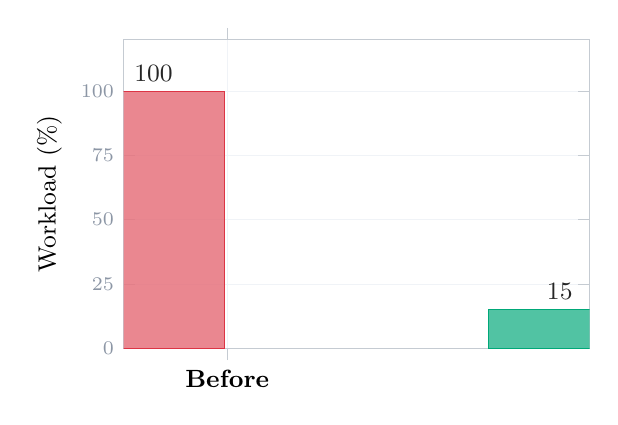
\begin{tikzpicture}
\begin{axis}[
    ybar,
    ymin=0, ymax=120,
    width=7.5cm, height=5.5cm,
    symbolic x coords={Before, After FinkOps},
    xtick=data,
    ylabel={\small Workload (\%)},
    ylabel style={font=\small},
    bar width=1.8cm,
    nodes near coords,
    nodes near coords style={font=\small\bfseries},
    every axis plot/.append style={fill opacity=0.85},
    axis line style={draw=medgray!50},
    tick style={draw=medgray!50},
    ytick={0,25,50,75,100},
    yticklabel style={font=\scriptsize, color=medgray},
    xticklabel style={font=\small\bfseries},
    enlarge x limits=0.4,
    grid=major,
    grid style={draw=softgray, line width=0.3pt},
]
\addplot[fill=danger!70, draw=danger] coordinates {(Before,100)};
\addplot[fill=accent!80, draw=accent] coordinates {(After FinkOps,15)};
\end{axis}
\end{tikzpicture}

\vspace{0.1cm}
{\color{accent}\small\textbf{85\% reduction} — from 100\% manual to 15\% oversight only}
\end{center}
\end{columns}
\end{frame}

% ===================================================================
% SLIDE 10 — EXPECTED OUTCOMES
% ===================================================================
\begin{frame}{Expected Outcomes}
\begin{columns}[T]
\column{0.48\textwidth}
\begin{tikzpicture}
  \node[rounded corners=6pt, fill=accent!6, draw=accent!20, line width=0.3pt,
        inner sep=8pt, text width=6cm] {%
    \textbf{\color{accent}\faIcon{cogs}~Operational Improvements}\\[6pt]
    \begin{minipage}{5.5cm}\small
    \iconbullet[accent]{\faIcon{check-circle}}{Eliminate manual errors entirely}\\[3pt]
    \iconbullet[accent]{\faIcon{bolt}}{Reduce processing time by 85\%+}\\[3pt]
    \iconbullet[accent]{\faIcon{eye}}{Real-time visibility across all levels}\\[3pt]
    \iconbullet[accent]{\faIcon{sync-alt}}{Automated requisition workflows}\\[3pt]
    \iconbullet[accent]{\faIcon{file-download}}{Instant reporting capabilities}
    \end{minipage}
  };
\end{tikzpicture}

\column{0.48\textwidth}
\begin{tikzpicture}
  \node[rounded corners=6pt, fill=secondary!6, draw=secondary!20, line width=0.3pt,
        inner sep=8pt, text width=6cm] {%
    \textbf{\color{secondary}\faIcon{balance-scale}~Financial \& Governance}\\[6pt]
    \begin{minipage}{5.5cm}\small
    \iconbullet[secondary]{\faIcon{hand-holding-usd}}{Prevent resource misuse}\\[3pt]
    \iconbullet[secondary]{\faIcon{chart-line}}{Reduce financial losses}\\[3pt]
    \iconbullet[secondary]{\faIcon{tasks}}{Judicious resource utilization}\\[3pt]
    \iconbullet[secondary]{\faIcon{university}}{Institutional accountability}\\[3pt]
    \iconbullet[secondary]{\faIcon{star}}{Improved service delivery quality}
    \end{minipage}
  };
\end{tikzpicture}
\end{columns}

\vspace{0.4cm}
\begin{center}

\begin{tikzpicture}
  \node[rounded corners=5pt, fill=accent!10, inner sep=8pt] {%
    {\color{accent}\large\faIcon{award}~\textbf{Good governance through automation, transparency, and accountability.}}
  };
\end{tikzpicture}
\end{center}
\end{frame}

% ===================================================================
% SECTION: ARCHITECTURE
% ===================================================================
\sectionpage{Architecture}{National Hierarchical System Design}

% ===================================================================
% SLIDE 11 — HIERARCHICAL ARCHITECTURE
% ===================================================================
\begin{frame}{National Hierarchical Architecture}
\begin{center}
\begin{tikzpicture}[
  level/.style={rounded corners=5pt, minimum height=0.6cm, font=\small\bfseries, text=white,
    drop shadow={shadow xshift=0.5pt, shadow yshift=-0.5pt, opacity=0.1}},
  arr/.style={-{Stealth[length=4pt]}, thick, color=medgray!70},
  scale=0.95
]
  % HQ
  \node[level, fill=primary, minimum width=5cm] (hq) at (0,5.5) {\faIcon{building}~DPE Headquarters};

  % Divisions
  \node[level, fill=secondary, minimum width=3.5cm] (div1) at (-4,4) {\faIcon{city}~Division 1};
  \node[level, fill=secondary, minimum width=3.5cm] (div2) at (4,4) {\faIcon{city}~Division 2};

  % Districts
  \node[level, fill=secondary!70, minimum width=2.5cm, font=\scriptsize\bfseries] (dist1) at (-5.5,2.5) {District A};
  \node[level, fill=secondary!70, minimum width=2.5cm, font=\scriptsize\bfseries] (dist2) at (-2.5,2.5) {District B};
  \node[level, fill=secondary!70, minimum width=2.5cm, font=\scriptsize\bfseries] (dist3) at (2.5,2.5) {District C};
  \node[level, fill=secondary!70, minimum width=2.5cm, font=\scriptsize\bfseries] (dist4) at (5.5,2.5) {District D};

  % Upazilas
  \node[level, fill=accent, minimum width=2cm, font=\scriptsize\bfseries] (upz1) at (-5.5,1) {Upazila};
  \node[level, fill=accent, minimum width=2cm, font=\scriptsize\bfseries] (upz2) at (-2.5,1) {Upazila};
  \node[level, fill=accent, minimum width=2cm, font=\scriptsize\bfseries] (upz3) at (2.5,1) {Upazila};
  \node[level, fill=accent, minimum width=2cm, font=\scriptsize\bfseries] (upz4) at (5.5,1) {Upazila};

  % Schools
  \node[level, fill=warmgold, text=primary, minimum width=1.8cm, font=\scriptsize\bfseries] (s1) at (-5.5,-0.4) {\faIcon{school}~School};
  \node[level, fill=warmgold, text=primary, minimum width=1.8cm, font=\scriptsize\bfseries] (s2) at (-2.5,-0.4) {\faIcon{school}~School};
  \node[level, fill=warmgold, text=primary, minimum width=1.8cm, font=\scriptsize\bfseries] (s3) at (2.5,-0.4) {\faIcon{school}~School};
  \node[level, fill=warmgold, text=primary, minimum width=1.8cm, font=\scriptsize\bfseries] (s4) at (5.5,-0.4) {\faIcon{school}~School};

  % Arrows
  \draw[arr] (hq) -- (div1);
  \draw[arr] (hq) -- (div2);
  \draw[arr] (div1) -- (dist1);
  \draw[arr] (div1) -- (dist2);
  \draw[arr] (div2) -- (dist3);
  \draw[arr] (div2) -- (dist4);
  \draw[arr] (dist1) -- (upz1);
  \draw[arr] (dist2) -- (upz2);
  \draw[arr] (dist3) -- (upz3);
  \draw[arr] (dist4) -- (upz4);
  \draw[arr] (upz1) -- (s1);
  \draw[arr] (upz2) -- (s2);
  \draw[arr] (upz3) -- (s3);
  \draw[arr] (upz4) -- (s4);

  % Flow labels
  \node[font=\scriptsize, text=secondary, rotate=90] at (-7.5,2.5) {\faIcon{arrow-down}~Supply Flow};
  \node[font=\scriptsize, text=accent, rotate=90] at (7.5,2.5) {\faIcon{arrow-up}~Demand Flow};
\end{tikzpicture}
\end{center}

\vspace{0.1cm}
\begin{center}
{\small\color{secondary}\textbf{Supply:} HQ $\rightarrow$ Division $\rightarrow$ District $\rightarrow$ Upazila $\rightarrow$ School \hspace{1cm}
\color{accent}\textbf{Demand:} School $\rightarrow$ Upazila $\rightarrow$ District $\rightarrow$ Division $\rightarrow$ HQ}
\end{center}
\end{frame}

% ===================================================================
% SLIDE 12 — TECHNOLOGY STACK
% ===================================================================
\begin{frame}{Technology Stack}
\begin{columns}[T]
\column{0.32\textwidth}
\begin{tikzpicture}
  \node[rounded corners=6pt, fill=secondary!6, draw=secondary!20, line width=0.3pt,
        inner sep=7pt, text width=4.2cm, minimum height=4.5cm] {%
    \textbf{\color{secondary}\faIcon{desktop}~Frontend}\\[6pt]
    \begin{minipage}{3.8cm}\scriptsize
    \iconbullet[secondary]{\faIcon{react}}{Next.js 16+ (React)}\\[2pt]
    \iconbullet[secondary]{\faIcon{code}}{TypeScript}\\[2pt]
    \iconbullet[secondary]{\faIcon{paint-brush}}{Tailwind CSS}\\[2pt]
    \iconbullet[secondary]{\faIcon{mobile-alt}}{PWA + Mobile Apps}\\[2pt]
    \iconbullet[secondary]{\faIcon{laptop}}{Desktop Support}\\[2pt]
    \iconbullet[secondary]{\faIcon{wifi}}{Offline-First Design}
    \end{minipage}
  };
\end{tikzpicture}

\column{0.32\textwidth}
\begin{tikzpicture}
  \node[rounded corners=6pt, fill=accent!6, draw=accent!20, line width=0.3pt,
        inner sep=7pt, text width=4.2cm, minimum height=4.5cm] {%
    \textbf{\color{accent}\faIcon{server}~Backend}\\[6pt]
    \begin{minipage}{3.8cm}\scriptsize
    \iconbullet[accent]{\faIcon{java}}{Spring Boot (Java)}\\[2pt]
    \iconbullet[accent]{\faIcon{plug}}{RESTful API}\\[2pt]
    \iconbullet[accent]{\faIcon{database}}{PostgreSQL}\\[2pt]
    \iconbullet[accent]{\faIcon{key}}{JWT + 2FA Auth}\\[2pt]
    \iconbullet[accent]{\faIcon{cubes}}{Microservices Ready}\\[2pt]
    \iconbullet[accent]{\faIcon{cloud}}{Cloud-Native Deploy}
    \end{minipage}
  };
\end{tikzpicture}

\column{0.32\textwidth}

\begin{tikzpicture}
  \node[rounded corners=6pt, fill=primary!6, draw=primary!15, line width=0.3pt,
        inner sep=7pt, text width=4.2cm, minimum height=4.5cm] {%
    \textbf{\color{primary}\faIcon{shield-alt}~Security}\\[6pt]
    \begin{minipage}{3.8cm}\scriptsize
    \iconbullet[primary]{\faIcon{lock}}{End-to-end Encryption}\\[2pt]
    \iconbullet[primary]{\faIcon{certificate}}{ISO27001 Aligned}\\[2pt]
    \iconbullet[primary]{\faIcon{user-lock}}{RBAC + FBAC}\\[2pt]
    \iconbullet[primary]{\faIcon{history}}{Immutable Audit Logs}\\[2pt]
    \iconbullet[primary]{\faIcon{globe-europe}}{GDPR Compliant}\\[2pt]
    \iconbullet[primary]{\faIcon{hdd}}{Data Residency Options}
    \end{minipage}
  };
\end{tikzpicture}
\end{columns}
\end{frame}

% ===================================================================
% SECTION: LIVE DEMO
% ===================================================================
\sectionpage{Live Demo}{See the Platform in Action}

% ===================================================================
% SLIDE 13 — DEMO SCREENSHOTS GRID
% ===================================================================
\begin{frame}{Platform Screenshots}
\begin{center}
\begin{tikzpicture}[
  imgframe/.style={rounded corners=4pt, draw=softgray, line width=0.4pt, inner sep=0pt,
    drop shadow={shadow xshift=0.5pt, shadow yshift=-0.5pt, opacity=0.06}}
]
  % Row 1
  \node[imgframe] at (0,0) {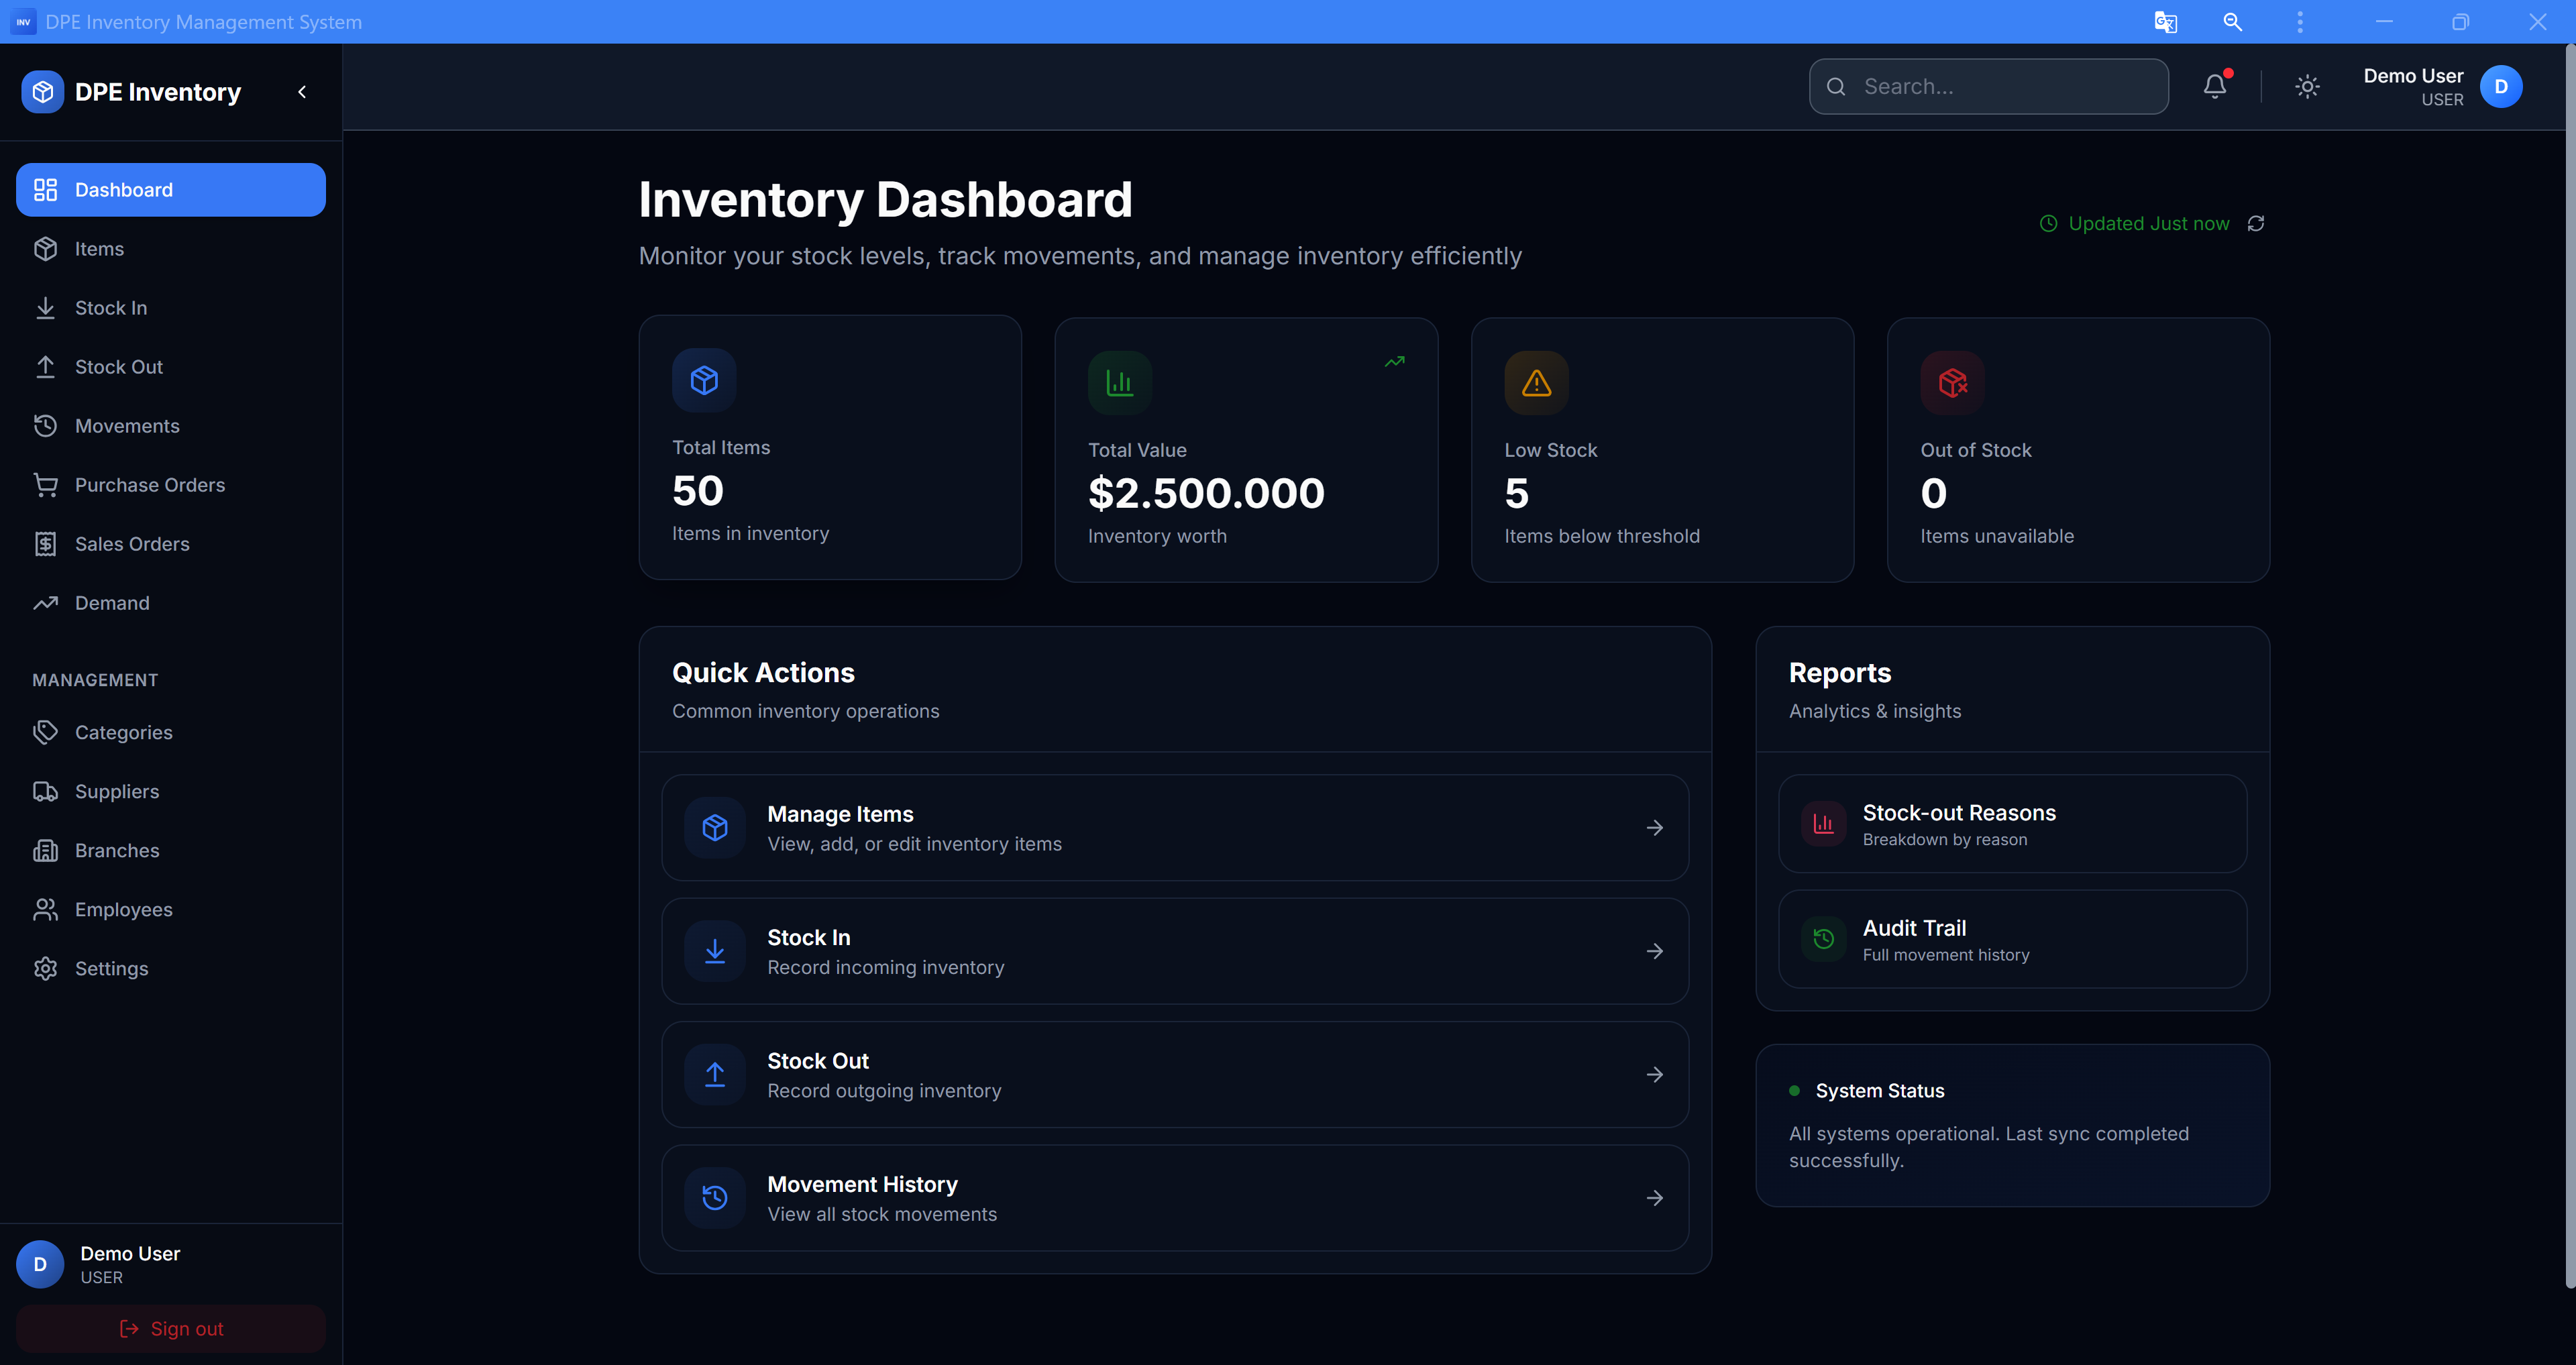
\includegraphics[width=3.6cm, height=2cm]{images/dashboard-home.png}};
  \node[font=\tiny\bfseries, color=secondary] at (0,-1.2) {Dashboard Home};

  \node[imgframe] at (4.2,0) {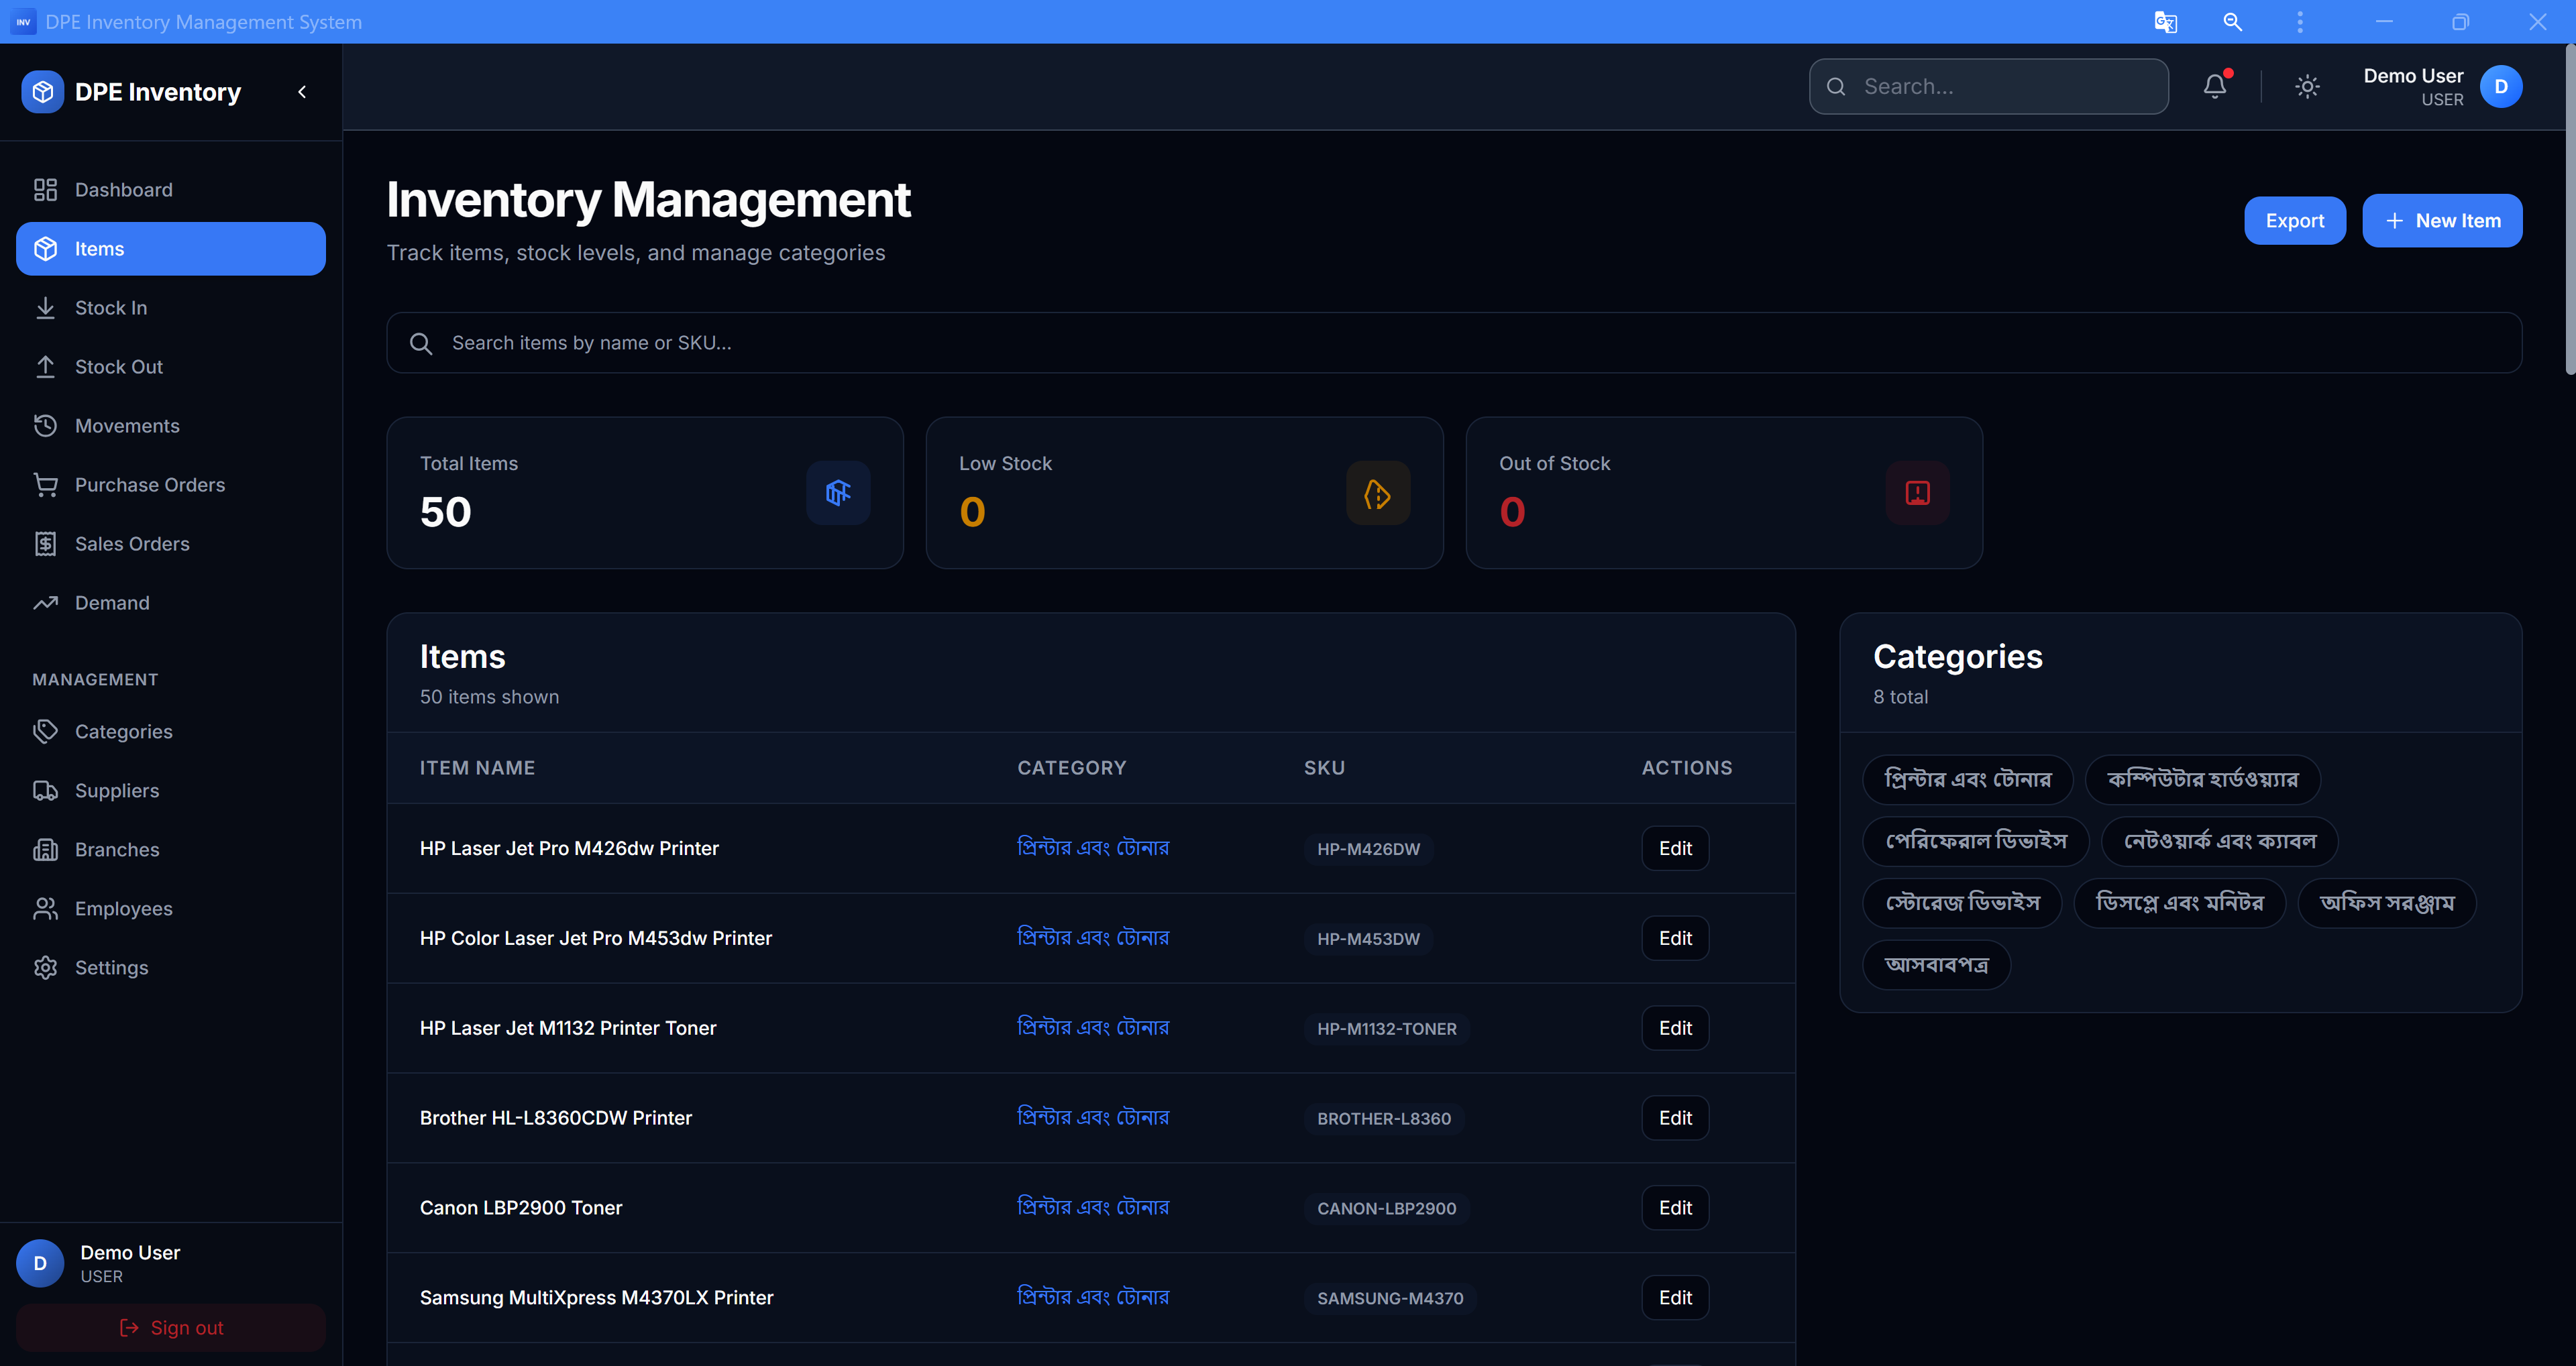
\includegraphics[width=3.6cm, height=2cm]{images/item-dashboard.png}};
  \node[font=\tiny\bfseries, color=secondary] at (4.2,-1.2) {Item Management};

  \node[imgframe] at (8.4,0) {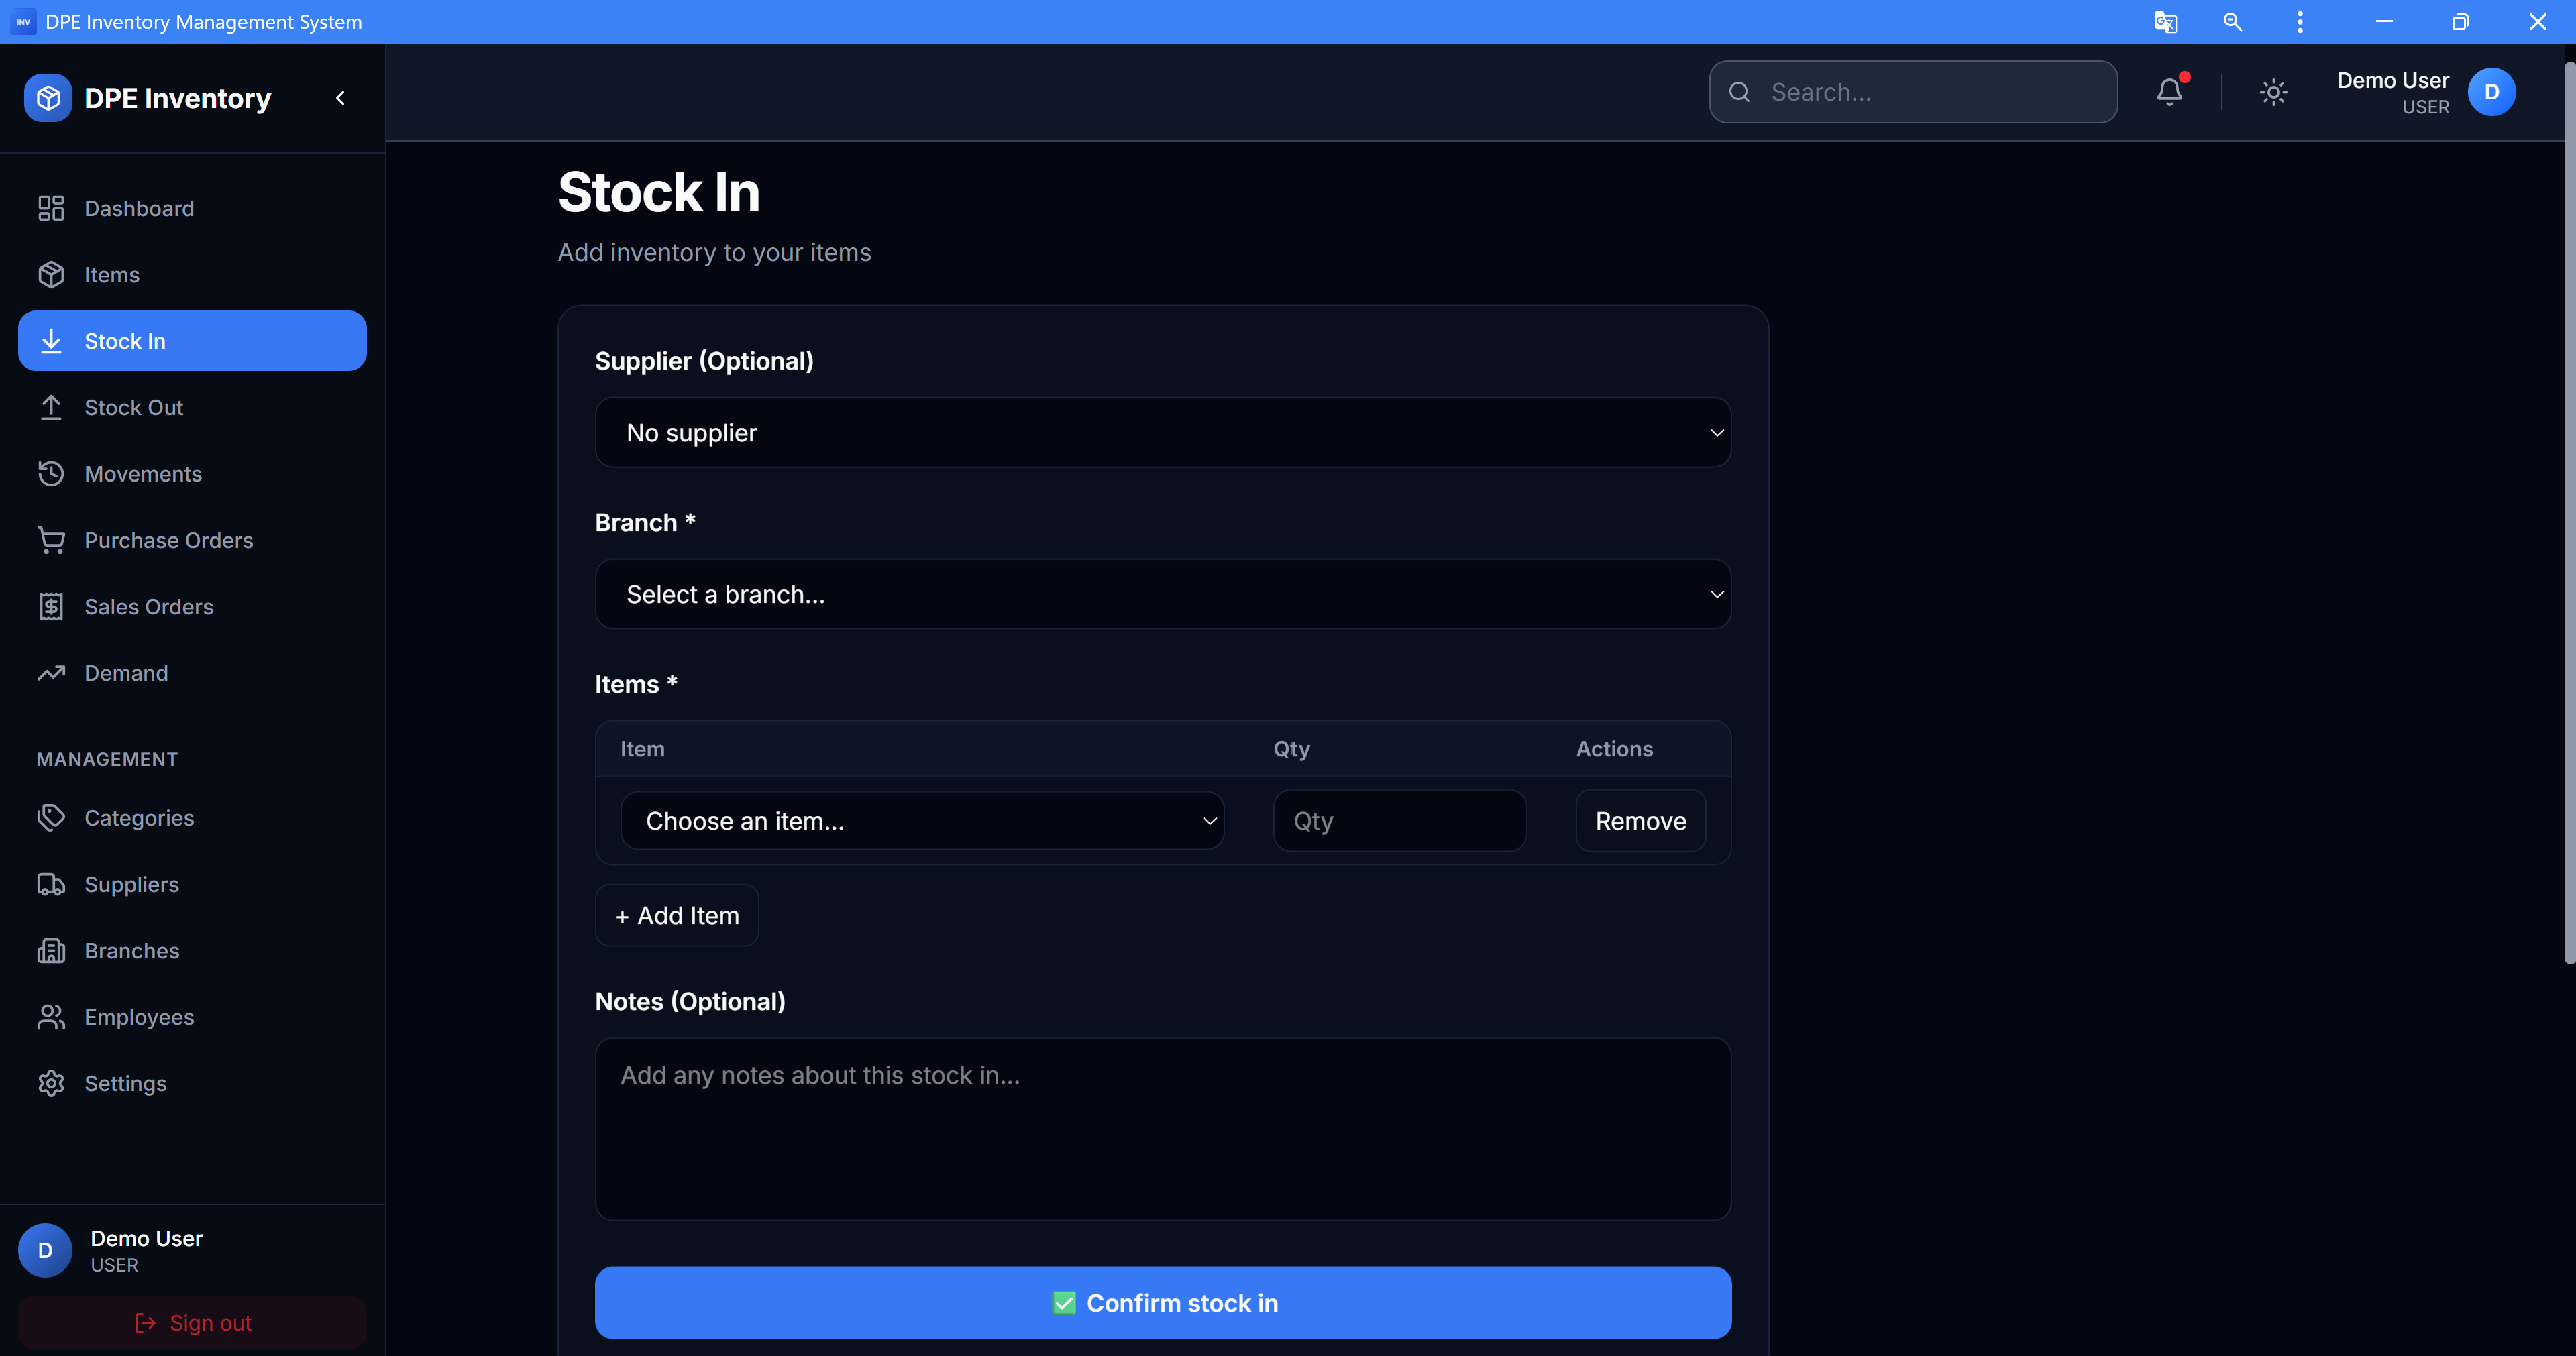
\includegraphics[width=3.6cm, height=2cm]{images/stockIn-dashboard.png}};
  \node[font=\tiny\bfseries, color=secondary] at (8.4,-1.2) {Stock In};

  \node[imgframe] at (12.6,0) {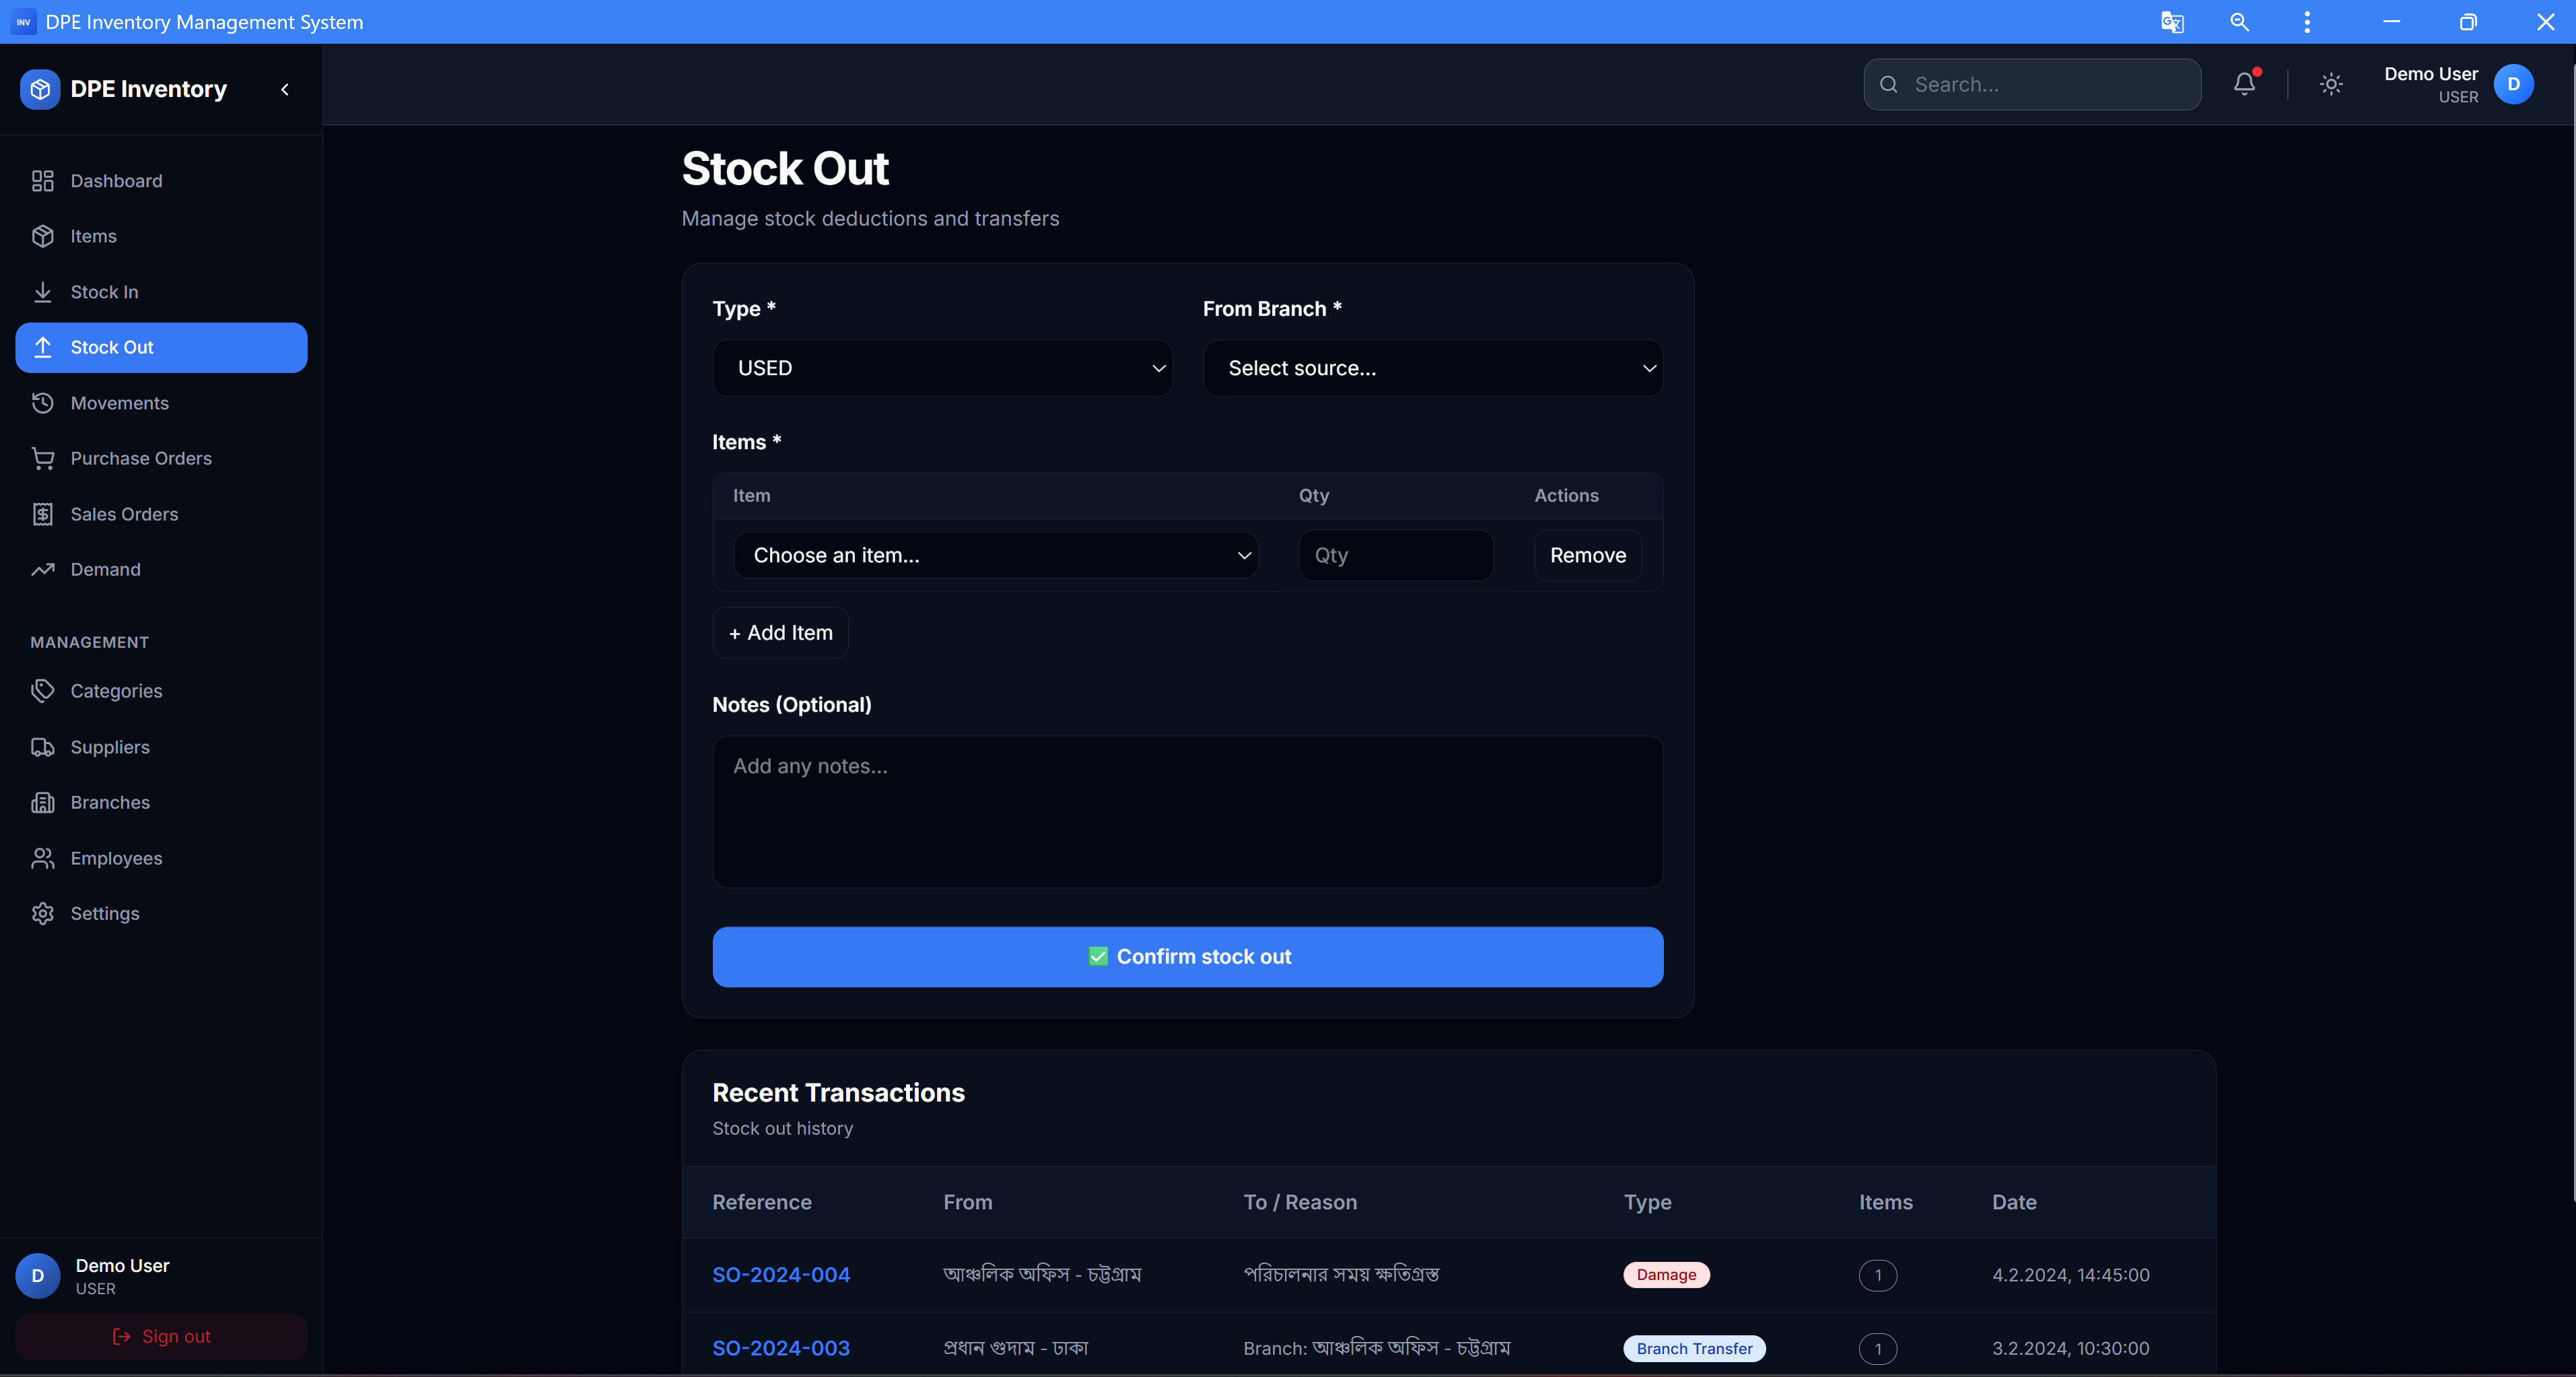
\includegraphics[width=3.6cm, height=2cm]{images/stockOut-dashboard.png}};
  \node[font=\tiny\bfseries, color=secondary] at (12.6,-1.2) {Stock Out};

  % Row 2
  \node[imgframe] at (0,-3) {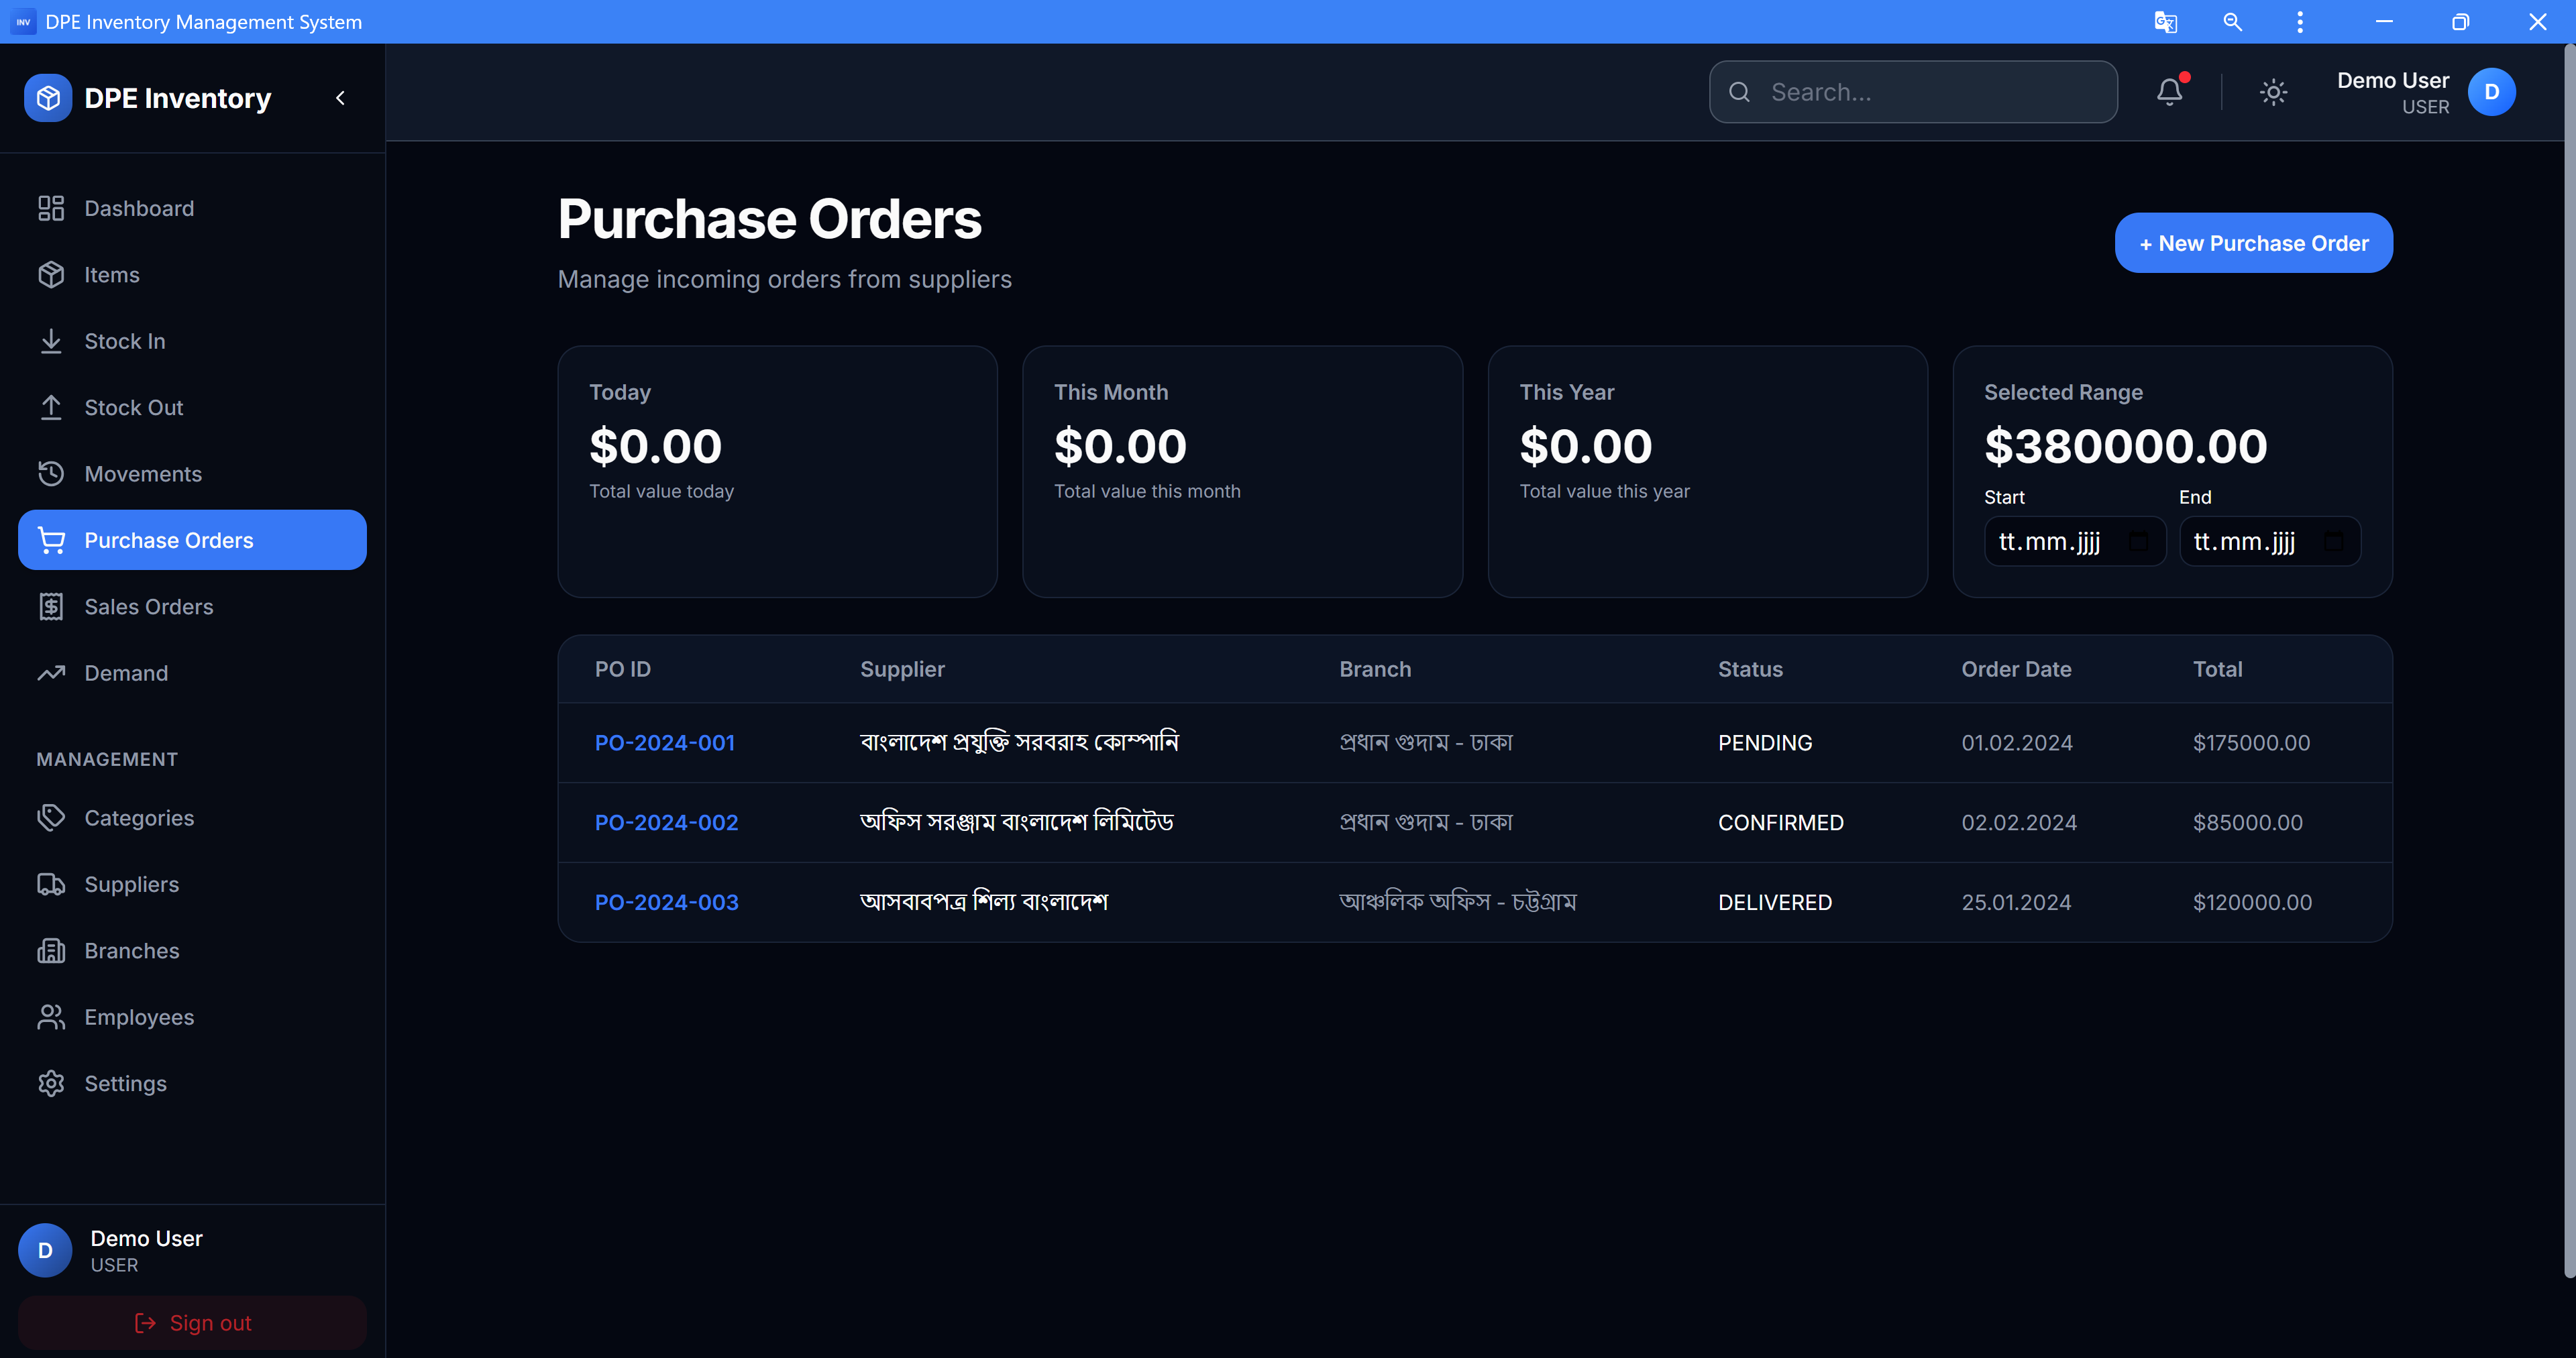
\includegraphics[width=3.6cm, height=2cm]{images/purchase-order-dashboard.png}};
  \node[font=\tiny\bfseries, color=secondary] at (0,-4.2) {Purchase Orders};

  \node[imgframe] at (4.2,-3) {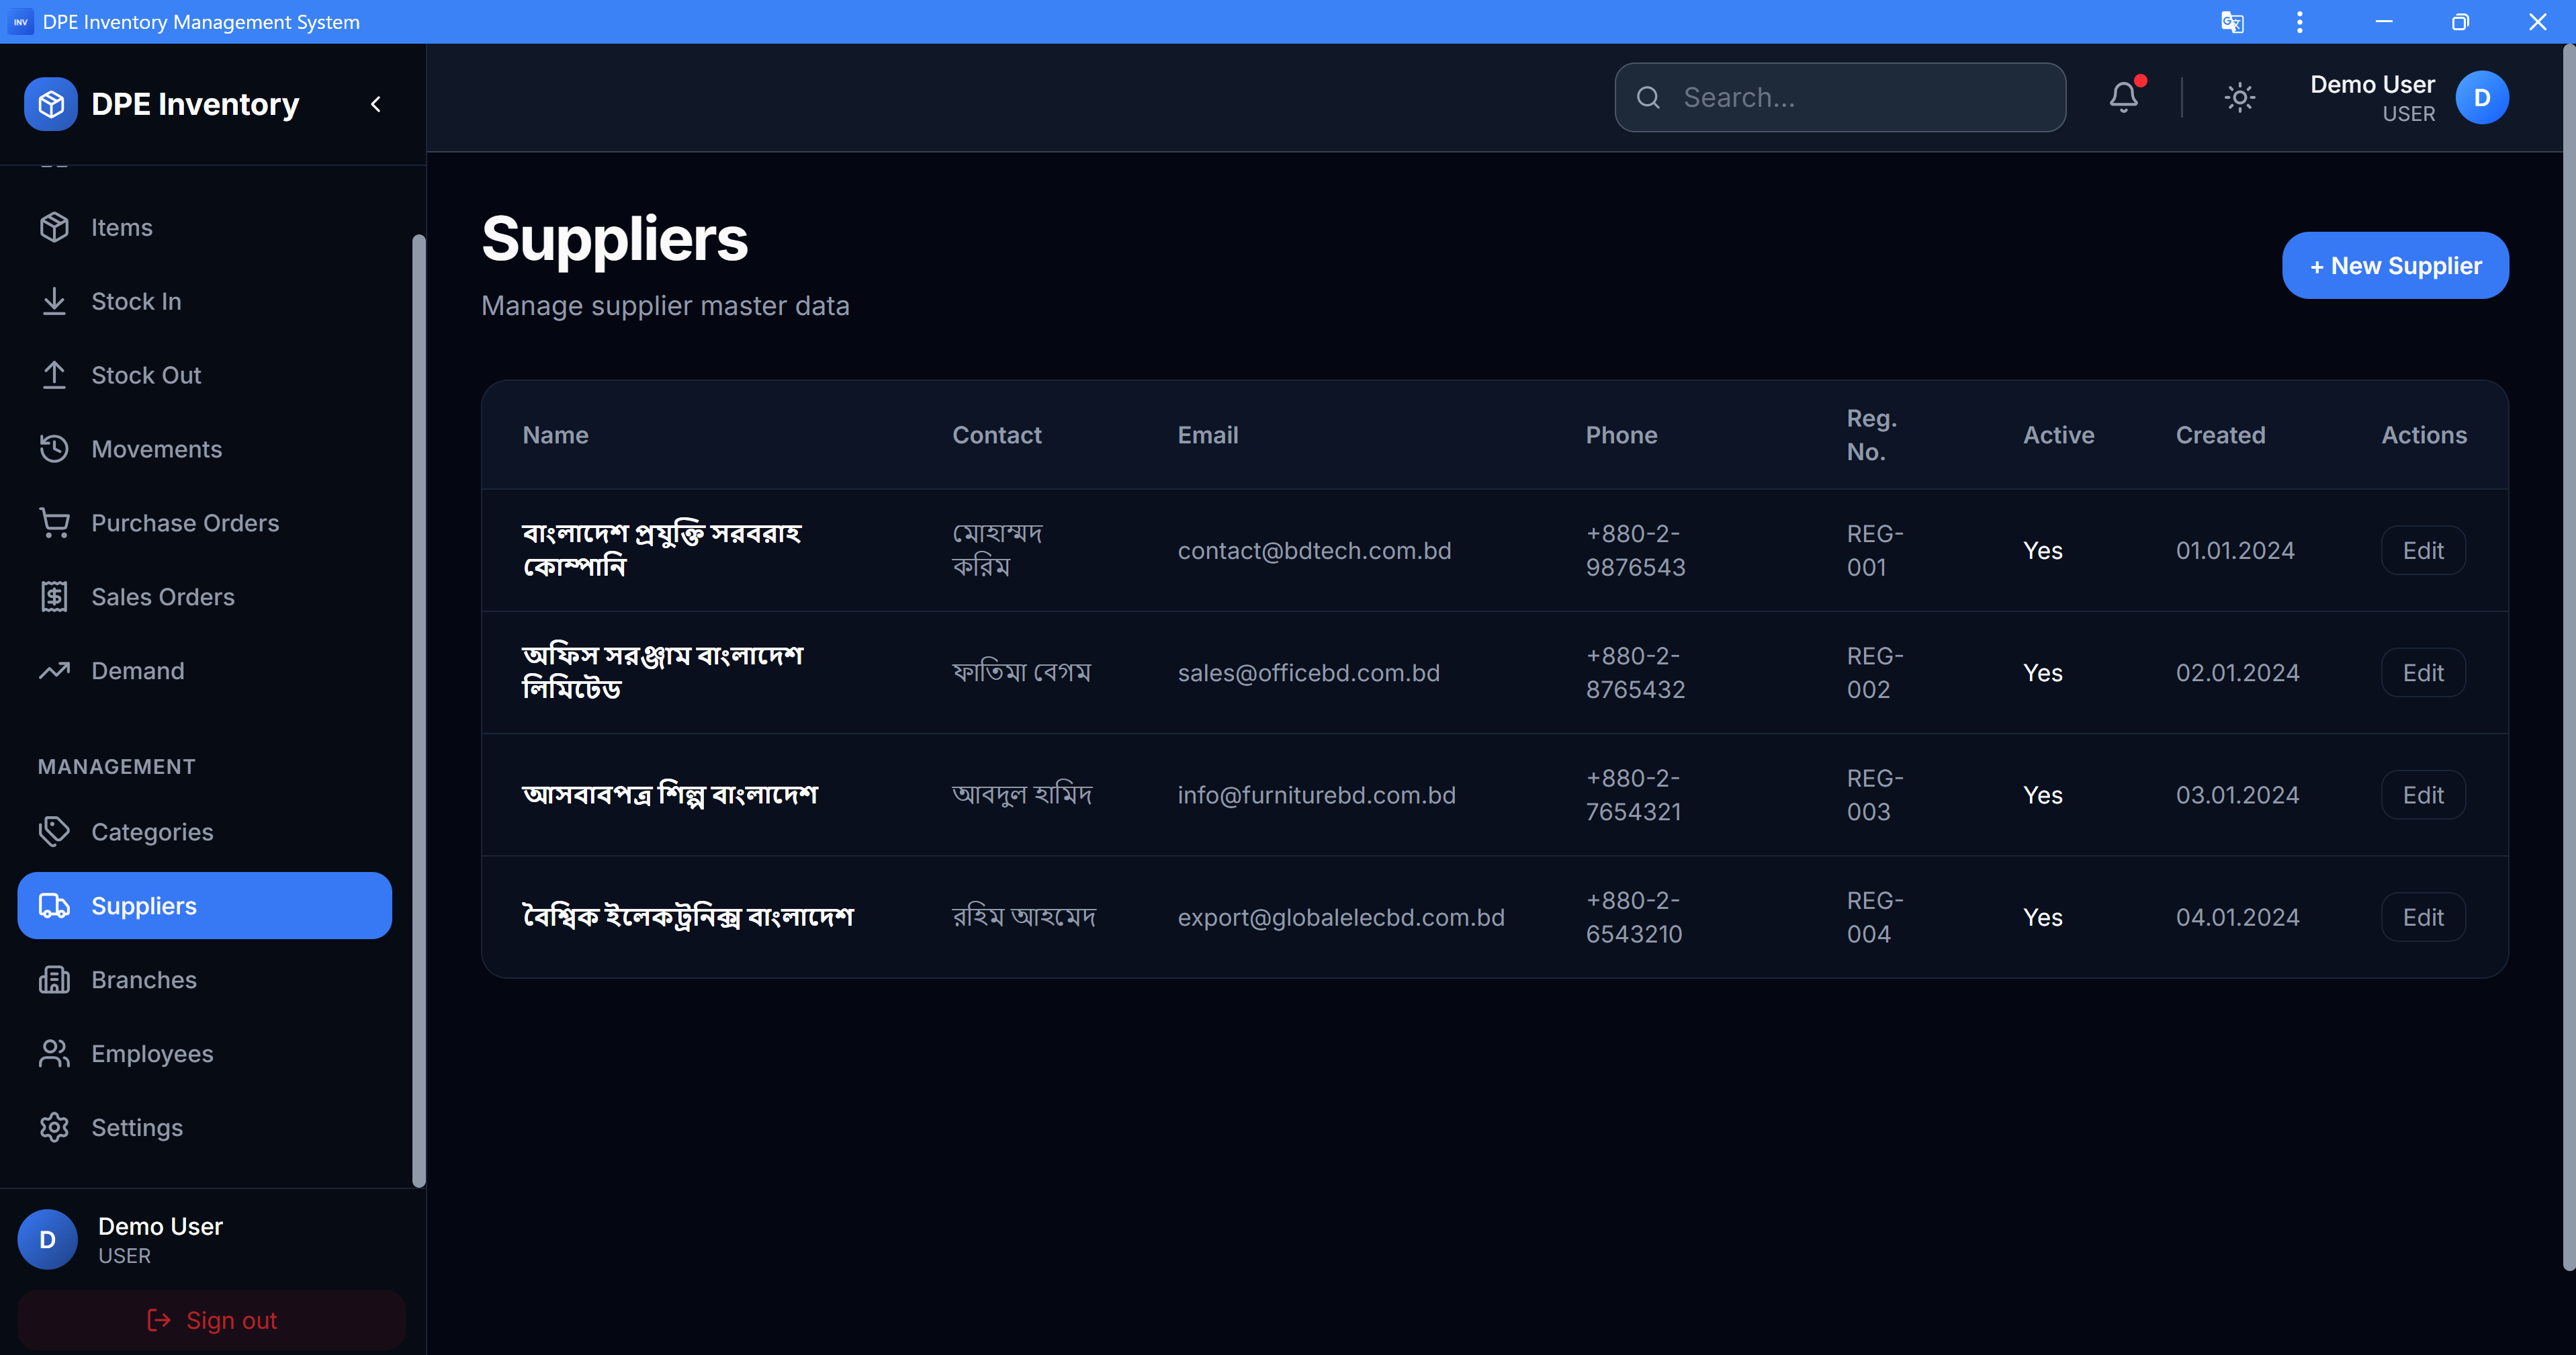
\includegraphics[width=3.6cm, height=2cm]{images/suppliers-dashboard.png}};
  \node[font=\tiny\bfseries, color=secondary] at (4.2,-4.2) {Suppliers};

  \node[imgframe] at (8.4,-3) {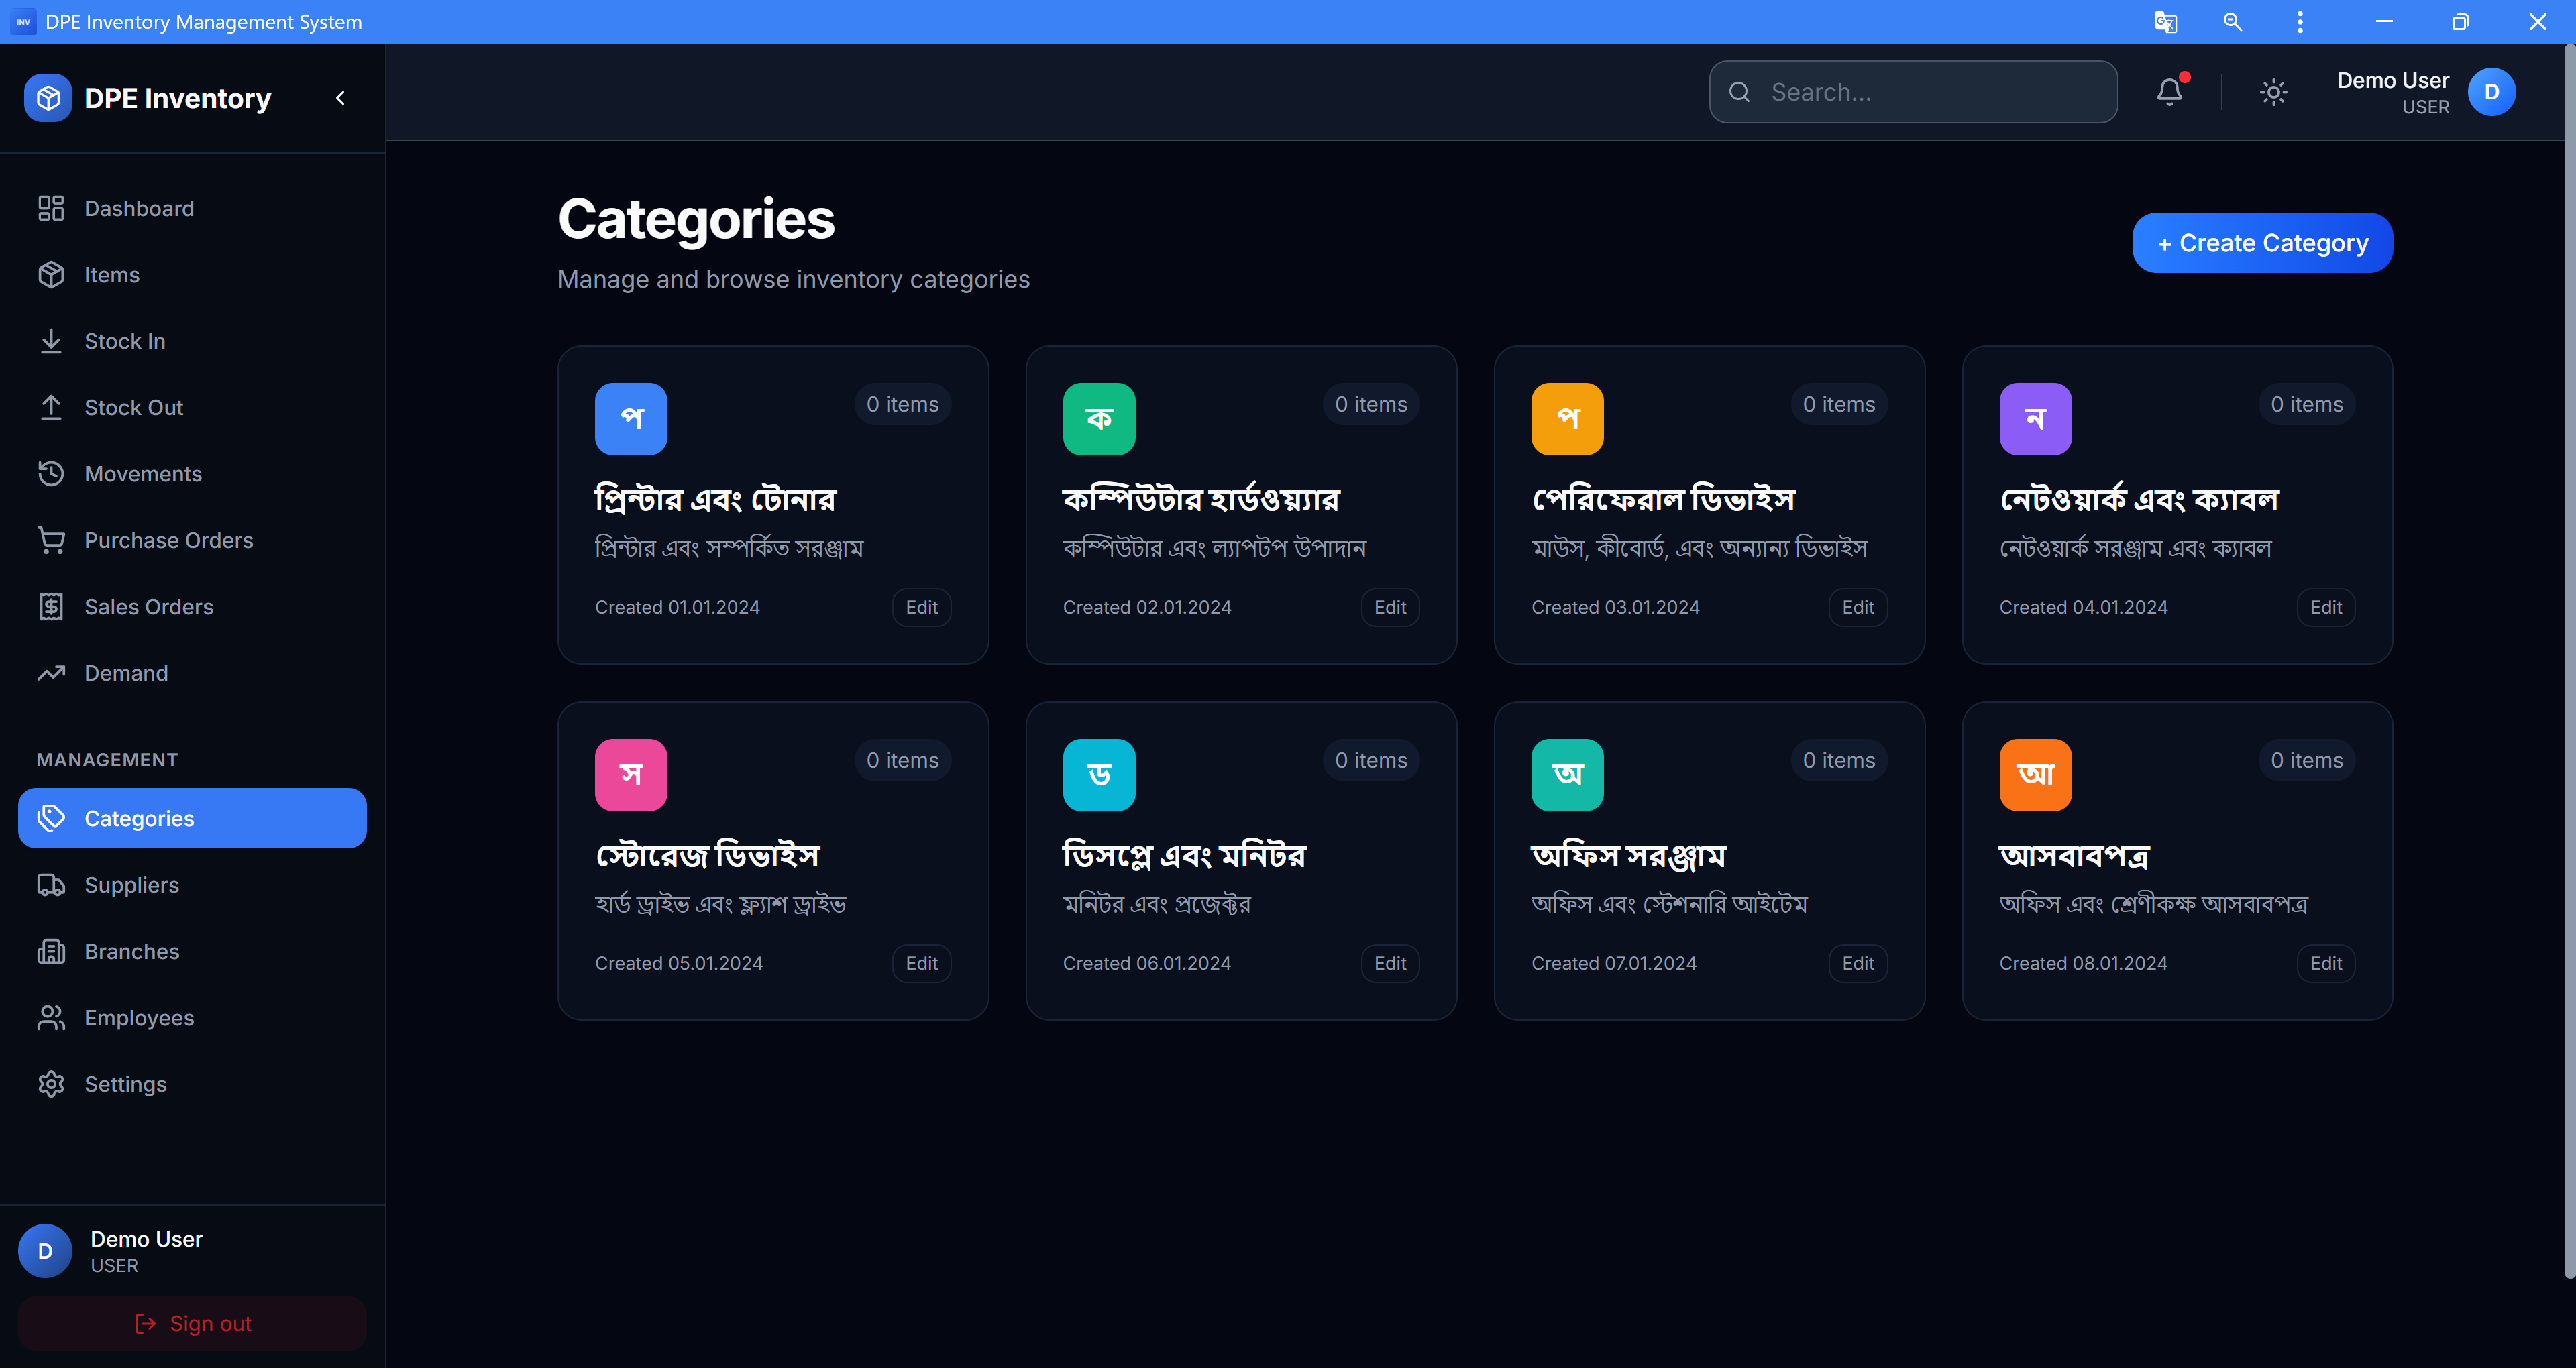
\includegraphics[width=3.6cm, height=2cm]{images/categories-dashboard.png}};
  \node[font=\tiny\bfseries, color=secondary] at (8.4,-4.2) {Categories};

  \node[imgframe] at (12.6,-3) {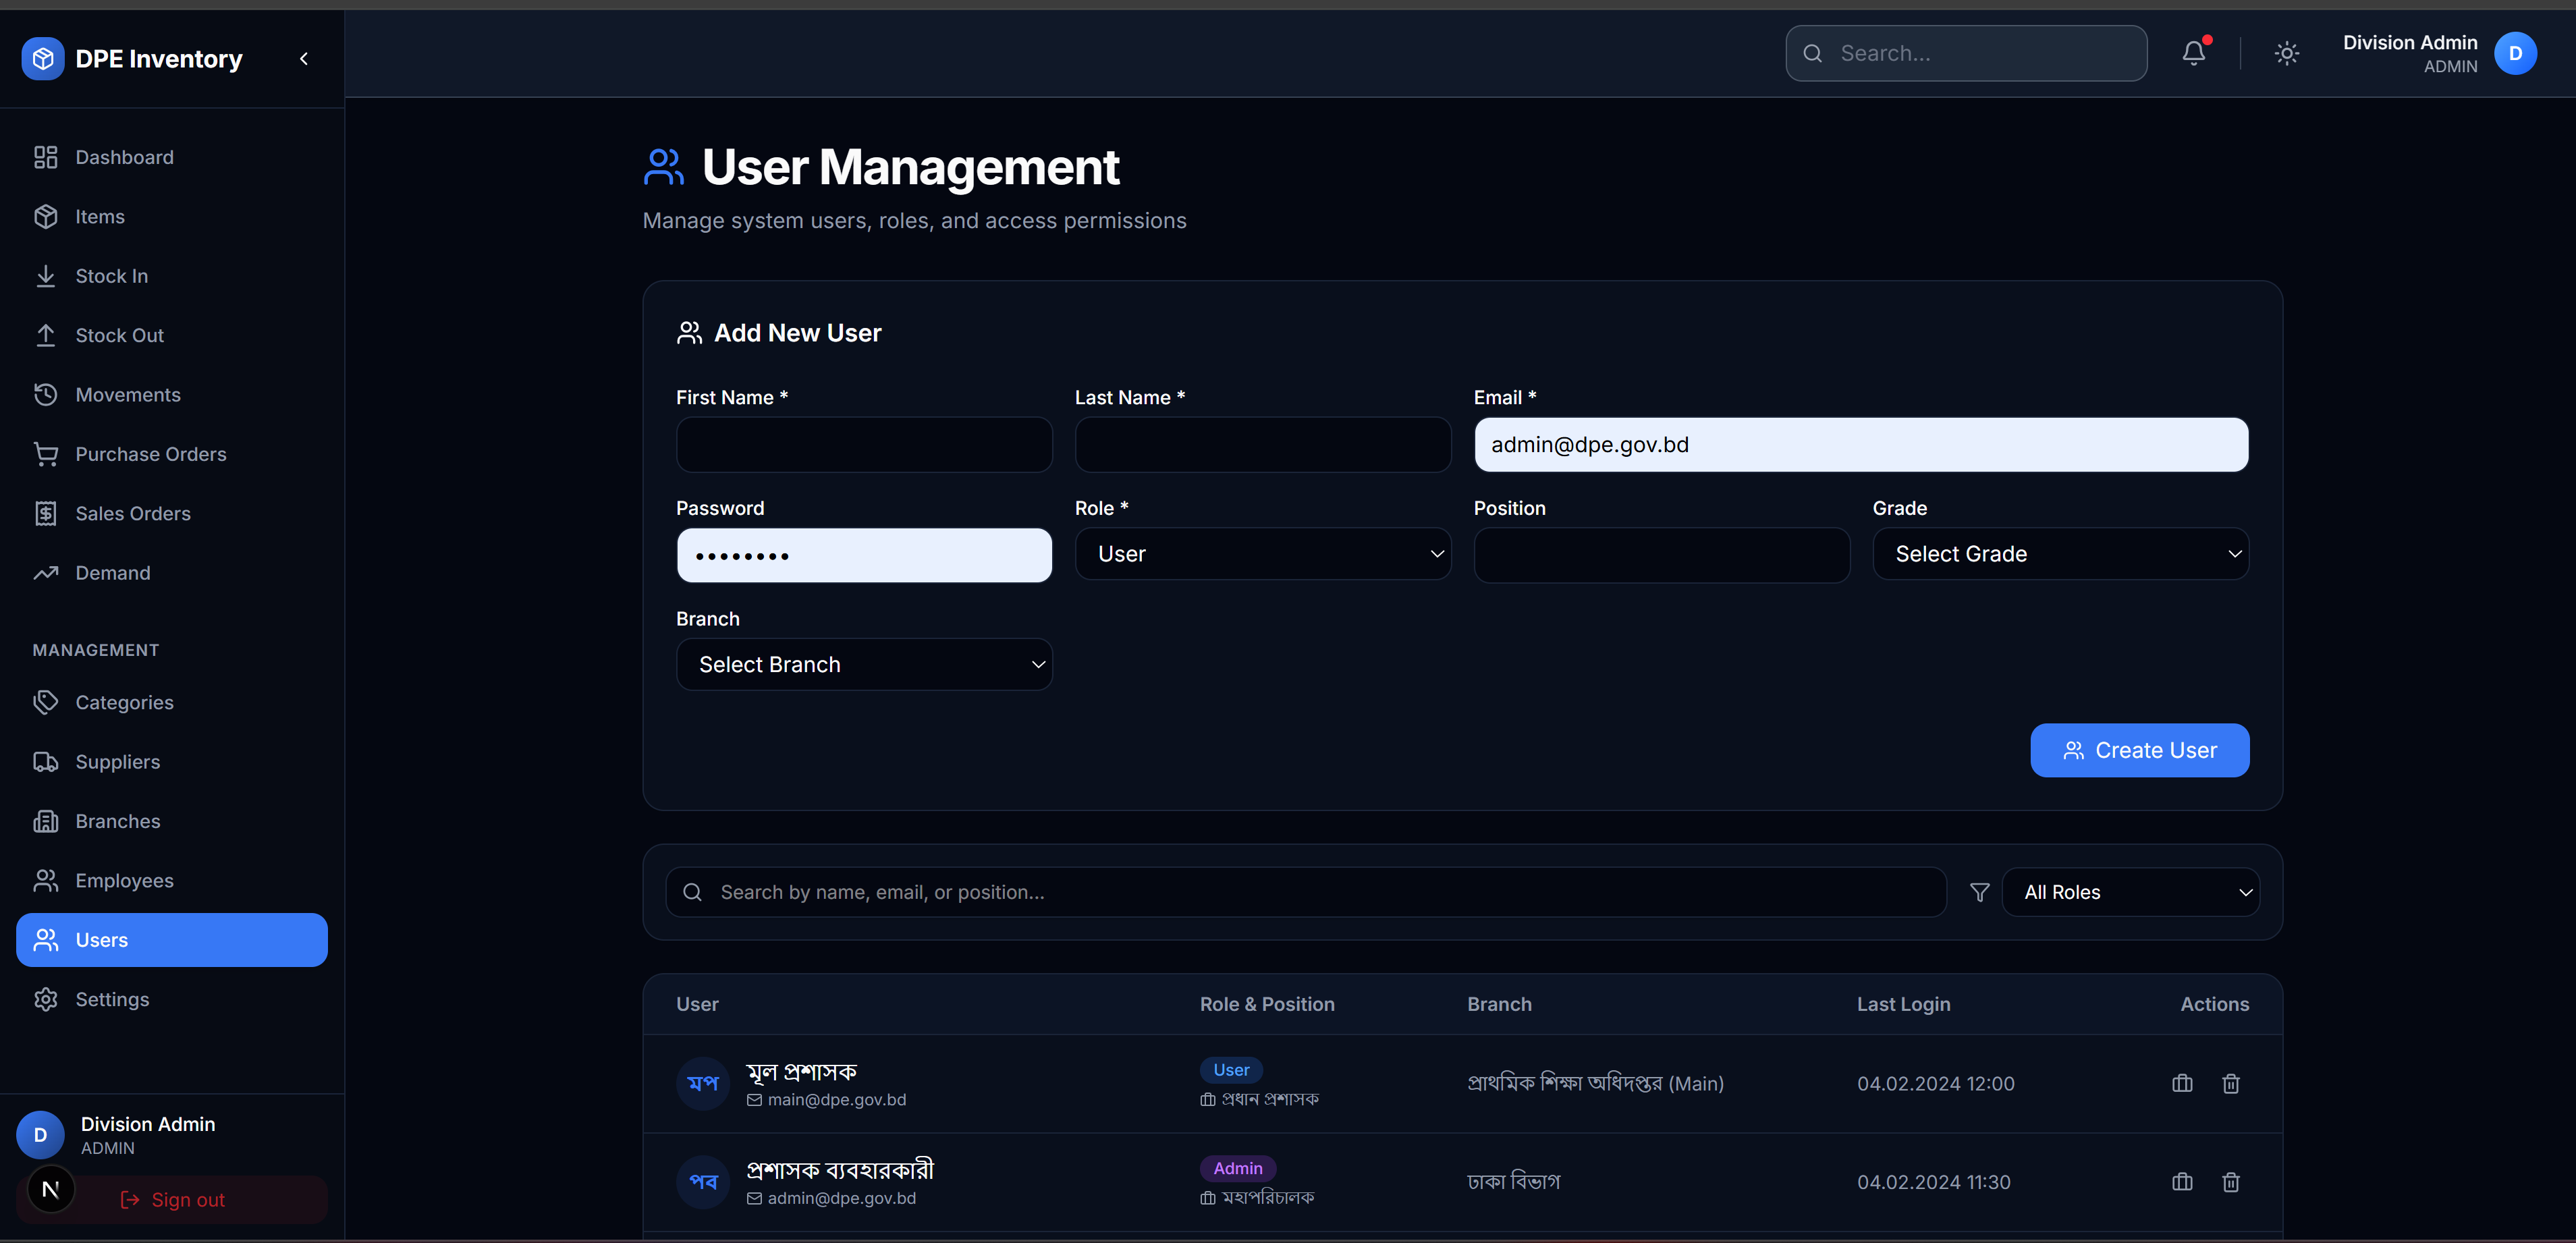
\includegraphics[width=3.6cm, height=2cm]{images/user-managements.png}};
  \node[font=\tiny\bfseries, color=secondary] at (12.6,-4.2) {User Management};
\end{tikzpicture}
\end{center}
\end{frame}

% ===================================================================
% SLIDE 14 — LIVE DEMO URL
% ===================================================================
\begin{frame}{Live System Demo}
\begin{center}
\vspace{0.5cm}
\begin{tikzpicture}
  \node[rounded corners=10pt, fill=primary!5, draw=secondary!30, line width=0.5pt,
        inner sep=15pt, minimum width=10cm] {%
    \begin{minipage}{9cm}\centering
      {\color{secondary}\Large\faIcon{globe}~\textbf{Live Demo URL}}\\[12pt]
      \href{https://inventory-frontend-production-35ac.up.railway.app/}{%
        \color{secondary}\underline{\texttt{https://inventory-frontend-production-35ac.up.railway.app/}}%
      }\\[18pt]
      {\color{medgray}\normalsize\faIcon{user-circle}~\textbf{Demo Credentials:}}\\[8pt]
      \begin{tabular}{ll}
        {\color{accent}\faIcon{user-shield}~\textbf{Admin:}} & \texttt{admin@example.com / Admin@123456} \\[4pt]
        {\color{secondary}\faIcon{user}~\textbf{User:}} & \texttt{user@example.com / User@123456} \\
      \end{tabular}
    \end{minipage}
  };
\end{tikzpicture}

\vspace{0.5cm}
{\small\color{medgray}\faIcon{info-circle}~The platform is fully functional with real-time data — try creating requisitions, viewing stock, and generating reports.}
\end{center}
\end{frame}

% ===================================================================
% SLIDE 15 — MORE SCREENSHOTS
% ===================================================================
\begin{frame}{Additional Platform Views}
\begin{center}
\begin{tikzpicture}[
  imgframe/.style={rounded corners=4pt, draw=softgray, line width=0.4pt, inner sep=0pt,
    drop shadow={shadow xshift=0.5pt, shadow yshift=-0.5pt, opacity=0.06}}
]
  \node[imgframe] at (0,0) {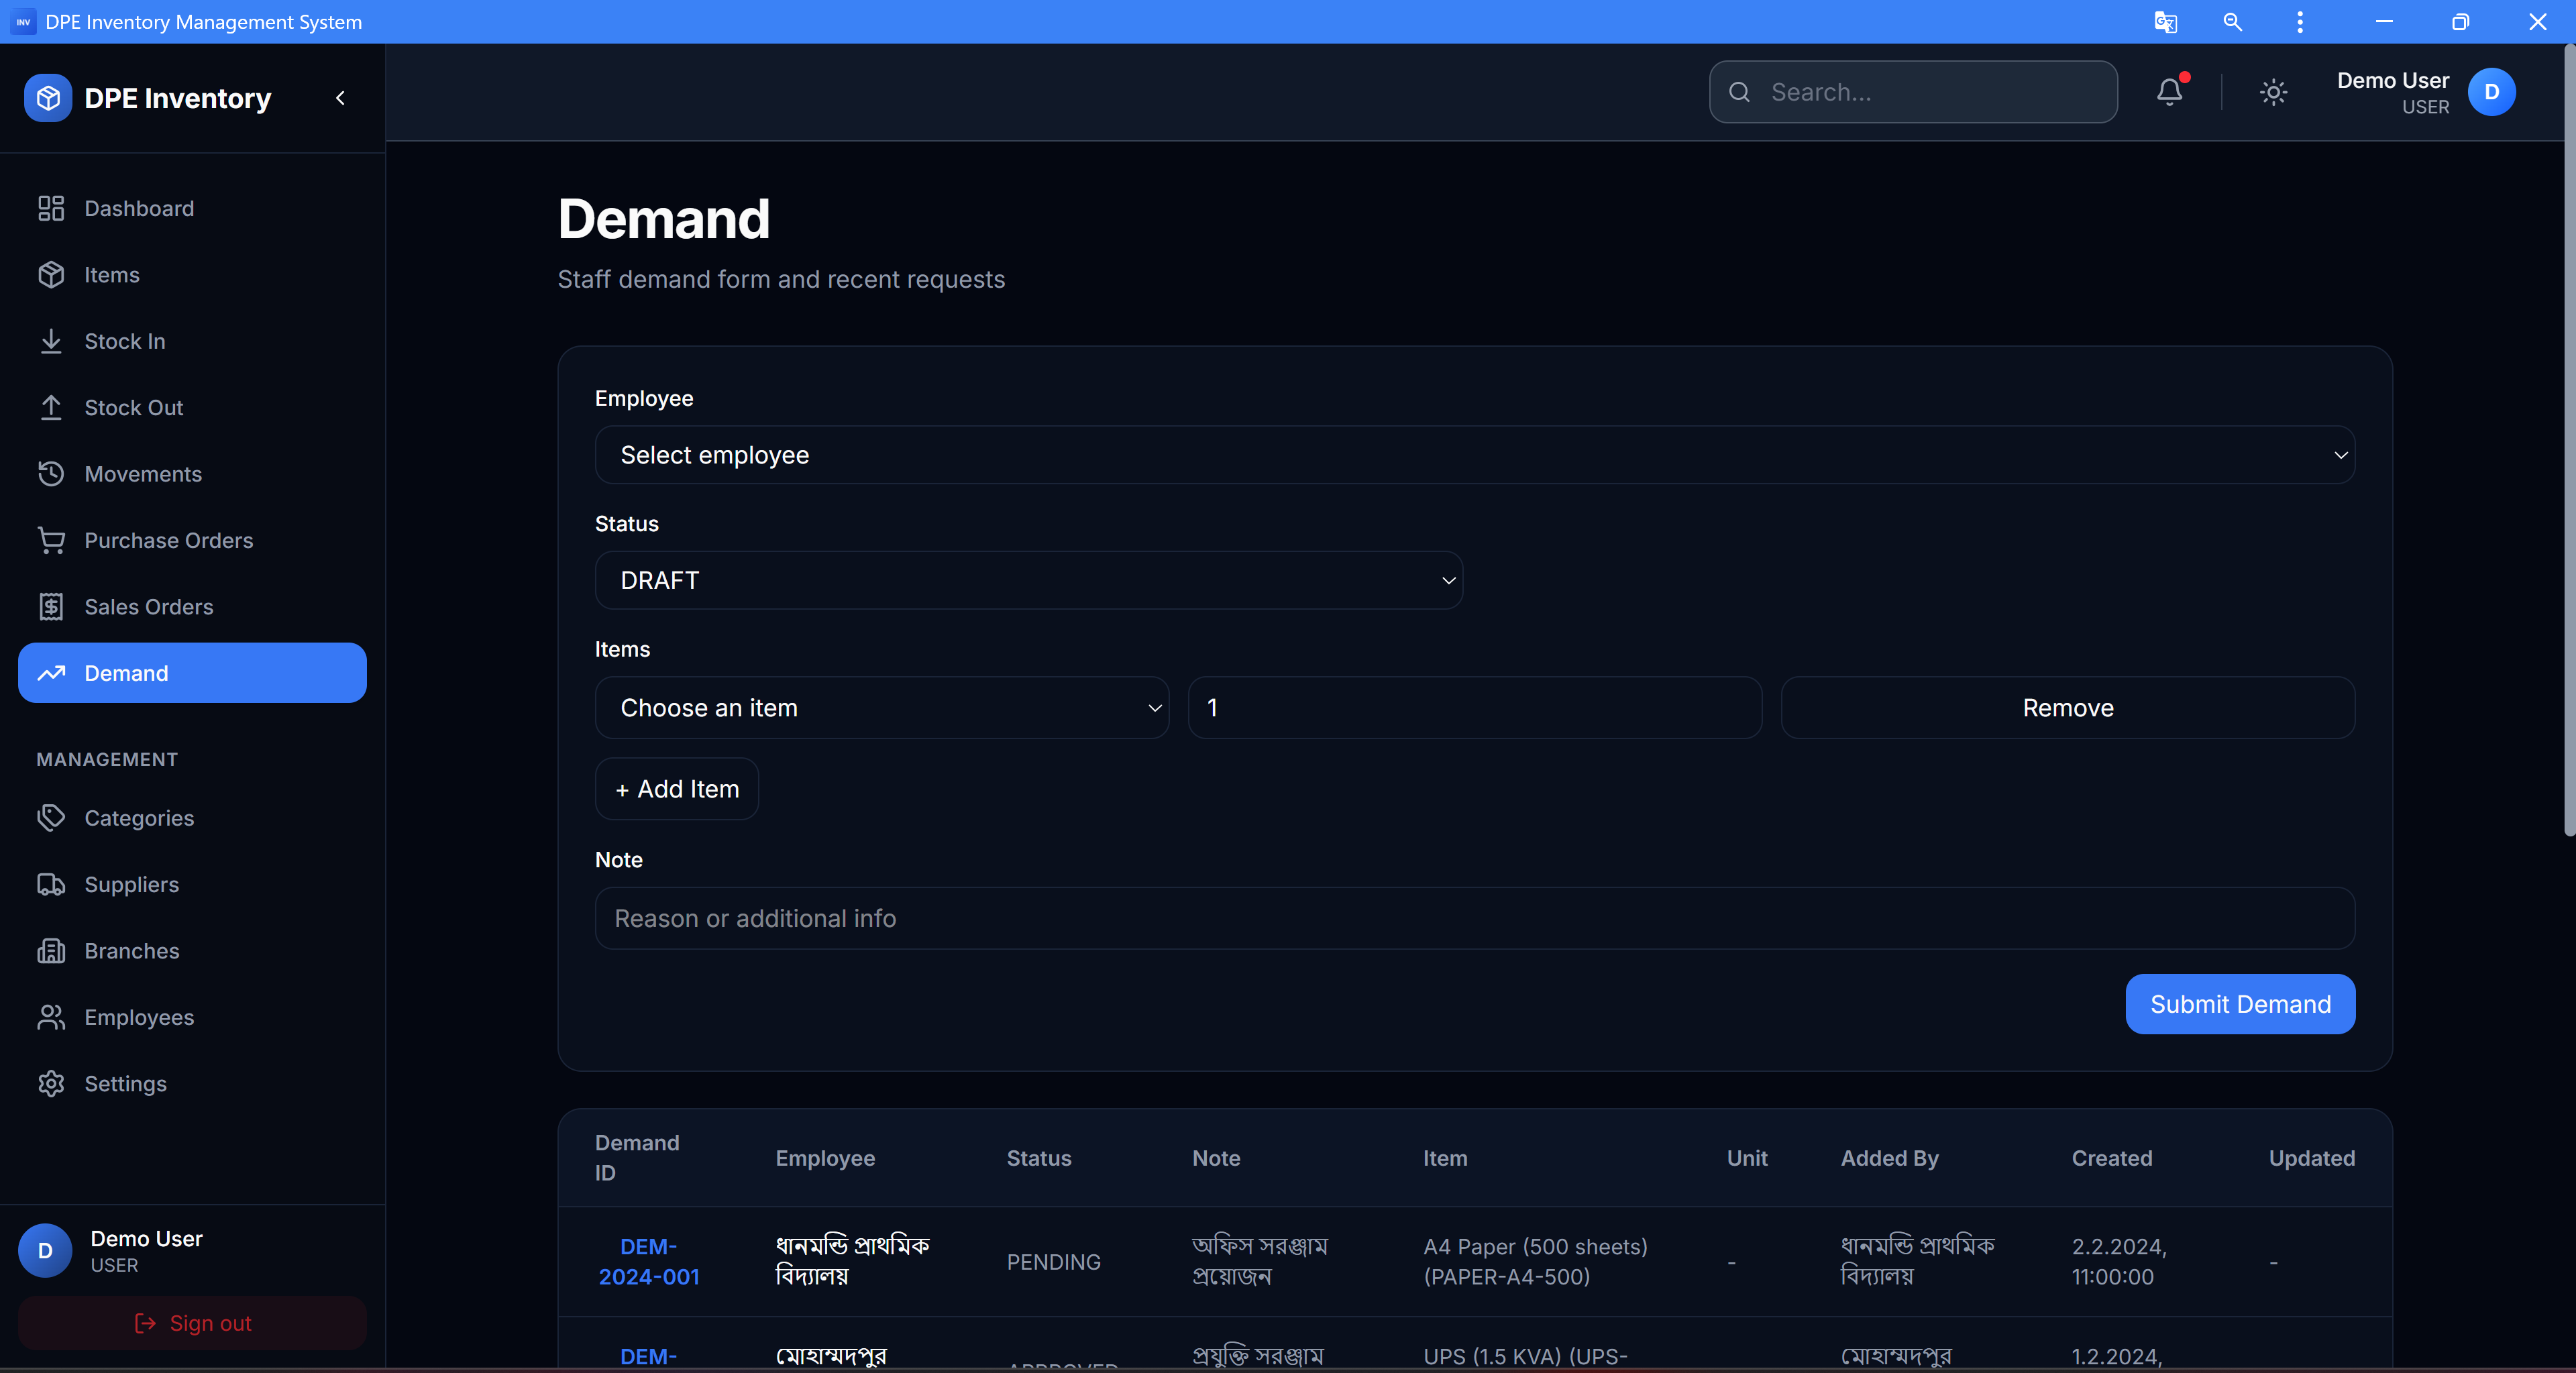
\includegraphics[width=3.6cm, height=2cm]{images/demand-dashboard.png}};
  \node[font=\tiny\bfseries, color=secondary] at (0,-1.2) {Demand Forecasting};

  \node[imgframe] at (4.2,0) {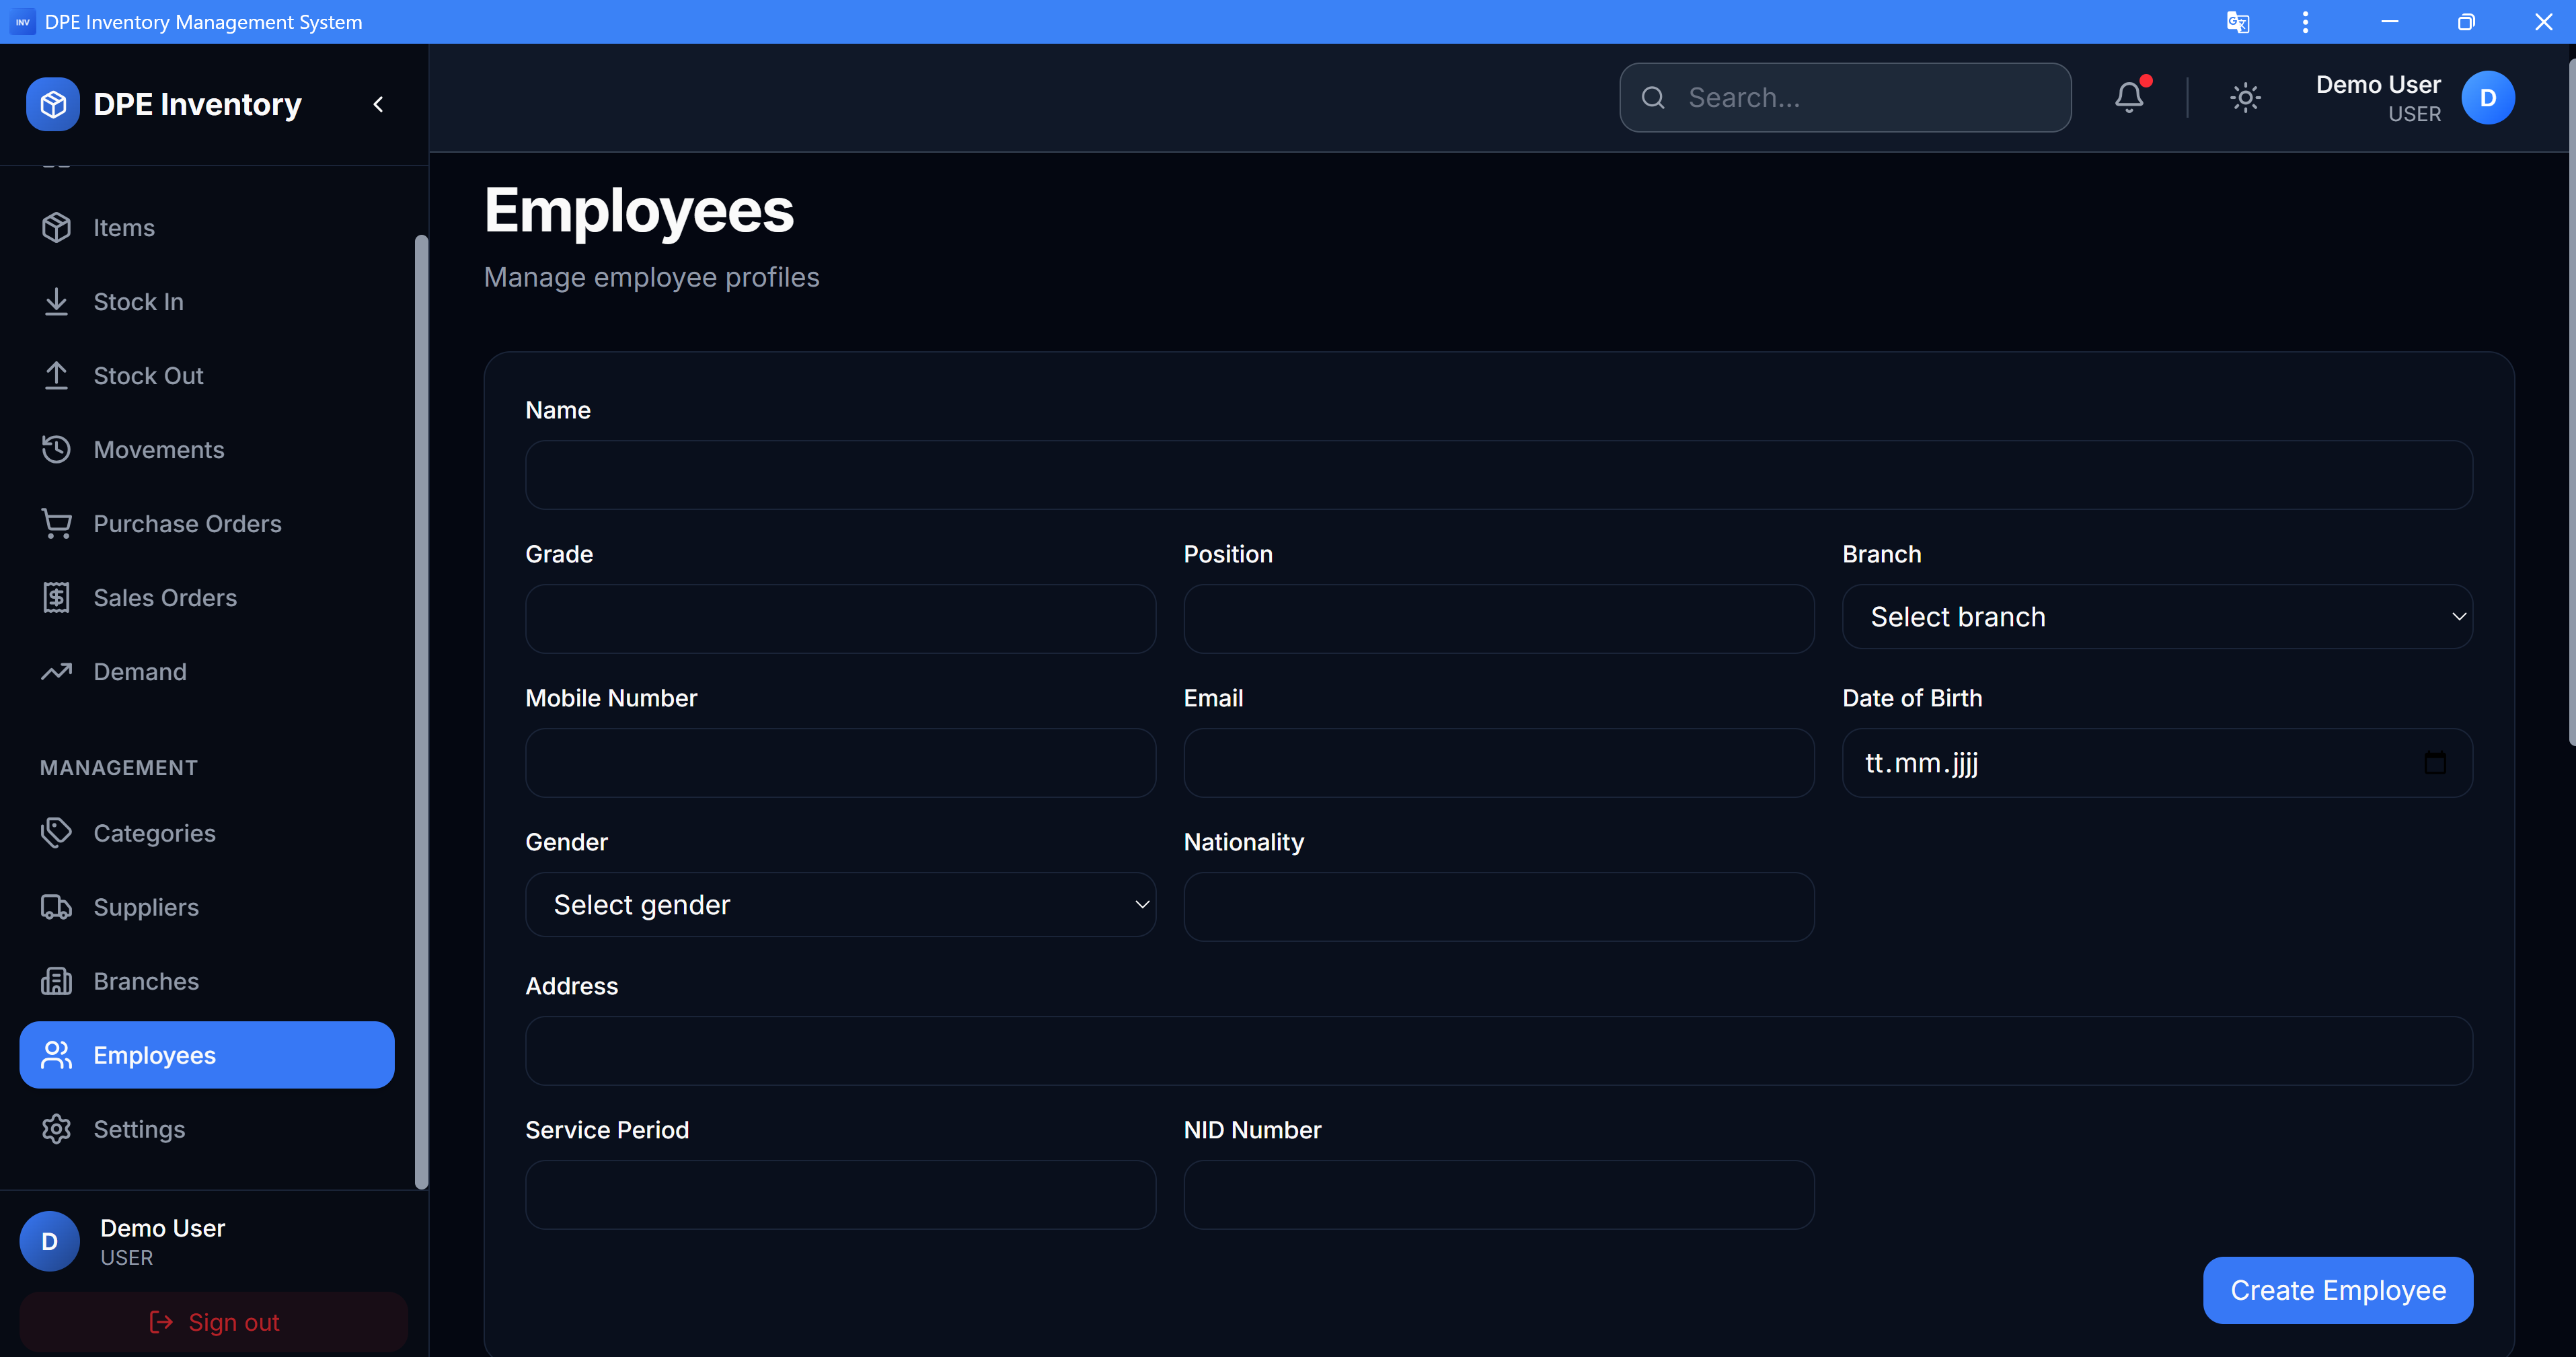
\includegraphics[width=3.6cm, height=2cm]{images/employees-dashboard.png}};
  \node[font=\tiny\bfseries, color=secondary] at (4.2,-1.2) {Employee Management};

  \node[imgframe] at (8.4,0) {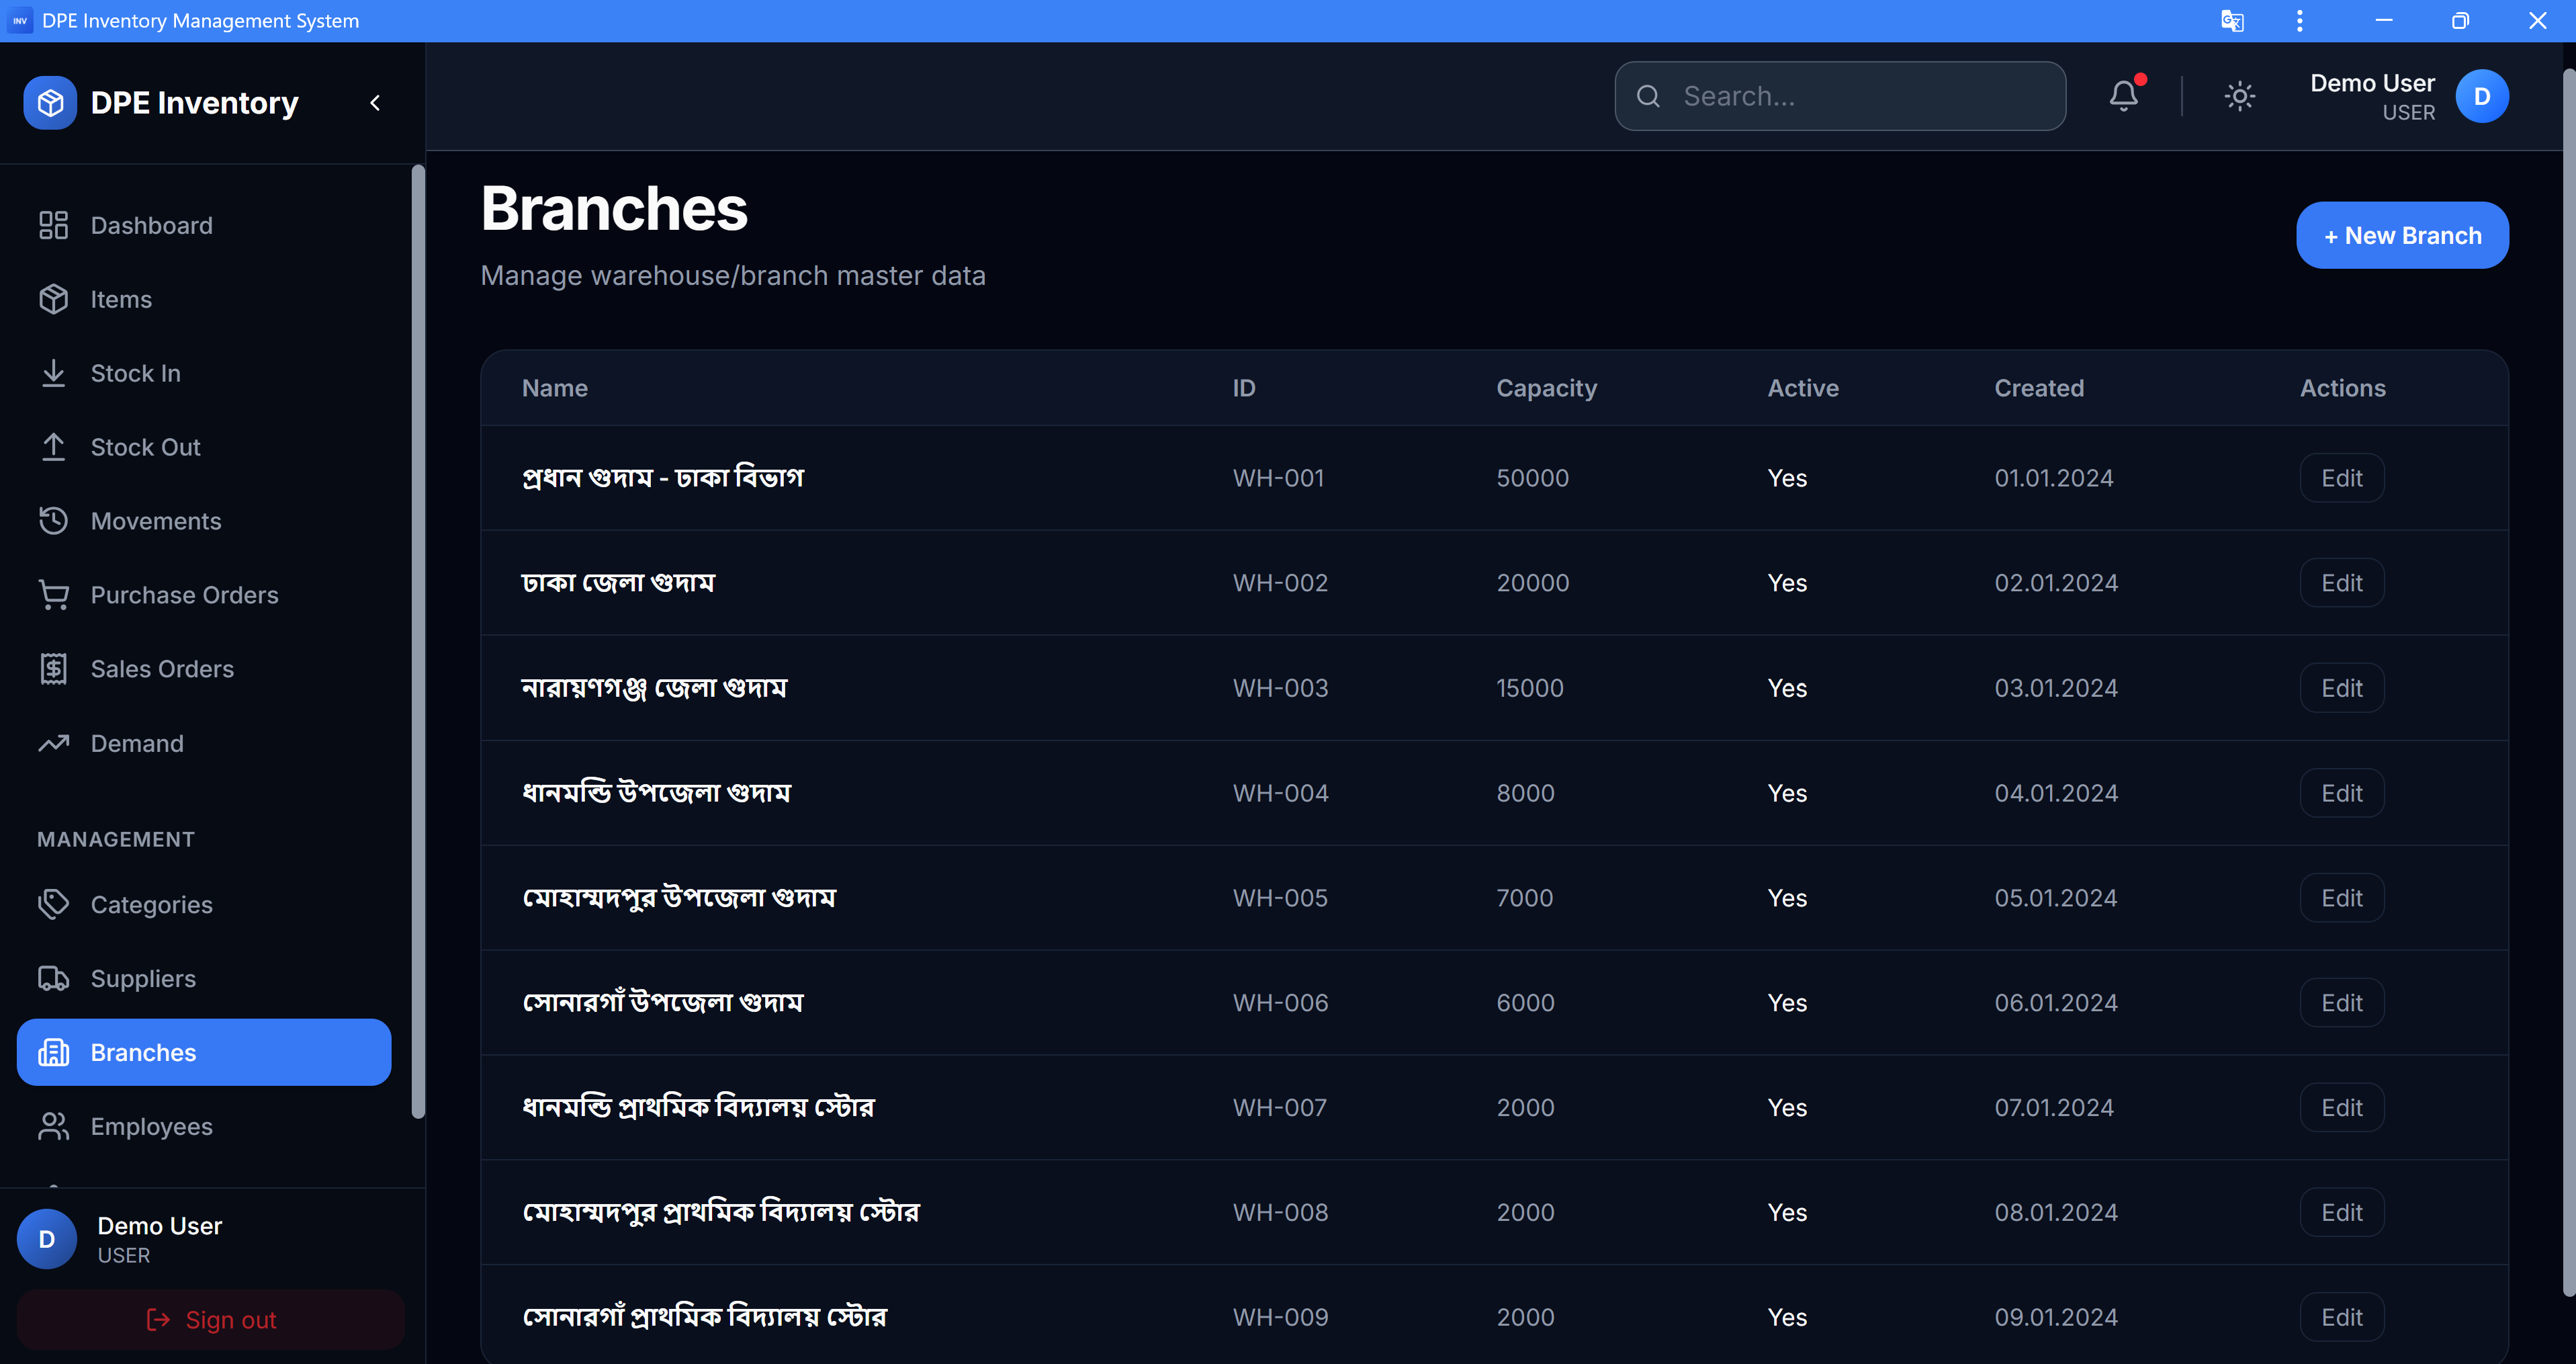
\includegraphics[width=3.6cm, height=2cm]{images/branches-dashboard.png}};
  \node[font=\tiny\bfseries, color=secondary] at (8.4,-1.2) {Branch Network};

  \node[imgframe] at (12.6,0) {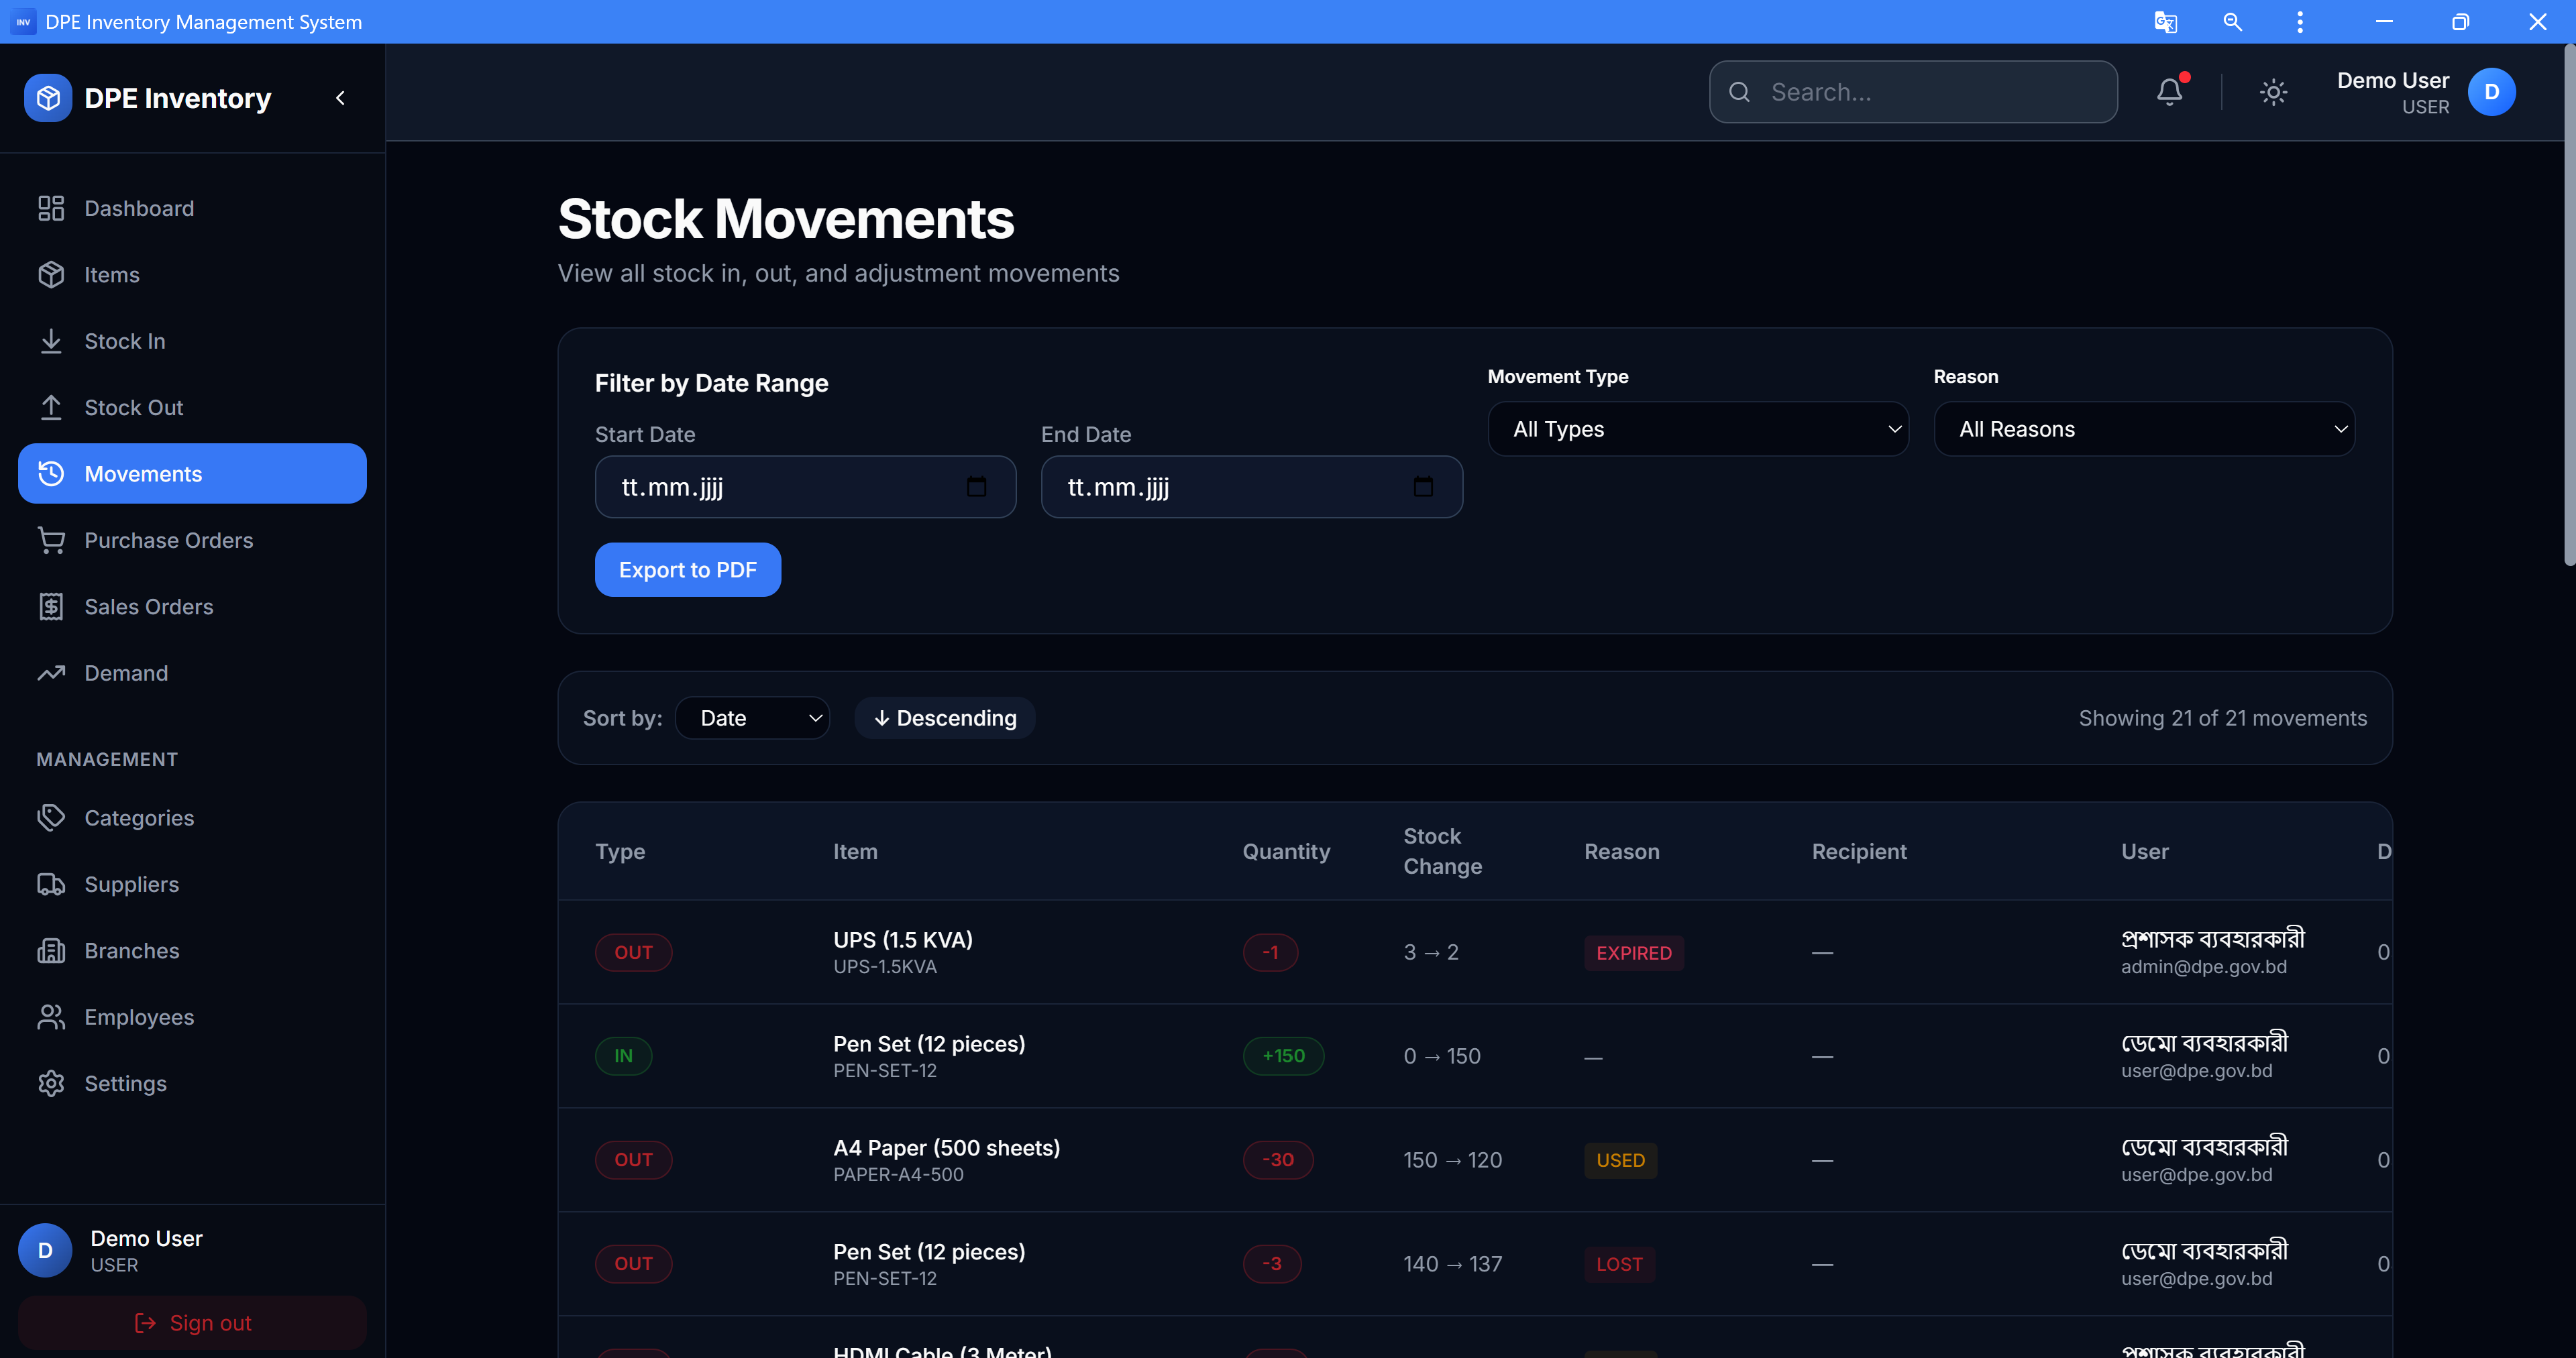
\includegraphics[width=3.6cm, height=2cm]{images/stockOut-report-dashboard.png}};
  \node[font=\tiny\bfseries, color=secondary] at (12.6,-1.2) {Stock Out Reports};

  % Row 2
  \node[imgframe] at (2.1,-3) {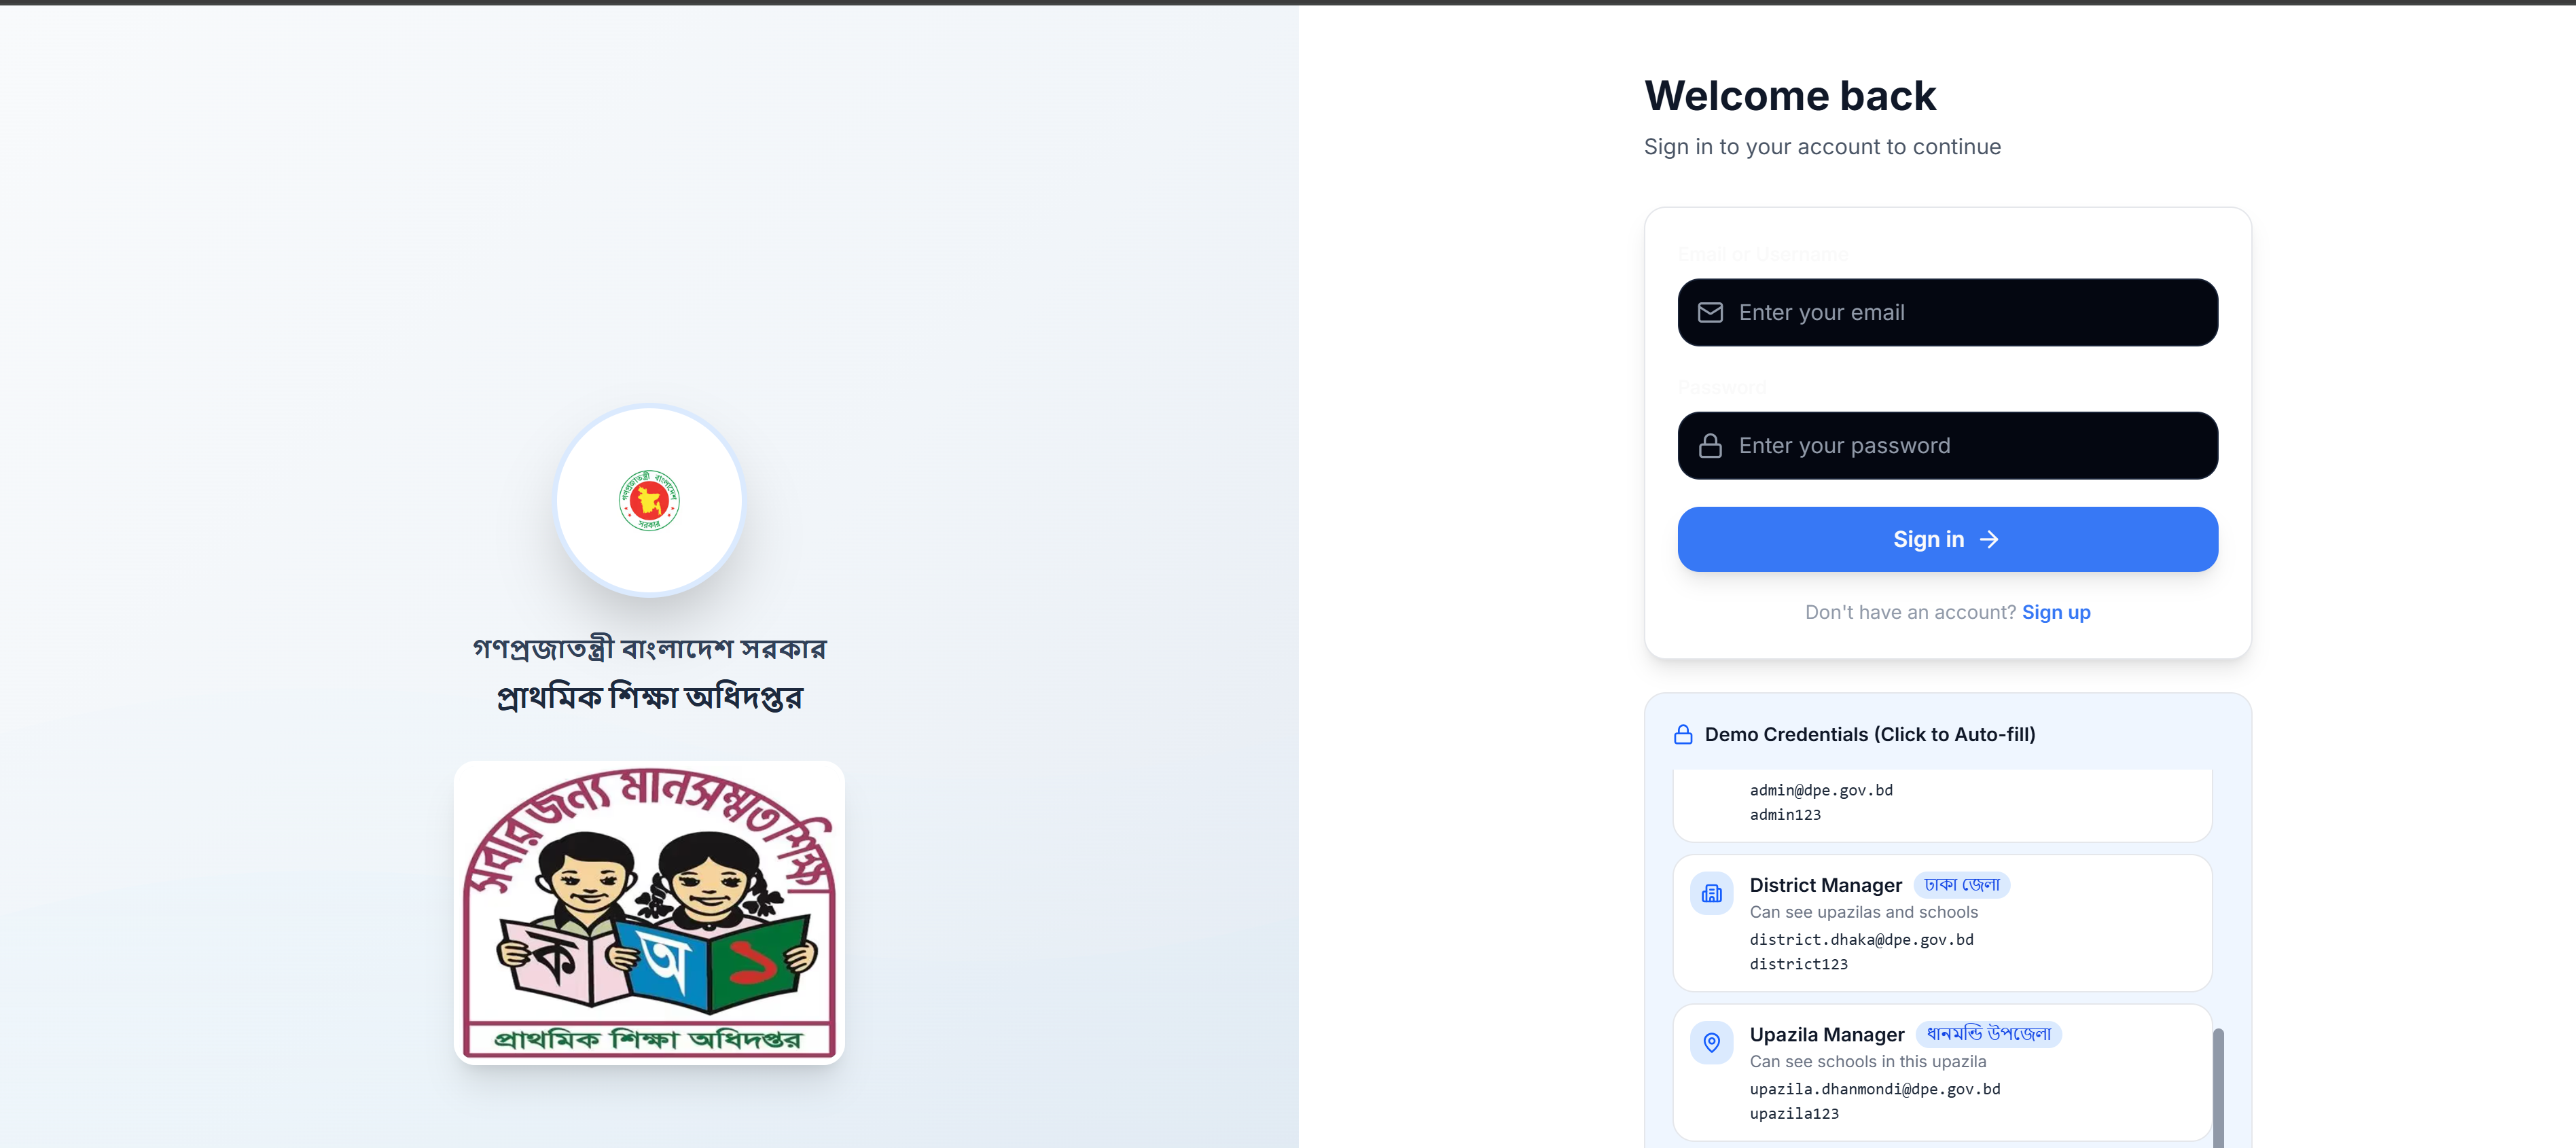
\includegraphics[width=3.6cm, height=2cm]{images/signIn-page.png}};
  \node[font=\tiny\bfseries, color=secondary] at (2.1,-4.2) {Secure Sign-In};

  \node[imgframe] at (6.3,-3) {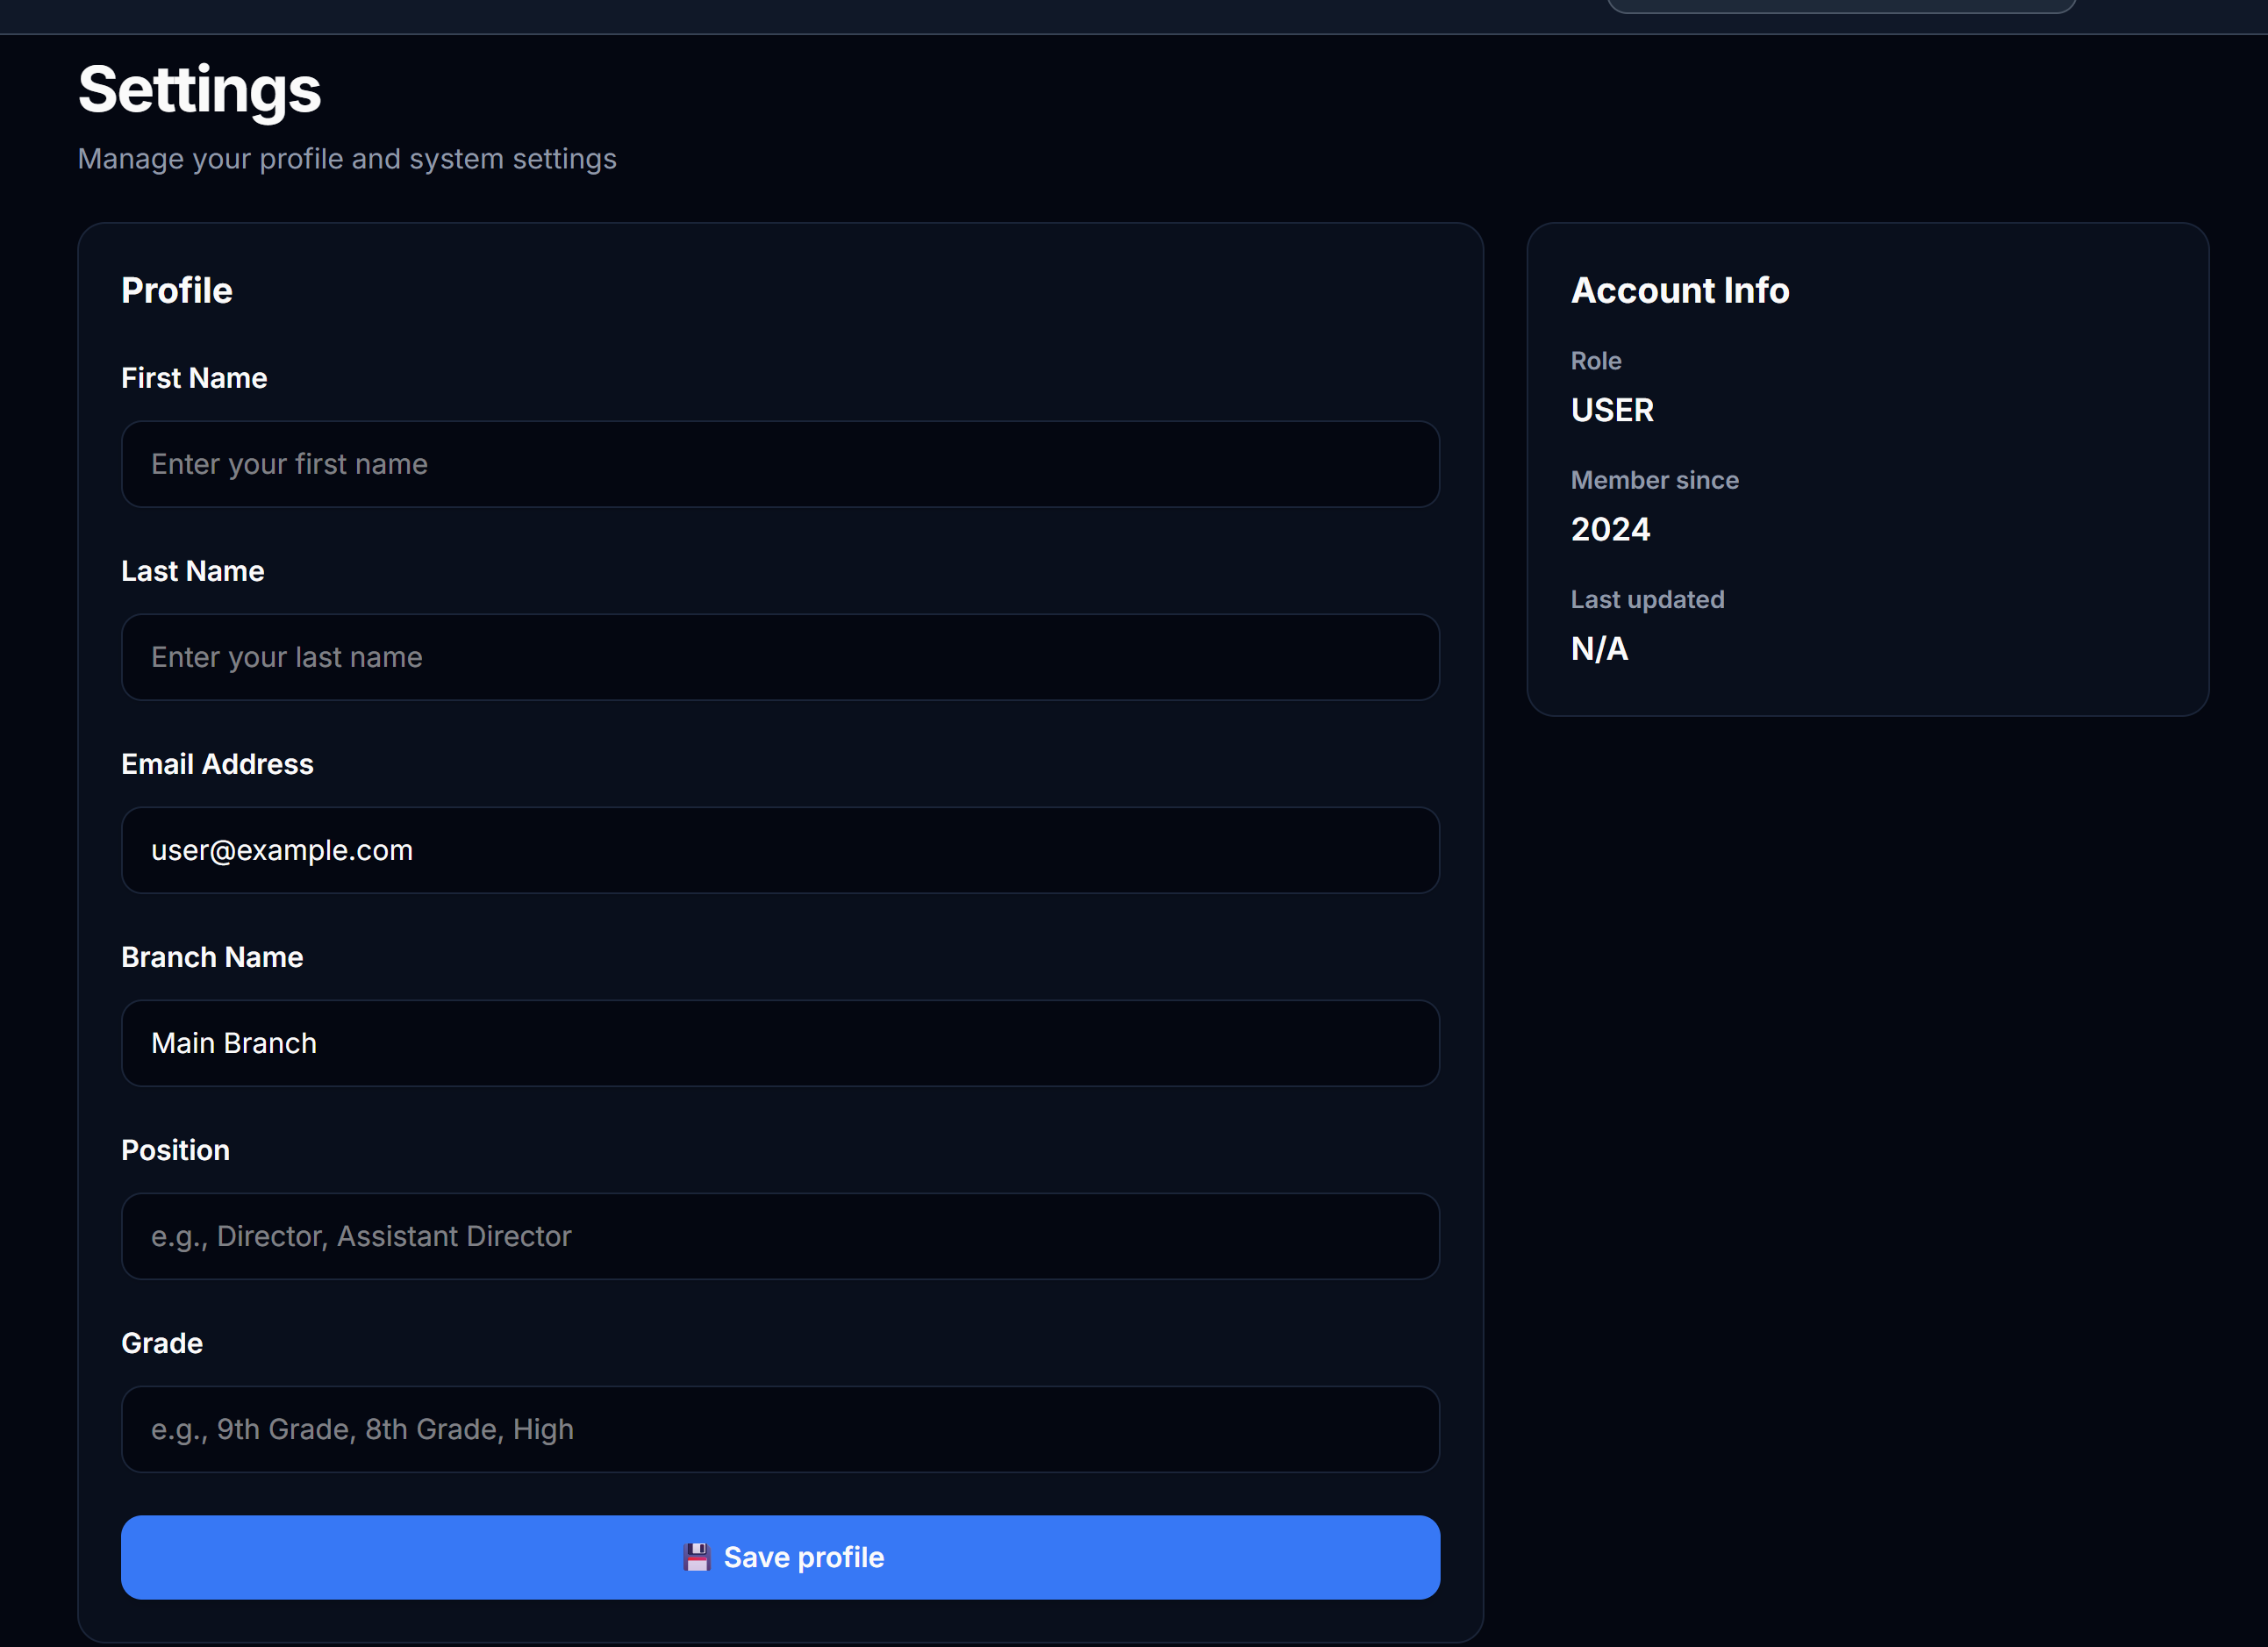
\includegraphics[width=3.6cm, height=2cm]{images/profile-setting.png}};
  \node[font=\tiny\bfseries, color=secondary] at (6.3,-4.2) {Profile Settings};

  \node[imgframe] at (10.5,-3) {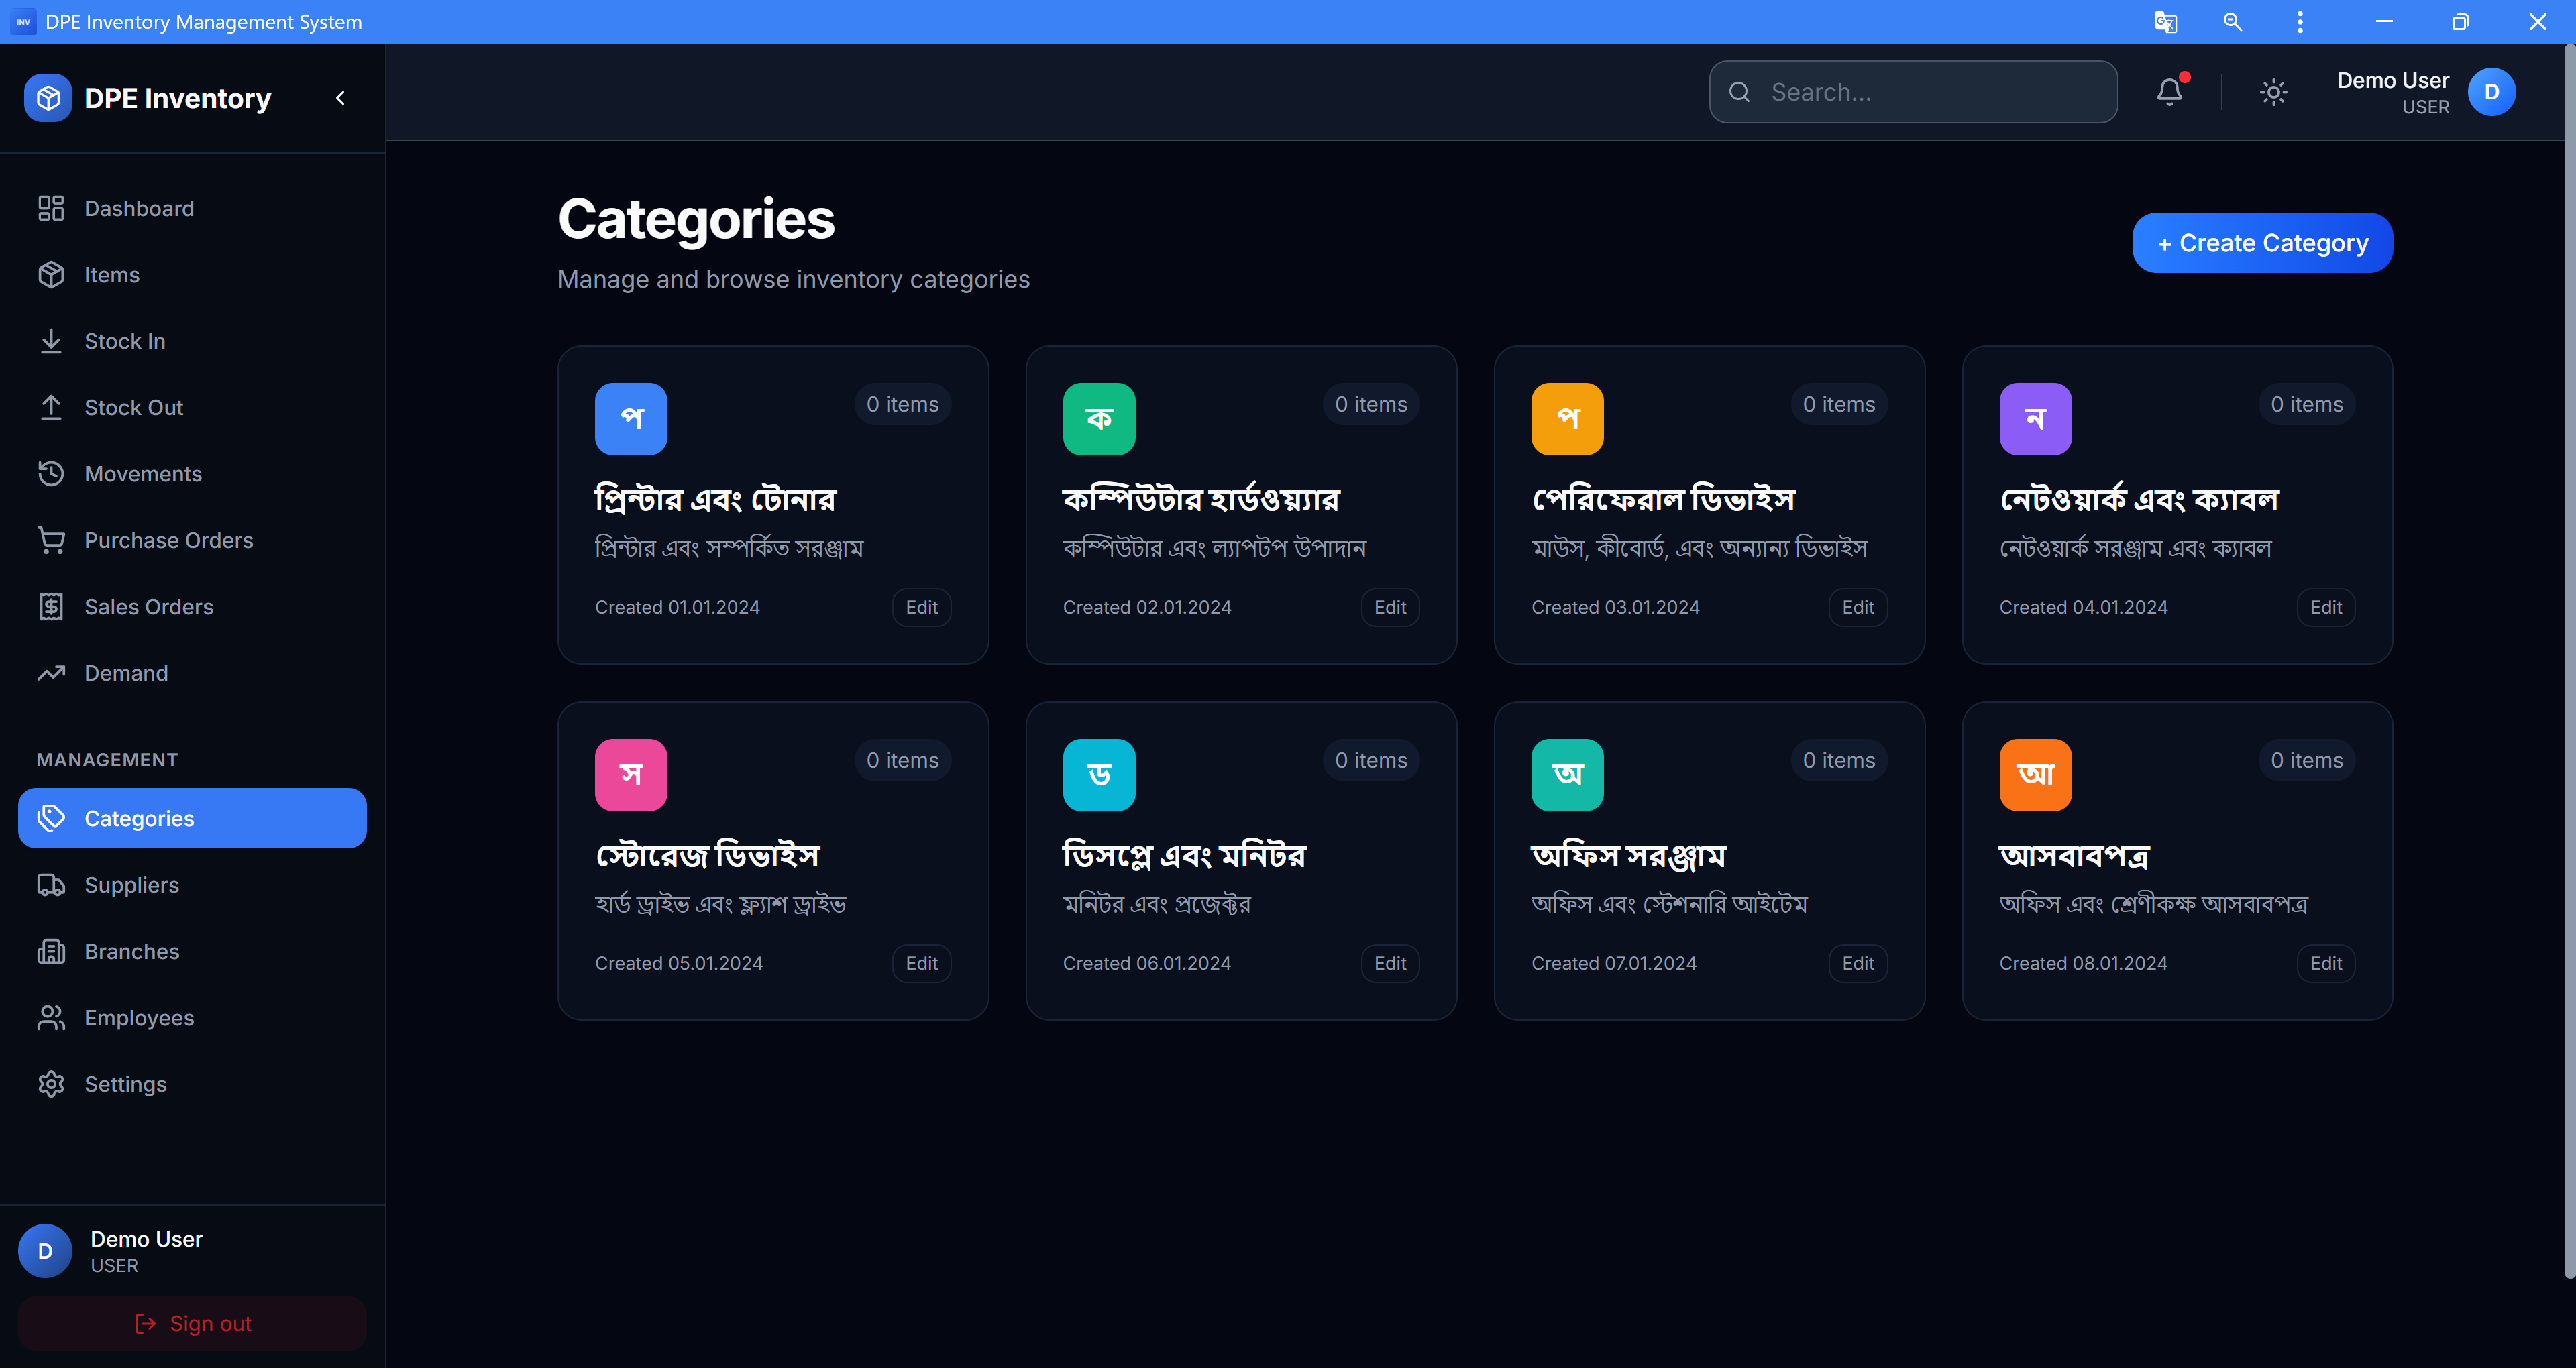
\includegraphics[width=3.6cm, height=2cm]{images/categories-dashboard.png}};
  \node[font=\tiny\bfseries, color=secondary] at (10.5,-4.2) {Category Management};
\end{tikzpicture}
\end{center}
\end{frame}

% ===================================================================
% SECTION: ROADMAP
% ===================================================================
\sectionpage{Implementation Roadmap}{From Planning to National Rollout}

% ===================================================================
% SLIDE 16 — TIMELINE
% ===================================================================
\begin{frame}{National Rollout Plan — 10 Months}
\vspace{0.2cm}
\begin{center}
\begin{tikzpicture}[scale=0.95]
  % Timeline base line
  \draw[line width=1.5pt, medgray!40] (0,0) -- (14,0);

  % Duration bars
  \draw[secondary, line width=3pt, opacity=0.3] (0.5,0) -- (2.5,0);
  \draw[accent, line width=3pt, opacity=0.3] (2.5,0) -- (5.5,0);
  \draw[warmgold, line width=3pt, opacity=0.3] (5.5,0) -- (8.5,0);
  \draw[primary, line width=3pt, opacity=0.3] (8.5,0) -- (11.5,0);
  \draw[accent, line width=3pt, opacity=0.3] (11.5,0) -- (14,0);

  % Phase 1
  \fill[secondary] (0.5,0) circle (6pt); \fill[white] (0.5,0) circle (3pt);
  \node[above=0.4cm, rounded corners=4pt, fill=secondary!8, draw=secondary!25,
        line width=0.3pt, inner sep=4pt, text width=2.2cm, font=\scriptsize] at (0.5,0) {%
    {\color{secondary}\faIcon{clipboard-list}~\textbf{Phase 1}}\\
    {\color{medgray}2 mo}\\Planning \& Requirements
  };

  % Phase 2
  \fill[accent] (3.5,0) circle (6pt); \fill[white] (3.5,0) circle (3pt);
  \node[above=0.4cm, rounded corners=4pt, fill=accent!8, draw=accent!25,
        line width=0.3pt, inner sep=4pt, text width=2.2cm, font=\scriptsize] at (3.5,0) {%
    {\color{accent}\faIcon{code}~\textbf{Phase 2}}\\
    {\color{medgray}3 mo}\\Development \& Build
  };

  % Phase 3
  \fill[warmgold] (7,0) circle (6pt); \fill[white] (7,0) circle (3pt);
  \node[above=0.4cm, rounded corners=4pt, fill=warmgold!8, draw=warmgold!25,
        line width=0.3pt, inner sep=4pt, text width=2.2cm, font=\scriptsize] at (7,0) {%
    {\color{warmgold}\faIcon{vial}~\textbf{Phase 3}}\\
    {\color{medgray}2 mo}\\Testing \& Pilot
  };

  % Phase 4
  \fill[primary] (10,0) circle (6pt); \fill[white] (10,0) circle (3pt);
  \node[above=0.4cm, rounded corners=4pt, fill=primary!8, draw=primary!25,
        line width=0.3pt, inner sep=4pt, text width=2.2cm, font=\scriptsize] at (10,0) {%
    {\color{primary}\faIcon{rocket}~\textbf{Phase 4}}\\
    {\color{medgray}3 mo}\\Training \& Rollout
  };

  % Phase 5
  \fill[accent] (13,0) circle (6pt); \fill[white] (13,0) circle (3pt);
  \node[above=0.4cm, rounded corners=4pt, fill=accent!8, draw=accent!25,
        line width=0.3pt, inner sep=4pt, text width=2.2cm, font=\scriptsize] at (13,0) {%
    {\color{accent}\faIcon{sync-alt}~\textbf{Phase 5}}\\
    {\color{medgray}Ongoing}\\Continuous Improvement
  };
\end{tikzpicture}
\end{center}

\vspace{0.4cm}
\begin{center}

\begin{tikzpicture}
  \node[rounded corners=5pt, fill=accent!10, inner sep=8pt] {%
    {\color{accent}\faIcon{flag-checkered}~\textbf{Deliverable: System deployed across 66,000+ schools with trained staff at every tier.}}
  };
\end{tikzpicture}
\end{center}
\end{frame}

% ===================================================================
% SLIDE 17 — KEY FEATURES SUMMARY
% ===================================================================
\begin{frame}{Key Features at a Glance}
\begin{columns}[T]
\column{0.48\textwidth}
\begin{tikzpicture}
  \node[rounded corners=6pt, fill=secondary!6, draw=secondary!20, line width=0.3pt,
        inner sep=8pt, text width=6cm] {%
    \textbf{\color{secondary}\faIcon{link}~Supply Chain Management}\\[6pt]
    \begin{minipage}{5.5cm}\small
    \iconbullet[secondary]{\faIcon{warehouse}}{Warehouse \& storage management}\\[3pt]
    \iconbullet[secondary]{\faIcon{shopping-cart}}{Automated procurement}\\[3pt]
    \iconbullet[secondary]{\faIcon{boxes}}{Real-time inventory tracking}\\[3pt]
    \iconbullet[secondary]{\faIcon{truck}}{Distribution monitoring}\\[3pt]
    \iconbullet[secondary]{\faIcon{chart-line}}{Demand forecasting}
    \end{minipage}
  };
\end{tikzpicture}

\vspace{0.3cm}
\begin{tikzpicture}
  \node[rounded corners=6pt, fill=warmgold!8, draw=warmgold!25, line width=0.3pt,
        inner sep=8pt, text width=6cm] {%
    \textbf{\color{warmgold}\faIcon{plug}~Integration \& Support}\\[6pt]
    \begin{minipage}{5.5cm}\small
    \iconbullet[warmgold]{\faIcon{exchange-alt}}{Seamless data flow with existing systems}\\[3pt]
    \iconbullet[warmgold]{\faIcon{language}}{Multi-language (Bangla/English)}\\[3pt]
    \iconbullet[warmgold]{\faIcon{chalkboard-teacher}}{User training programs}
    \end{minipage}
  };
\end{tikzpicture}

\column{0.48\textwidth}
\begin{tikzpicture}
  \node[rounded corners=6pt, fill=accent!6, draw=accent!20, line width=0.3pt,
        inner sep=8pt, text width=6cm] {%
    \textbf{\color{accent}\faIcon{gavel}~Governance \& Compliance}\\[6pt]
    \begin{minipage}{5.5cm}\small
    \iconbullet[accent]{\faIcon{history}}{Complete audit trails}\\[3pt]
    \iconbullet[accent]{\faIcon{user-lock}}{Role-based access control}\\[3pt]
    \iconbullet[accent]{\faIcon{shield-alt}}{Feature-based permissions (FBAC)}\\[3pt]
    \iconbullet[accent]{\faIcon{hand-holding-usd}}{Financial accountability}\\[3pt]
    \iconbullet[accent]{\faIcon{ban}}{Misuse prevention}
    \end{minipage}
  };
\end{tikzpicture}

\vspace{0.3cm}

\begin{tikzpicture}
  \node[rounded corners=6pt, fill=primary!5, draw=primary!15, line width=0.3pt,
        inner sep=8pt, text width=6cm] {%
    \textbf{\color{primary}\faIcon{chart-bar}~Analytics \& Reporting}\\[6pt]
    \begin{minipage}{5.5cm}\small
    \iconbullet[primary]{\faIcon{tachometer-alt}}{Real-time dashboards}\\[3pt]
    \iconbullet[primary]{\faIcon{file-pdf}}{One-click report generation}\\[3pt]
    \iconbullet[primary]{\faIcon{brain}}{Budget planning insights}
    \end{minipage}
  };
\end{tikzpicture}
\end{columns}
\end{frame}

% ===================================================================
% SECTION: WHY FINKOPS
% ===================================================================
\sectionpage{Why FinkOps}{German Engineering Meets National Impact}

% ===================================================================
% SLIDE 18 — WHY CHOOSE US
% ===================================================================
\begin{frame}{Why Choose FinkOps (Germany)}
\begin{columns}[T]
\column{0.48\textwidth}

\begin{tikzpicture}
  \node[rounded corners=6pt, fill=secondary!6, draw=secondary!20, line width=0.3pt,
        inner sep=8pt, text width=6cm] {%
    \textbf{\color{secondary}\faIcon{microchip}~Technical Strength}\\[6pt]
    \begin{minipage}{5.5cm}\small
    \iconbullet[secondary]{\faIcon{cog}}{German precision \& reliability}\\[3pt]
    \iconbullet[secondary]{\faIcon{shield-alt}}{Security-first architecture}\\[3pt]
    \iconbullet[secondary]{\faIcon{certificate}}{ISO27001-aligned workflows}\\[3pt]
    \iconbullet[secondary]{\faIcon{expand-arrows-alt}}{Massive-scale system expertise}
    \end{minipage}
  };
\end{tikzpicture}

\vspace{0.3cm}
\begin{tikzpicture}
  \node[rounded corners=6pt, fill=accent!6, draw=accent!20, line width=0.3pt,
        inner sep=8pt, text width=6cm] {%
    \textbf{\color{accent}\faIcon{bullseye}~Tailored for DPE}\\[6pt]
    \begin{minipage}{5.5cm}\small
    \iconbullet[accent]{\faIcon{list-alt}}{Exact DPE item catalog alignment}\\[3pt]
    \iconbullet[accent]{\faIcon{language}}{Bangla/English UI}\\[3pt]
    \iconbullet[accent]{\faIcon{school}}{School-level workflows}\\[3pt]
    \iconbullet[accent]{\faIcon{rocket}}{Fast rollout readiness}
    \end{minipage}
  };
\end{tikzpicture}

\column{0.48\textwidth}
\begin{tikzpicture}
  \node[rounded corners=6pt, fill=warmgold!8, draw=warmgold!25, line width=0.3pt,
        inner sep=8pt, text width=6cm] {%
    \textbf{\color{warmgold}\faIcon{trophy}~Track Record}\\[6pt]
    \begin{minipage}{5.5cm}\small
    \iconbullet[warmgold]{\faIcon{clock}}{15+ years supply chain automation}\\[3pt]
    \iconbullet[warmgold]{\faIcon{building}}{Fortune 500 enterprise platforms}\\[3pt]
    \iconbullet[warmgold]{\faIcon{landmark}}{Government \& public sector proven}\\[3pt]
    \iconbullet[warmgold]{\faIcon{flag}}{German engineering standards}
    \end{minipage}
  };
\end{tikzpicture}

\vspace{0.3cm}
\begin{tikzpicture}
  \node[rounded corners=6pt, fill=primary!5, draw=primary!15, line width=0.3pt,
        inner sep=8pt, text width=6cm] {%
    \textbf{\color{primary}\faIcon{hammer}~What We've Built}\\[6pt]
    \begin{minipage}{5.5cm}\small
    \iconbullet[primary]{\faIcon{warehouse}}{Real-time WMS systems}\\[3pt]
    \iconbullet[primary]{\faIcon{project-diagram}}{Multi-tier distribution networks}\\[3pt]
    \iconbullet[primary]{\faIcon{clipboard-check}}{Compliance audit systems}\\[3pt]
    \iconbullet[primary]{\faIcon{cloud}}{Cloud-native architectures}
    \end{minipage}
  };
\end{tikzpicture}
\end{columns}
\end{frame}

% ===================================================================
% SLIDE 19 — WORK EXPERIENCE
% ===================================================================
\begin{frame}{FinkOps Enterprise Experience}
\vspace{0.1cm}
\begin{center}
\begin{tikzpicture}[
  expcard/.style={rounded corners=5pt, fill=#1!7, draw=#1!20, line width=0.3pt,
    minimum width=4.6cm, minimum height=1.5cm, inner sep=5pt}
]
  % Row 1
  \node[expcard=secondary] at (0,0) {%
    \begin{minipage}{4.2cm}
      {\color{secondary}\faIcon{university}~\textbf{\small Banking Systems}}\\
      {\scriptsize Core banking, payment processing, account management}
    \end{minipage}};
  \node[expcard=accent] at (5.2,0) {%
    \begin{minipage}{4.2cm}
      {\color{accent}\faIcon{boxes}~\textbf{\small Inventory Management}}\\
      {\scriptsize Real-time tracking, multi-warehouse, auto-reordering}
    \end{minipage}};
  \node[expcard=warmgold] at (10.4,0) {%
    \begin{minipage}{4.2cm}
      {\color{warmgold}\faIcon{users-cog}~\textbf{\small HR Management}}\\
      {\scriptsize Employee databases, payroll, performance tracking}
    \end{minipage}};
  % Row 2
  \node[expcard=primary] at (0,-2.1) {%
    \begin{minipage}{4.2cm}
      {\color{primary}\faIcon{shopping-bag}~\textbf{\small E-Commerce}}\\
      {\scriptsize Product catalogs, order management, customer portals}
    \end{minipage}};
  \node[expcard=danger] at (5.2,-2.1) {%
    \begin{minipage}{4.2cm}
      {\color{danger}\faIcon{truck}~\textbf{\small Delivery Systems}}\\
      {\scriptsize Route optimization, real-time tracking, fleet management}
    \end{minipage}};
  \node[expcard=secondary] at (10.4,-2.1) {%
    \begin{minipage}{4.2cm}
      {\color{secondary}\faIcon{project-diagram}~\textbf{\small Supply Chain}}\\
      {\scriptsize Multi-tier distribution, forecasting, compliance}
    \end{minipage}};
\end{tikzpicture}
\end{center}

\vspace{0.2cm}
\begin{center}

\begin{tikzpicture}
  \node[rounded corners=4pt, fill=accent!10, inner sep=6pt] {%
    {\color{accent}\faIcon{check-double}~\textbf{Proven expertise across industries. Purpose-built for DPE.}}
  };
\end{tikzpicture}
\end{center}
\end{frame}

% ===================================================================
% SLIDE 20 — ABOUT FINKOPS
% ===================================================================
\begin{frame}{About FinkOps UG (Germany)}
\begin{columns}[T]
\column{0.55\textwidth}
\vspace{0.2cm}
\textbf{\color{primary}Who We Are:}\\[4pt]
{\small FinkOps UG (haftungsbeschr\"ankt) is a German software engineering company specializing in enterprise-scale supply chain and inventory management solutions.}

\vspace{0.4cm}
\textbf{\color{primary}Why Government Trusts Us:}
\begin{itemize}\small
  \item[\color{accent}\faIcon{check}] Secure, auditable systems for public institutions
  \item[\color{accent}\faIcon{check}] Scalable solutions for national-level deployments
  \item[\color{accent}\faIcon{check}] Data protection \& compliance expertise
  \item[\color{accent}\faIcon{check}] Long-term partnership approach
  \item[\color{accent}\faIcon{check}] ISO27001 certified security implementations
  \item[\color{accent}\faIcon{check}] Transparent, reliable operations
\end{itemize}

\column{0.42\textwidth}
\vspace{0.2cm}
\begin{center}

\begin{tikzpicture}
  \node[rounded corners=8pt, fill=primary!5, draw=primary!15, line width=0.3pt,
        inner sep=12pt, text width=5cm] {%
    \centering
    {\color{primary}\fontsize{36}{40}\selectfont\faIcon{globe-europe}}\\[10pt]
    {\color{primary}\large\bfseries German Precision}\\[4pt]
    {\color{accent}\normalsize Meets Global Impact}\\[12pt]
    {\color{medgray}\small Ready to transform\\Bangladesh's primary\\education system.}
  };
\end{tikzpicture}
\end{center}
\end{columns}
\end{frame}

% ===================================================================
% SECTION: Q&A
% ===================================================================
\sectionpage{Questions \& Discussion}{We're Here to Answer Your Questions}

% ===================================================================
% SLIDE 21 — COMMON QUESTIONS
% ===================================================================
\begin{frame}{Common Questions}
\begin{tikzpicture}[
  qabox/.style={rounded corners=5pt, fill=softgray, inner sep=7pt, text width=\textwidth-1cm}
]
  \node[qabox] at (0,0) {%
    {\color{secondary}\faIcon{question-circle}~\textbf{How long will implementation take?}}\\[3pt]
    {\small\color{accent}\faIcon{arrow-right}}~{\small 10 months total: Planning $\rightarrow$ Development $\rightarrow$ Testing $\rightarrow$ Rollout $\rightarrow$ Support}
  };
  \node[qabox] at (0,-1.7) {%
    {\color{secondary}\faIcon{question-circle}~\textbf{Will the system work with poor internet connectivity?}}\\[3pt]
    {\small\color{accent}\faIcon{arrow-right}}~{\small Yes. PWA technology enables offline-first operation with automatic sync when connectivity returns.}
  };
  \node[qabox] at (0,-3.4) {%
    {\color{secondary}\faIcon{question-circle}~\textbf{How is data security ensured?}}\\[3pt]
    {\small\color{accent}\faIcon{arrow-right}}~{\small RBAC + FBAC, 2FA, encryption at rest/transit, immutable audit logs, ISO27001-aligned architecture.}
  };
  \node[qabox] at (0,-5.1) {%
    {\color{secondary}\faIcon{question-circle}~\textbf{Can the system scale to 66,000+ schools?}}\\[3pt]
    {\small\color{accent}\faIcon{arrow-right}}~{\small Yes. Built on microservices, Kubernetes, and cloud-native architecture designed for national scale.}
  };
\end{tikzpicture}
\end{frame}

% ===================================================================
% SLIDE 22 — CONTACT
% ===================================================================
\begin{frame}{Contact Us}
\begin{columns}[T]
\column{0.48\textwidth}
\begin{tikzpicture}
  \node[rounded corners=8pt, fill=secondary!6, draw=secondary!20, line width=0.3pt,
        inner sep=12pt, text width=5.5cm] {%
    {\color{secondary}\Large\faIcon{building}~\textbf{FinkOps Germany}}\\[8pt]
    {\small\textbf{FinkOps UG (haftungsbeschr\"ankt)}}\\[6pt]
    {\small\color{medgray}Goethestra\ss e 127\\63477 Maintal, Germany}\\[8pt]
    {\small\faIcon{envelope}~\href{mailto:contact@finkops.com}{\color{secondary}contact@finkops.com}}\\[3pt]
    {\small\faIcon{phone}~+49 15560 354545}\\[3pt]
    {\small\faIcon{globe}~\href{https://finkops.com/}{\color{secondary}finkops.com}}
  };
\end{tikzpicture}

\column{0.48\textwidth}

\begin{tikzpicture}
  \node[rounded corners=8pt, fill=accent!6, draw=accent!20, line width=0.3pt,
        inner sep=12pt, text width=5.5cm] {%
    {\color{accent}\Large\faIcon{handshake}~\textbf{Bangladesh Partner}}\\[8pt]
    {\small\textbf{SyntaxFlow Software}}\\[6pt]
    {\small\color{medgray}Bangladesh Implementation Partner\\Bangladesh Office}\\[8pt]
    {\small\faIcon{envelope}~\href{mailto:contact@syntaxflowsoftware.com}{\color{accent}contact@syntaxflowsoftware.com}}\\[3pt]
    {\small\faIcon{phone}~+880 1744 633922}\\[3pt]
    {\small\faIcon{globe}~\href{https://syntaxflowsoftware.com/}{\color{accent}syntaxflowsoftware.com}}
  };
\end{tikzpicture}
\end{columns}

\vspace{0.5cm}
\begin{center}

\begin{tikzpicture}
  \node[rounded corners=5pt, fill=warmgold!10, inner sep=8pt] {%
    {\color{warmgold}\faIcon{handshake}~\textbf{Partnership for Success — German Engineering \& Local Expertise}}
  };
\end{tikzpicture}
\end{center}
\end{frame}

% ===================================================================
% SLIDE 23 — THE VISION (Closing)
% ===================================================================
\begin{frame}[plain]

\begin{tikzpicture}[remember picture, overlay]
  \fill[left color=gradstart, right color=gradend] (current page.south west) rectangle (current page.north east);
  \fill[white, opacity=0.03] ([xshift=-4cm, yshift=3cm]current page.south east) circle (8cm);
  \fill[accent, opacity=0.06] ([xshift=5cm, yshift=-2cm]current page.north west) circle (5cm);

  \node[anchor=center, text=white] at ([yshift=1cm]current page.center) {%
    \begin{minipage}{0.75\textwidth}\centering
      {\fontsize{11}{14}\selectfont\color{accentlight}THE VISION}\\[14pt]
      {\fontsize{20}{24}\selectfont\bfseries Bangladesh has already scaled\\education to millions.}\\[14pt]
      {\fontsize{20}{24}\selectfont\bfseries Now it will scale transparency,\\efficiency, and governance.}\\[18pt]
      {\color{accent}\rule{6cm}{2pt}}\\[14pt]
      {\Large\color{warmgold}\textbf{FinkOps is your partner for that transformation.}}
    \end{minipage}
  };
\end{tikzpicture}
\end{frame}

% ===================================================================
% SLIDE 24 — THANK YOU
% ===================================================================
\begin{frame}[plain]
\begin{tikzpicture}[remember picture, overlay]
  \fill[primary] (current page.south west) rectangle (current page.north east);
  \fill[secondary, opacity=0.12] ([xshift=6cm]current page.south west) circle (7cm);
  \fill[accent, opacity=0.08] ([xshift=-4cm, yshift=-2cm]current page.north east) circle (4cm);

  % Logo
  \node[anchor=north] at ([yshift=-1.5cm]current page.north) {%
    
\includegraphics[height=1.2cm]{images/government-bangladesh-logo.png}
  };

  \node[anchor=center, text=white] at ([yshift=-0.3cm]current page.center) {%
    \begin{minipage}{0.7\textwidth}\centering
      {\fontsize{36}{40}\selectfont\bfseries Thank You}\\[16pt]
      {\large\color{softgray}Transforming Bangladesh's Primary Education\\Supply Chain System}\\[20pt]
      {\color{accent}\rule{5cm}{1.5pt}}\\[14pt]
      {\normalsize\color{accentlight}\faIcon{building}~FinkOps UG (haftungsbeschr\"ankt)}\\[4pt]
      {\small\color{medgray}German Engineering for National-Scale Impact}\\[12pt]
      {\small\color{warmgold}\faIcon{envelope}~contact@finkops.com \hspace{1cm} \faIcon{globe}~finkops.com}
    \end{minipage}
  };
\end{tikzpicture}
\end{frame}

\end{document}
